% --------------------------------------------------------------------------- %
% --------------------------------------------------------------------------- %
\chapter{Analysis Selections}
\label{ch:evtsel}
% --------------------------------------------------------------------------- %
% --------------------------------------------------------------------------- %

\section{Triggers and Datasets}
The signal triggers used in this analysis were designed to be maximally efficient for events where a Z boson decays to two leptons.
In order to pass the trigger, at least two leptons with a loose ID and isolation requirement are needed.
Then lepton \pt\ thresholds of the triggers are low enough such that the triggers are fully efficient after making an offline \pt\ cut at 20 \gev\ for both the leading and sub-leading lepton in the event.
In addition to the signal triggers, two other sets of triggers are used in order to collect data in control regions used for data-driven background predictions in the signal region,
and a last set of triggers is used to collect data used to measure the efficiency of the dilepton triggers.
The efficiencies of the ee, e$\mu$ and $\mu\mu$ triggers with respect to the offline selection with two leptons with \pt\ $>$ 20 GeV have been measured as 0.95, 0.94 and 0.93 respectively.
The way this measurement was made is described in section~\ref{sec:bkg_fs}.
All triggers used to collect data for this analysis are listed in table~\ref{table:triggers}.

\begin{itemize}
\item Datasets
  \begin{itemize}
  \item \verb=DoubleEG=
  \item \verb=DoubleMuon=
  \item \verb=MuonEG=
  \item \verb=SinglePhoton=
  \end{itemize}
\item Datasets
  \begin{itemize}
  \item \verb=Run2015C-05Oct2015-v1=
  \item \verb=Run2015D-05Oct2015-v1=
  \item \verb=Run2015D-PromptReco-v4=
  \end{itemize}
\end{itemize}

\begin{table}[htb]
  \begin{center}
    \caption{
      \label{table:triggers}
      List of all triggers used in this analysis.
    }
    \begin{tabular}{l}
      \hline
      \hline
      {\bf Signal triggers} \\
      \hline
      \verb=HLT_Mu17_TrkIsoVVL_Mu8_TrkIsoVVL_DZ_v*=             \\
      \verb=HLT_Mu17_TrkIsoVVL_TkMu8_TrkIsoVVL_DZ_v*=           \\
      \verb=HLT_Mu27_TkMu8_v*=                                  \\
      \verb=HLT_Ele17_Ele12_CaloIdL_TrackIdL_IsoVL_DZ_v*=       \\
      \verb=HLT_DoubleEle33_CaloIdL_GsfTrkIdVL_MW_v*=           \\
      \hline
      {\bf e$\mu$ triggers} \\
      \hline
      \verb=HLT_Mu17_TrkIsoVVL_Ele12_CaloIdL_TrackIdL_IsoVL_v*= \\
      \verb=HLT_Mu8_TrkIsoVVL_Ele17_CaloIdL_TrackIdL_IsoVL_v*=  \\
      \verb=HLT_Mu30_Ele30_CaloIdL_GsfTrkIdVL_v*=               \\
      \hline
      {\bf single-$\gamma$ triggers} \\
      \hline
      \verb=HLT_Photon22_R9Id90_HE10_IsoM_v*=  \\ 
      \verb=HLT_Photon30_R9Id90_HE10_IsoM_v*=  \\
      \verb=HLT_Photon36_R9Id90_HE10_IsoM_v*=  \\
      \verb=HLT_Photon50_R9Id90_HE10_IsoM_v*=  \\
      \verb=HLT_Photon75_R9Id90_HE10_IsoM_v*=  \\
      \verb=HLT_Photon90_R9Id90_HE10_IsoM_v*=  \\
      \verb=HLT_Photon120_R9Id90_HE10_IsoM_v*= \\
      \verb=HLT_Photon165_R9Id90_HE10_IsoM_v*= \\
      \verb=HLT_Photon165_HE10_v*=             \\
      \hline
      {\bf \HT\ triggers} \\
      \hline
      \verb=HLT_PFHT200_v*= \\
      \verb=HLT_PFHT250_v*= \\
      \verb=HLT_PFHT300_v*= \\
      \verb=HLT_PFHT350_v*= \\
      \verb=HLT_PFHT400_v*= \\
      \verb=HLT_PFHT475_v*= \\
      \verb=HLT_PFHT600_v*= \\
      \verb=HLT_PFHT650_v*= \\
      \verb=HLT_PFHT800_v*= \\
      \verb=HLT_PFHT900_v*= \\
      \hline
      \hline

    \end{tabular}
  \end{center}
\end{table}

\clearpage

\section{Simulations from Monte-Carlo}
The CMS detector is simulated using the Geant4 toolbox~\cite{Geant}, and various physics processes are simulated.
The simulation is composed of the following steps
\begin{itemize}
\item Modeling the Interaction Region
\item Modeling the particles passage through the hierarchy of volumes that compose CMS detector and of the accompanying physics processes
\item Modeling the effects of multiple interactions per beam crossing and/or the effect of events overlay (PileUp simulation)
\item Modeling the detector's electronics response (digitization)
\end{itemize}

The actual simulation of the physics process is done using a variety of different software where the various packages used perform differently at simulating certain physics effects.
In this analysis, \ttbar\ events are simulated using powheg~\cite{powheg} and DY processes are simulated using MadGraph~\cite{aMCatNLO}.
The matrix element calculations performed with these generators are then interfaced with pythia 8~\cite{Pythia} for the simulation of parton showering and hadronization.

After selecting events with two leptons, data is compared to MC and good agreement can be seen in the plots shown in section~\ref{ssec:datavsmc}.
Cross sections and k-factors are applied to MC backgrounds to normalize them to the calculated luminosity of the signal triggers used to take data in 2015, which is 2.3 $\mathrm{fb^{-1}}$.
Cross section values are calculated using the FEWZ software package~\cite{Li:2012wna},
and factors are derived by comparing data to MC in control regions in order to correct the MC for beyond leading-order effects. %%https://twiki.cern.ch/twiki/bin/viewauth/CMS/SummaryTable1G25ns
The events from MC are required to pass the same triggers as in data where the triggers are simulated in the MC,
and the MC is then reweighted to accurately represent the number of pileup events in data.

\begin{sidewaystable}[htb]                                                                                                                                                              
\begin{center}                                                                                                                                                
%% \scriptsize
\caption{\label{tab:mcsamples} List of MC samples.}
\begin{tabular}{l|l|l}  
\hline
\hline
Process     & Dataset Name                                                                & Cross Section [pb] \\
\hline
\zjets      & \verb=/DYJetsToLL_M-10to50_TuneCUETP8M1_13TeV-amcatnloFXFX-pythia8/*=       & 18610        \\
            & \verb=/DYJetsToLL_M-50_TuneCUETP8M1_13TeV-amcatnloFXFX-pythia8/*=           & 6104         \\
\hline
\ttbar      & \verb=/TTTo2L2Nu_13TeV-powheg/*=                                            & 87.31483776  \\
\hline
ZZ          & \verb=/ZZTo4L_13TeV_powheg_pythia8*=                                        & 1.256        \\
            & \verb=/ZZTo2L2Q_13TeV_amcatnloFXFX_madspin_pythia8/*=                       & 3.38         \\
            & \verb=/ZZTo2L2Nu_13TeV_powheg_pythia8/*=                                    &              \\
\hline
WZ          & \verb=/WZTo2L2Q_13TeV_amcatnloFXFX_madspin_pythia8/*=                       & 5.52         \\
            & \verb=/WZTo3LNu_TuneCUETP8M1_13TeV-powheg-pythia8/*=                        & 4.42965      \\
\hline
WW          & \verb=/WWTo2L2Nu_13TeV-powheg/*/=                                           & 118.7        \\
\hline
single top  & \verb=/ST_tW_top_5f_inclusiveDecays_13TeV-powheg-pythia8/*=                 & 38.09        \\
            & \verb=/ST_tW_antitop_5f_inclusiveDecays_13TeV-powheg-pythia8/*=             & 38.09        \\
\hline
${\ttbar}$V & \verb=/TTWJetsToLNu_TuneCUETP8M1_13TeV-amcatnloFXFX-madspin-pythia8/*=      & 0.2043       \\
            & \verb=/TTWJetsToQQ_TuneCUETP8M1_13TeV-amcatnloFXFX-madspin-pythia8/*=       & 0.40620      \\
            & \verb=/TTGJets_TuneCUETP8M1_13TeV-amcatnloFXFX-madspin-pythia8/*=           & 3.697        \\
            & \verb=/TTZToQQ_TuneCUETP8M1_13TeV-amcatnlo-pythia8/*=                       & 0.5297       \\
            & \verb=/TTZToLLNuNu_M-10_TuneCUETP8M1_13TeV-amcatnlo-pythia8/*=              & 0.2529       \\
            & \verb=/ttHToNonbb_M125_13TeV_powheg_pythia8/*=                              & 0.5085       \\
\hline
VVV         & \verb=/ZZZ_TuneCUETP8M1_13TeV-amcatnlo-pythia8/*=                           & 0.01398      \\
            & \verb=/WWZ_TuneCUETP8M1_13TeV-amcatnlo-pythia8/*=                           & 0.1651       \\
            & \verb=/WZZ_TuneCUETP8M1_13TeV-amcatnlo-pythia8/*=                           & 0.05565      \\
\hline
            & \verb=*RunIISpring15MiniAODv2-74X_mcRun2_asymptotic_v2-v*/MINIAODSIM=       &              \\
\hline
Signal      & \verb=SMS-T5ZZ_mGluino-*_mLSP-*_TuneCUETP8M1_13TeV-madgraphMLM-pythia8=     & See~\cite{gluinoxsec13tev} \\
\hline
\hline
\end{tabular}
\end{center}
\end{sidewaystable}

\clearpage

\subsection{Data vs. MC Comparison}
\label{ssec:datavsmc}
data is compared to MC simulation for many kinematic variables relevant to the search.

\begin{figure}[!ht]
  \begin{center}
    \begin{tabular}{cc}
      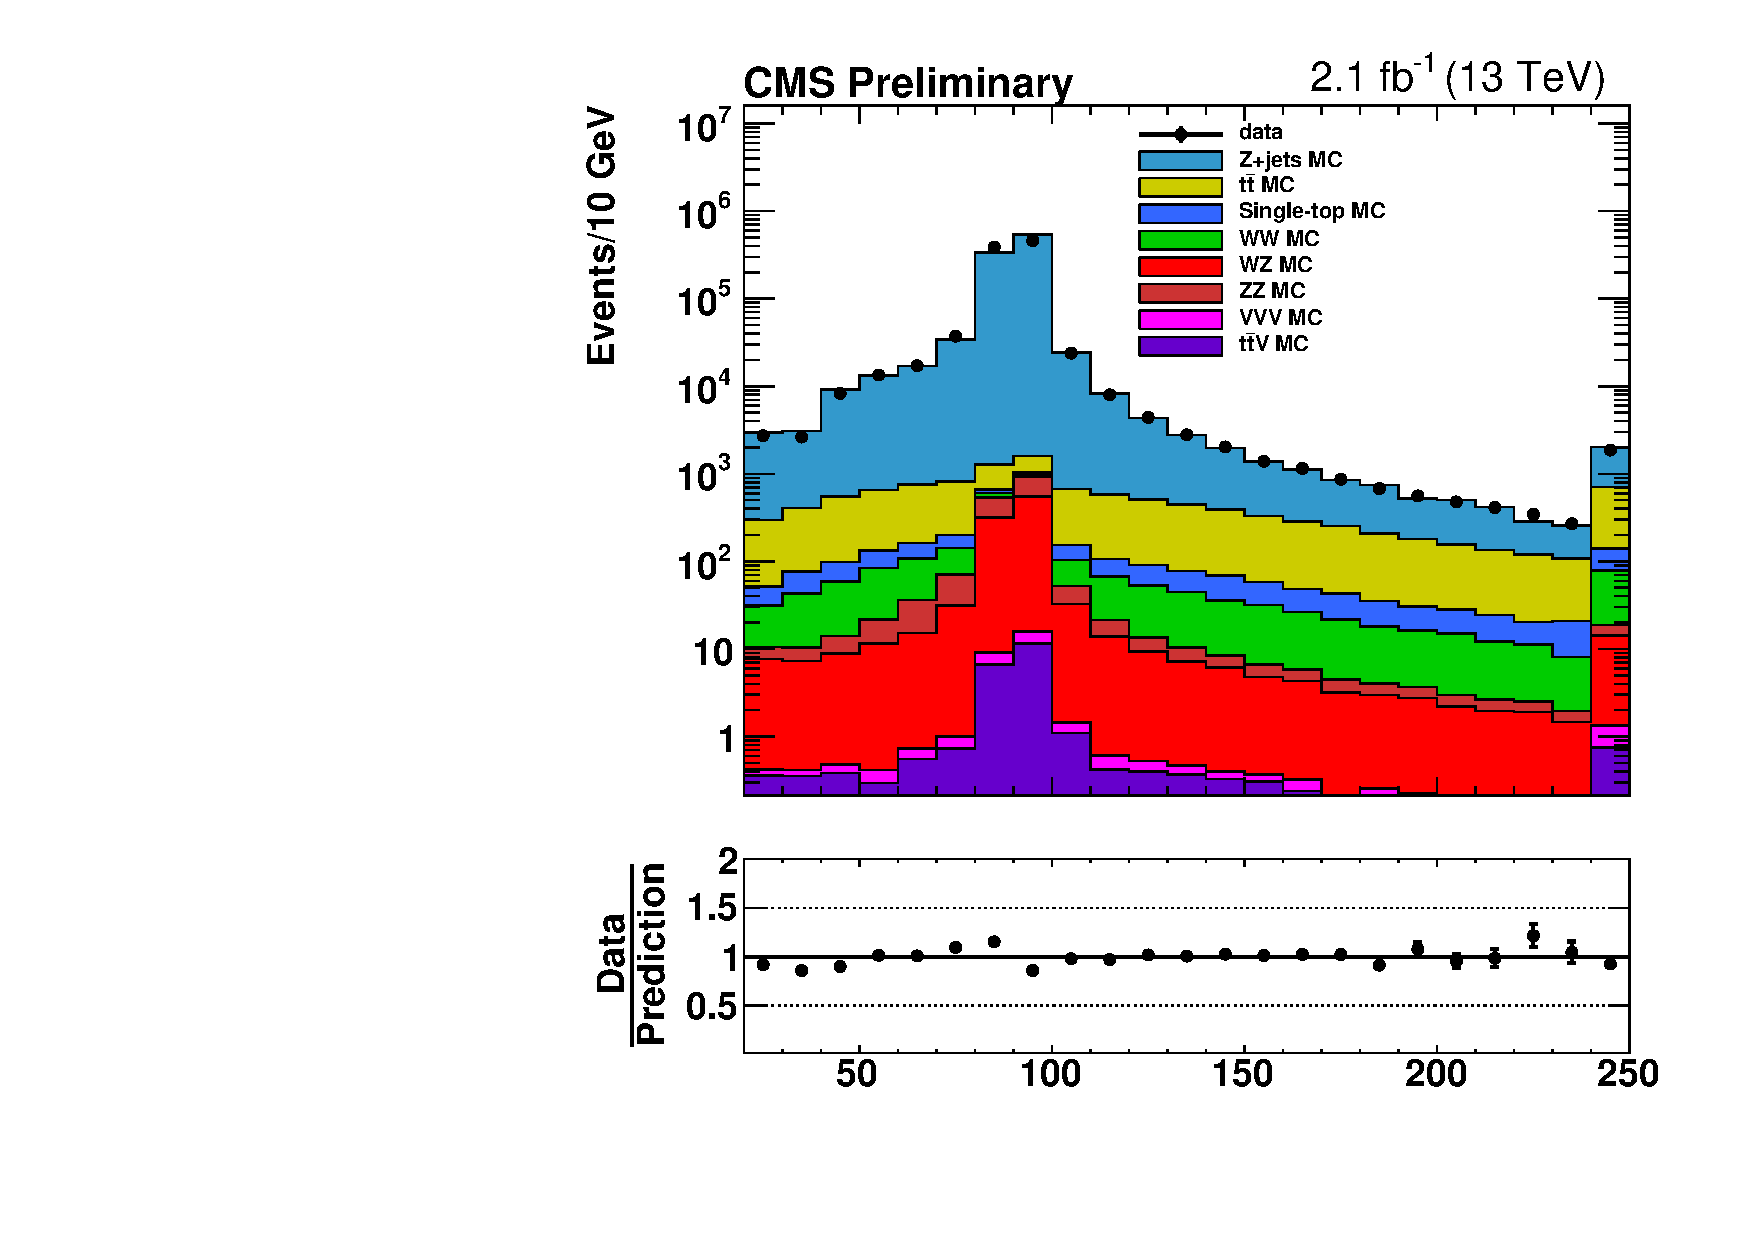
\includegraphics[width=0.4\linewidth]{evtsel/figs/h_mll_ee_signalregion_inclusive_passtrig.pdf} &
      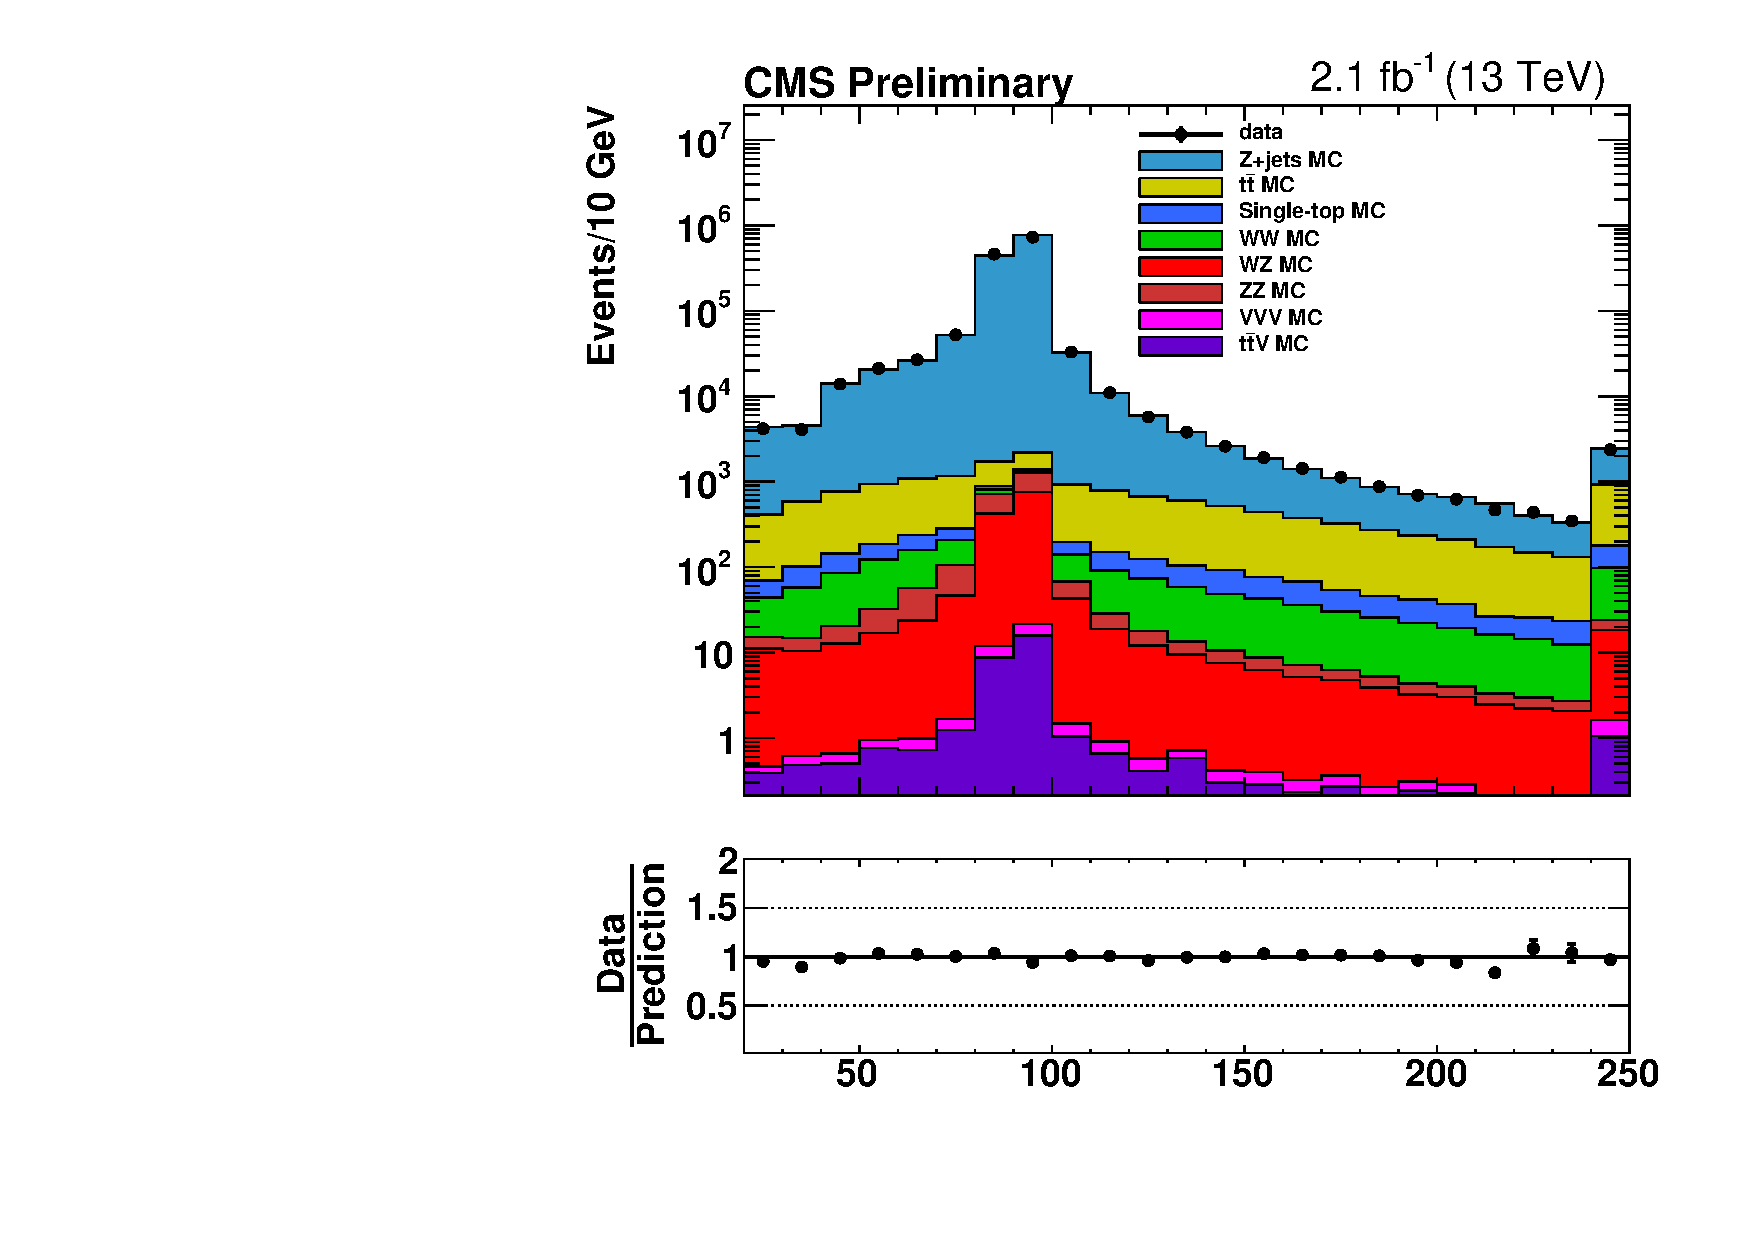
\includegraphics[width=0.4\linewidth]{evtsel/figs/h_mll_mm_signalregion_inclusive_passtrig.pdf} \\
    \end{tabular}
    \caption{
      \label{fig:datavsmc_mll_eemm}
      data vs. MC comparison showing \mll\ with ee events on the left and $\mu\mu$~events on the right.
    }
  \end{center}
\end{figure}

\begin{figure}[!ht]
  \begin{center}
    \begin{tabular}{cc}
      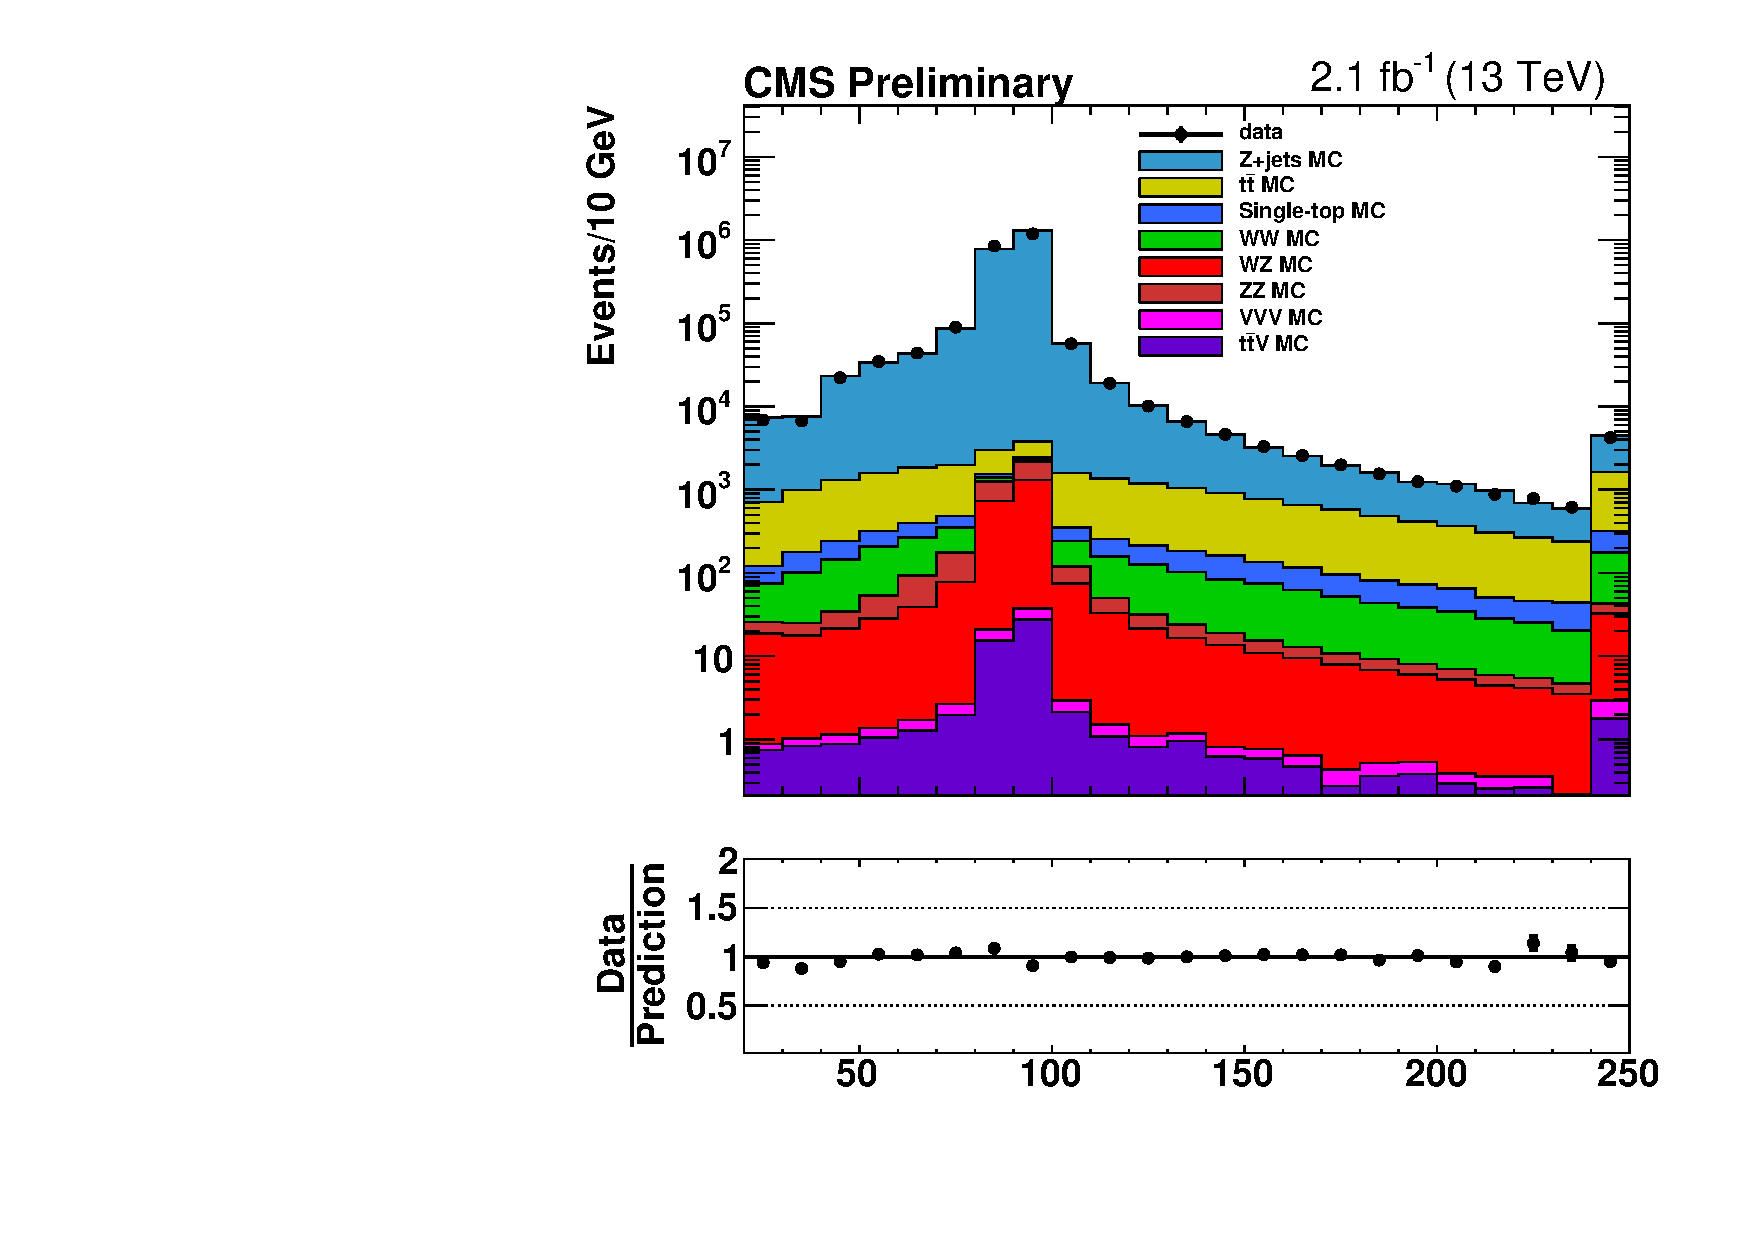
\includegraphics[width=0.4\linewidth]{evtsel/figs/h_mll_ll_signalregion_inclusive_passtrig.pdf} &
      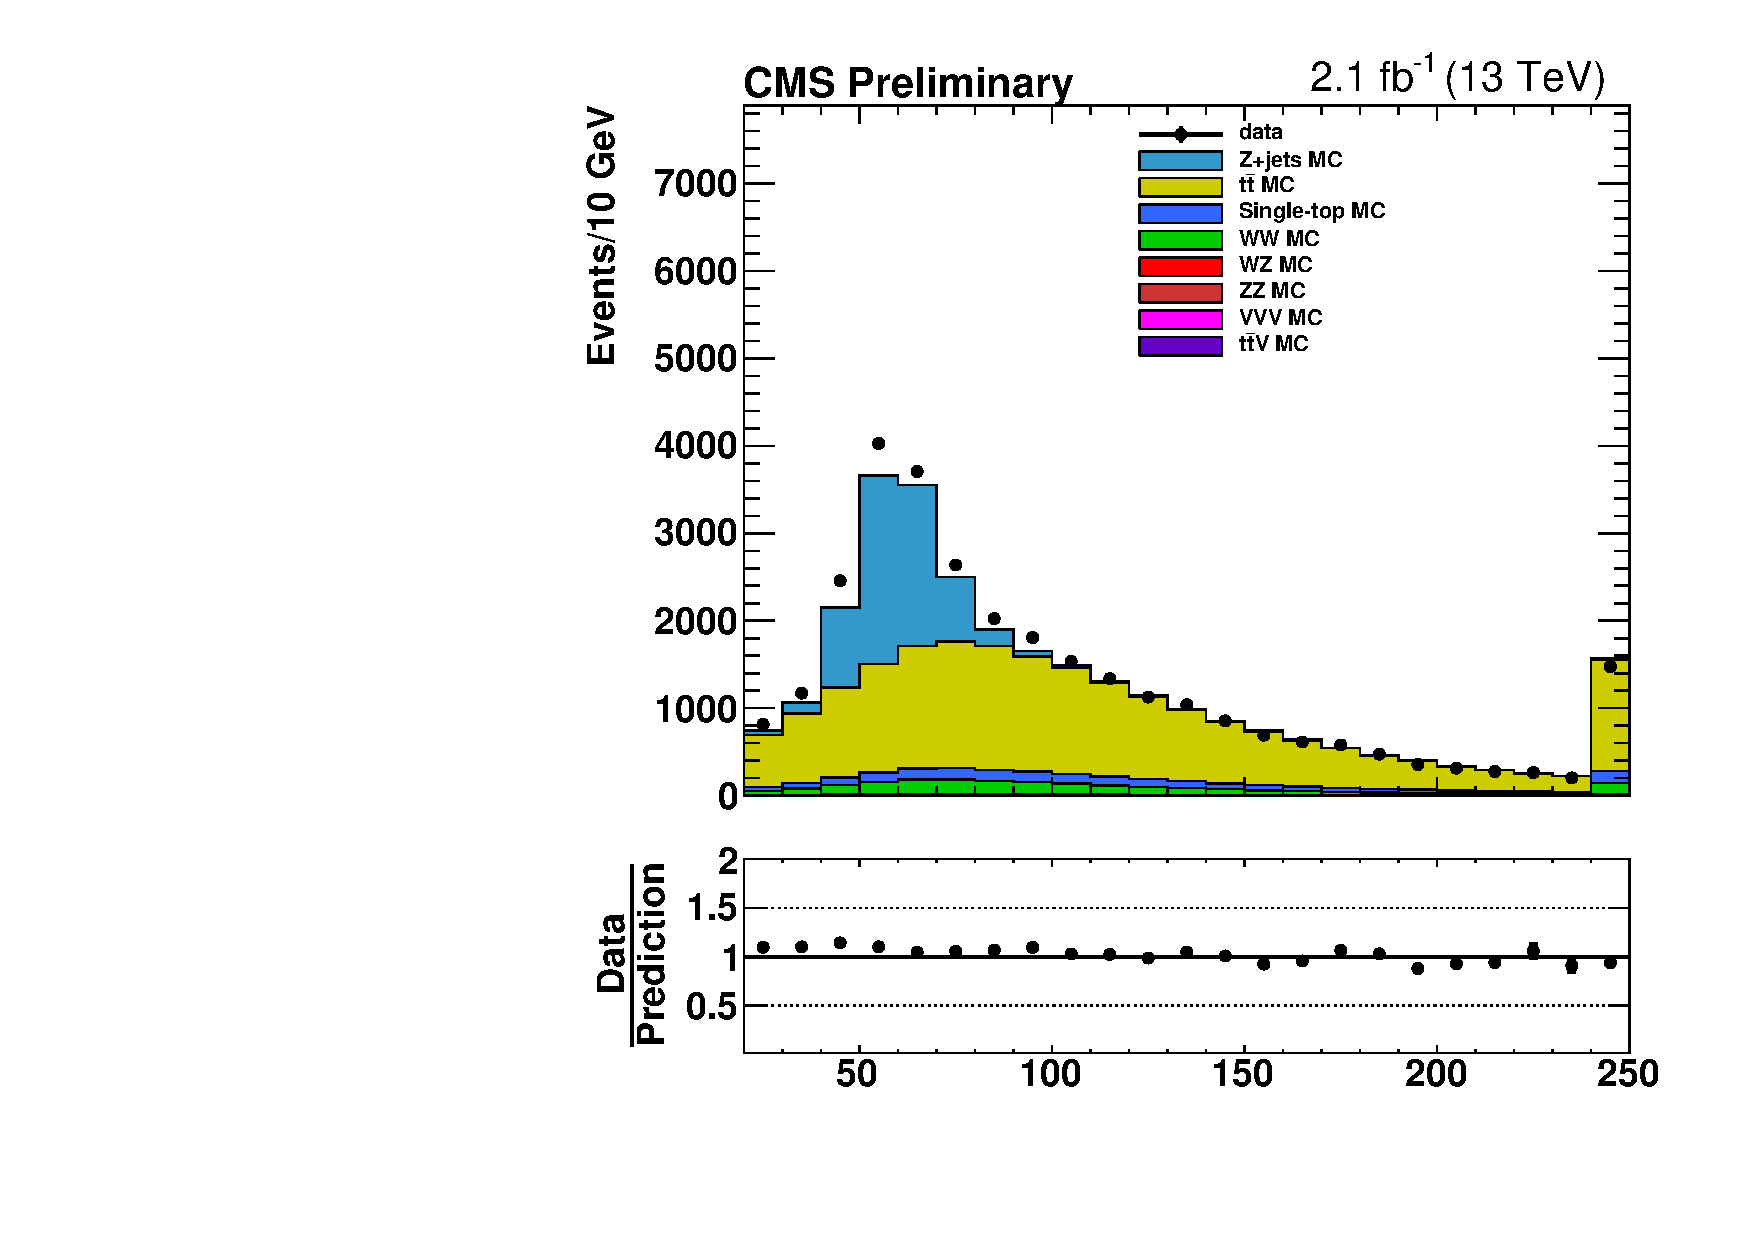
\includegraphics[width=0.4\linewidth]{evtsel/figs/h_mll_em_signalregion_inclusive_passtrig.pdf} \\
    \end{tabular}
    \caption{
      \label{fig:datavsmc_mll_emll}
      data vs. MC comparison showing \mll\ with ee+$\mu\mu$~events on the left and e$\mu$~events on the right.
    }
  \end{center}
\end{figure}

\begin{figure}[!ht]
  \begin{center}
    \begin{tabular}{cc}
      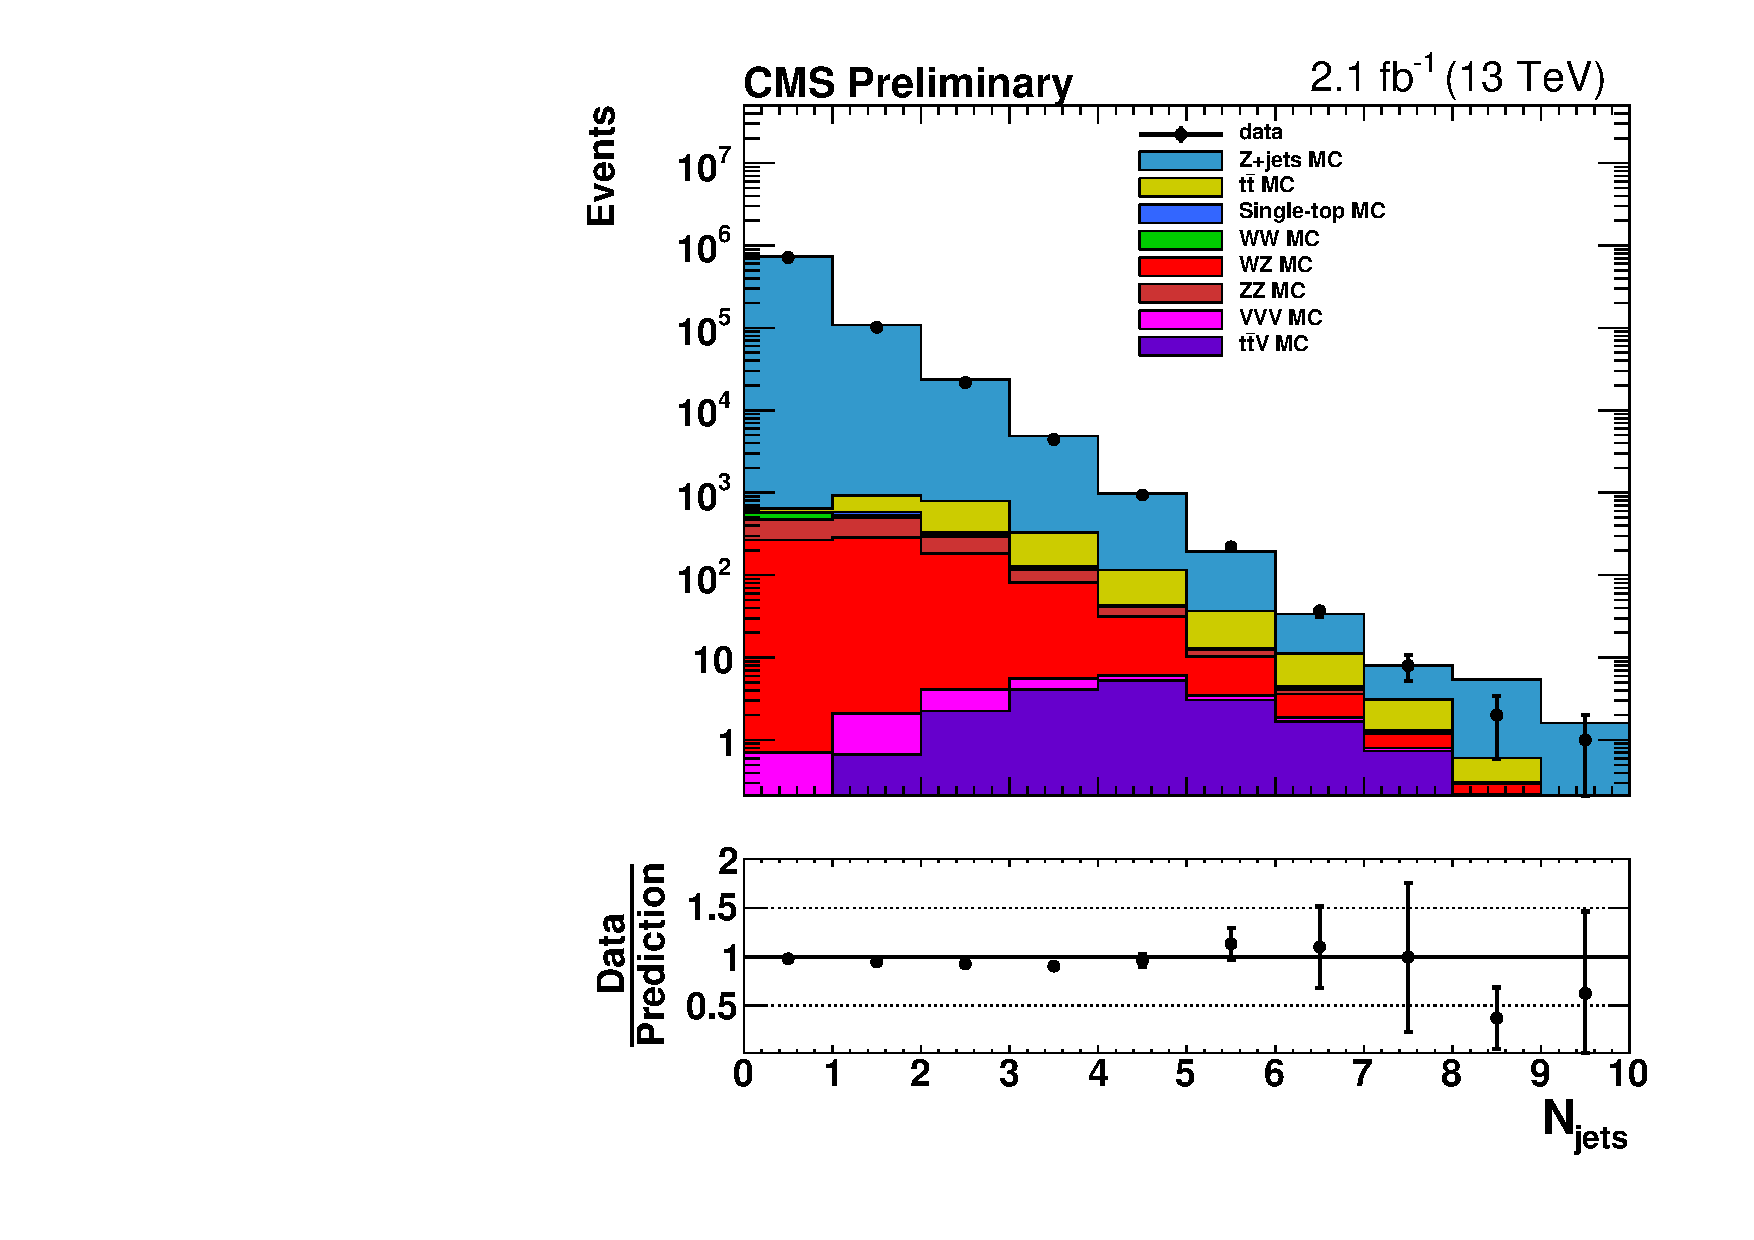
\includegraphics[width=0.4\linewidth]{evtsel/figs/h_njets_ee_signalregion_inclusive_passtrig.pdf} &
      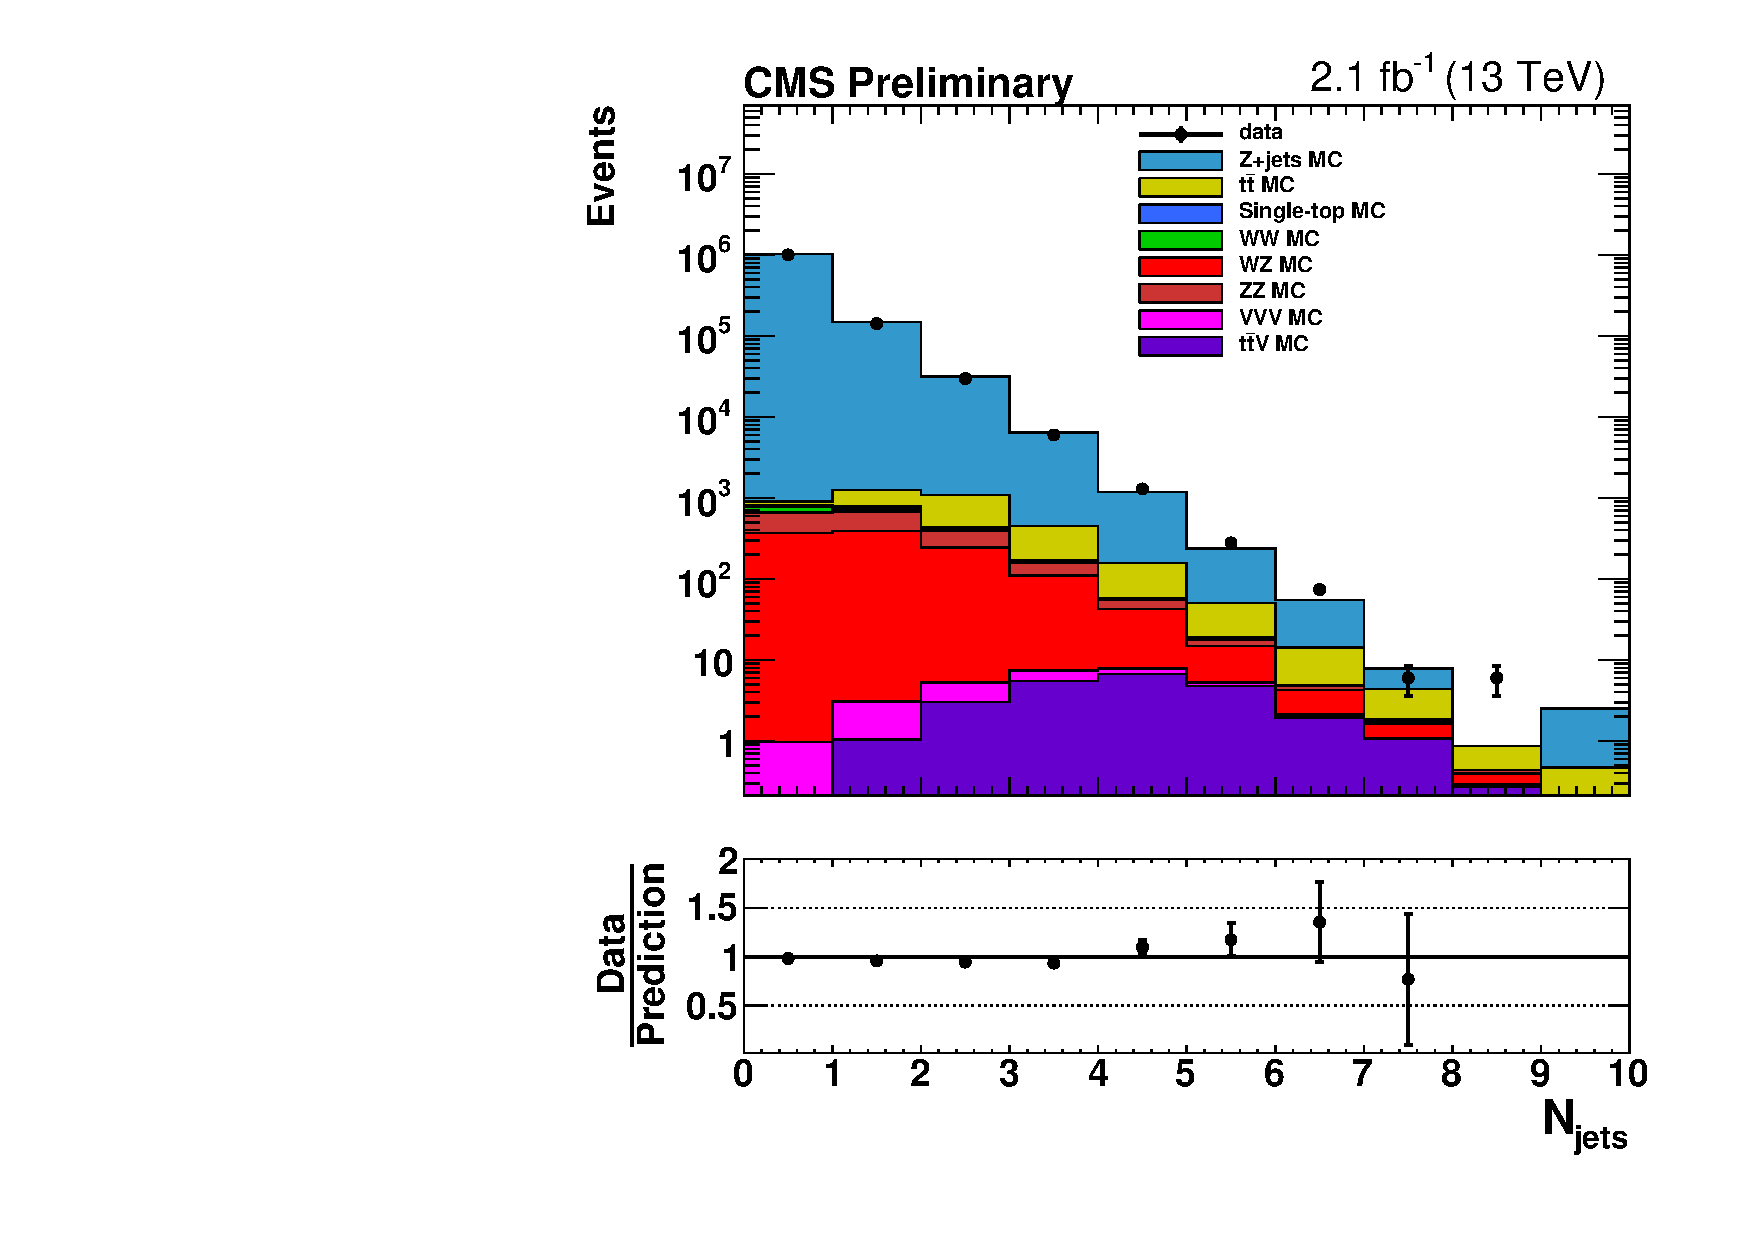
\includegraphics[width=0.4\linewidth]{evtsel/figs/h_njets_mm_signalregion_inclusive_passtrig.pdf} \\
    \end{tabular}
    \caption{
      \label{fig:datavsmc_njets}
      data vs. MC comparison showing $\mathrm{N_{jets}}$ with ee events on the left and $\mu\mu$~events on the right.
    }
  \end{center}
\end{figure}

\begin{figure}[!ht]
  \begin{center}
    \begin{tabular}{cc}
      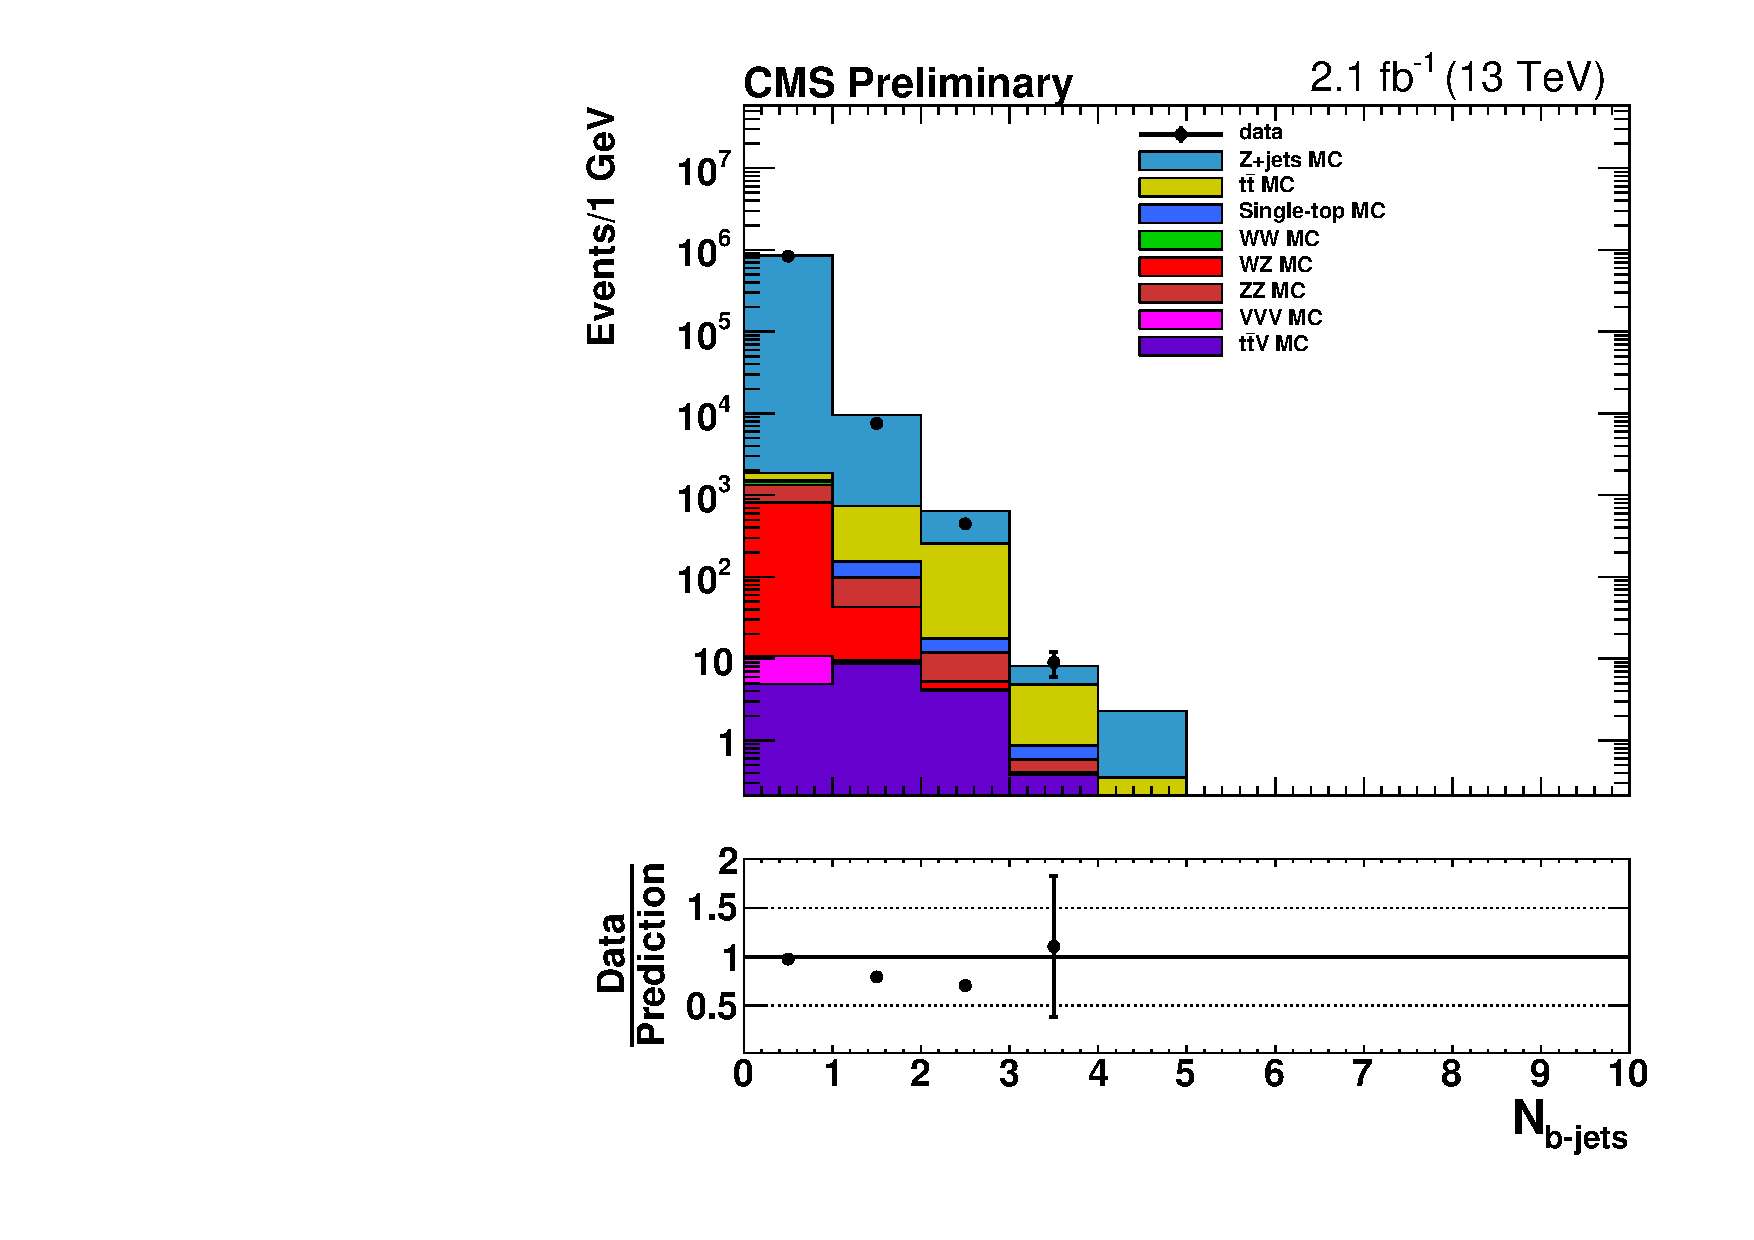
\includegraphics[width=0.4\linewidth]{evtsel/figs/h_nbjets_ee_signalregion_inclusive_passtrig.pdf} &
      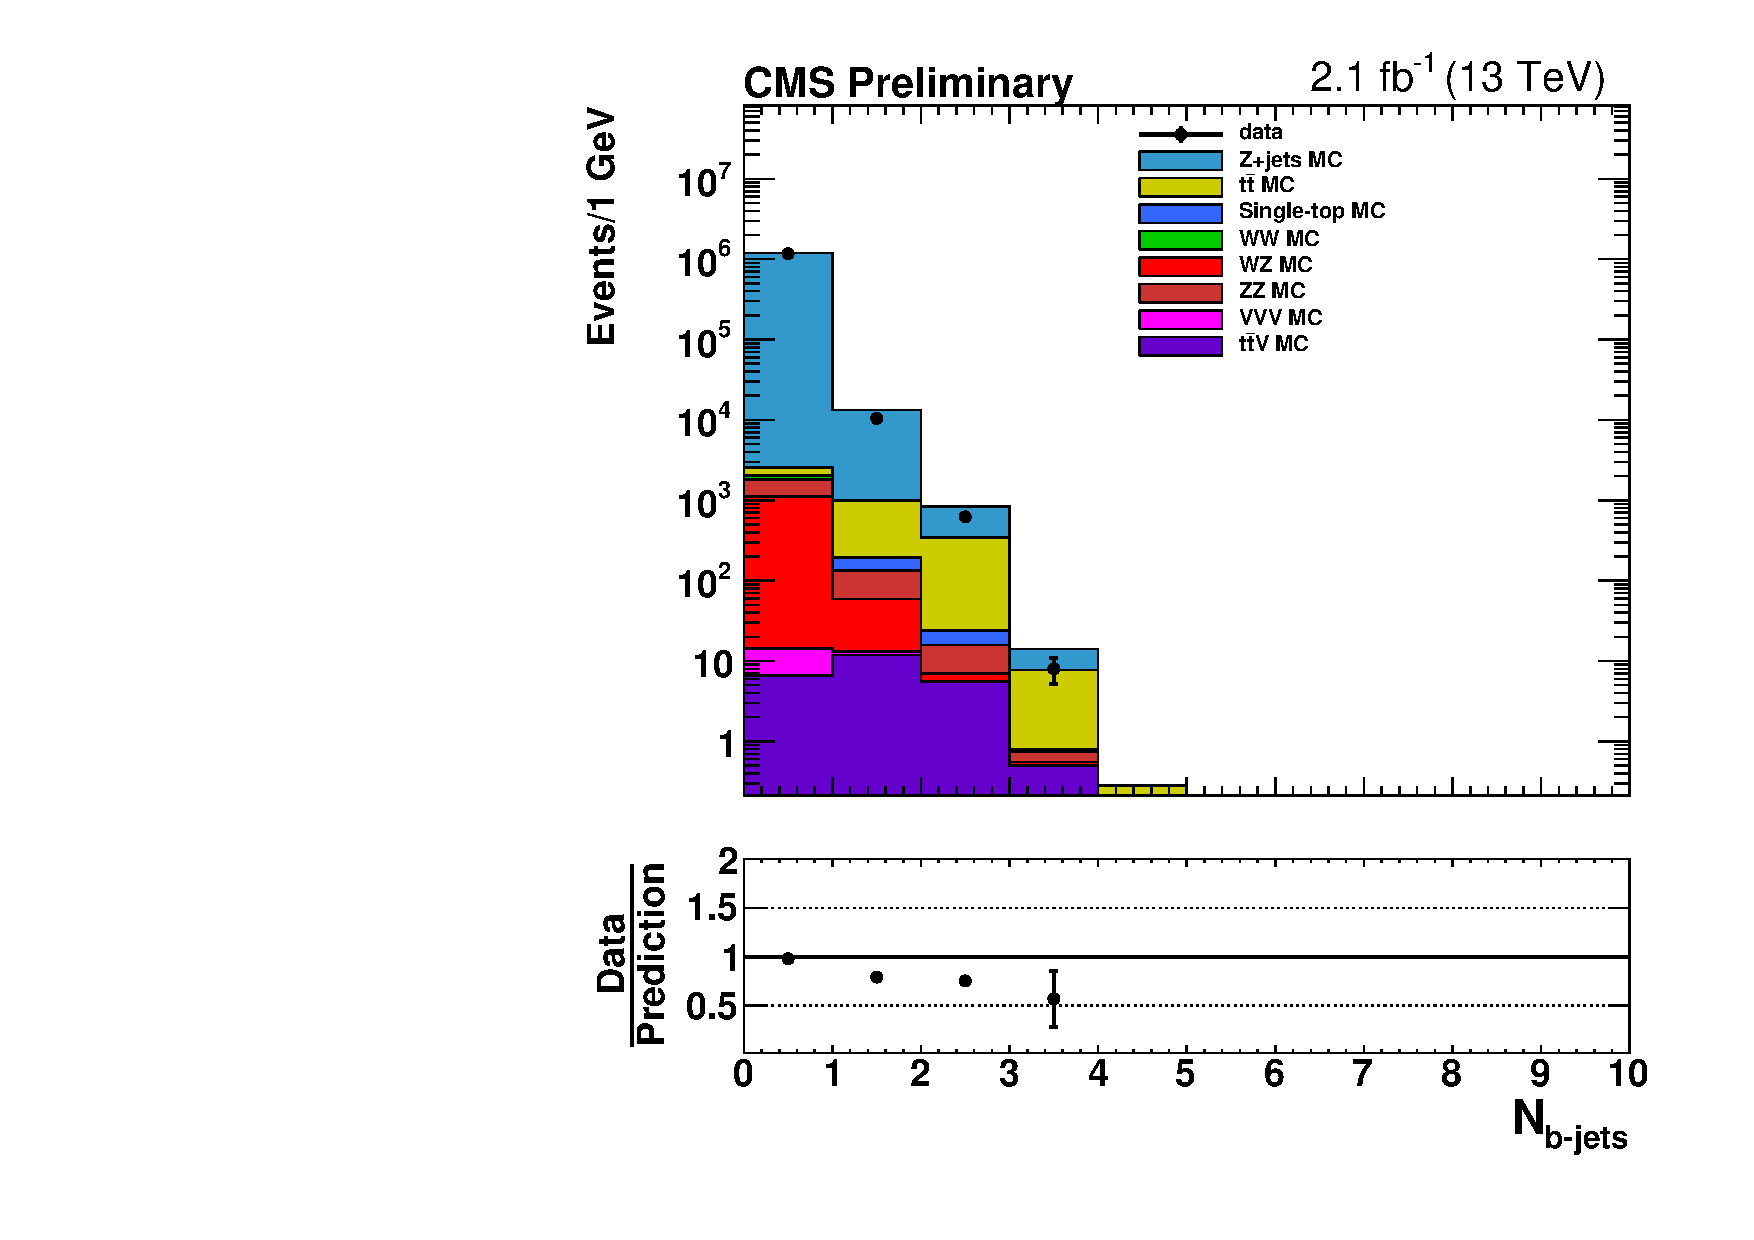
\includegraphics[width=0.4\linewidth]{evtsel/figs/h_nbjets_mm_signalregion_inclusive_passtrig.pdf} \\
    \end{tabular}
    \caption{
      \label{fig:datavsmc_nbjets}
      data vs. MC comparison showing $\mathrm{N_{b-jets}}$ with ee events on the left and $\mu\mu$~events on the right.
    }
  \end{center}
\end{figure}

\begin{figure}[!ht]
  \begin{center}
    \begin{tabular}{cc}
      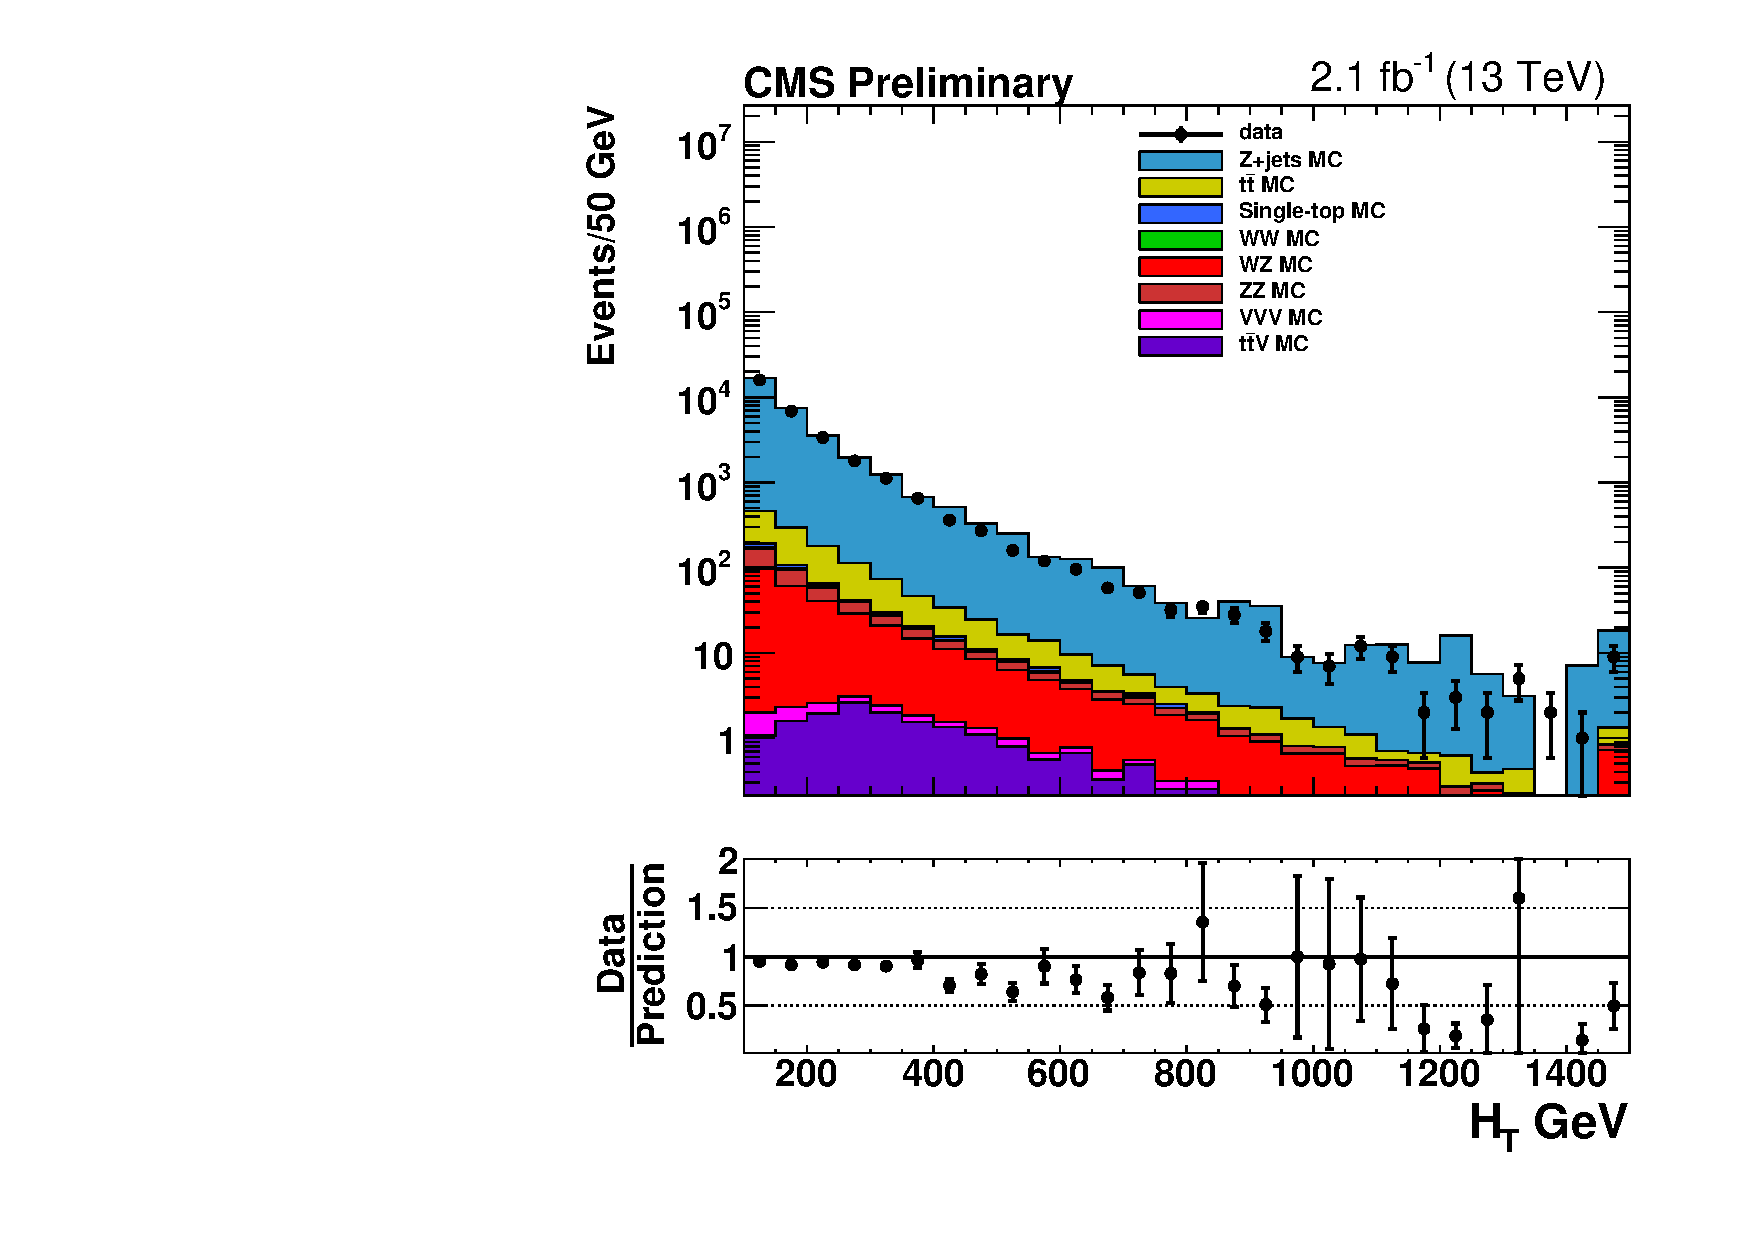
\includegraphics[width=0.4\linewidth]{evtsel/figs/h_ht_highbin_ee_signalregion_inclusive_passtrig.pdf} &
      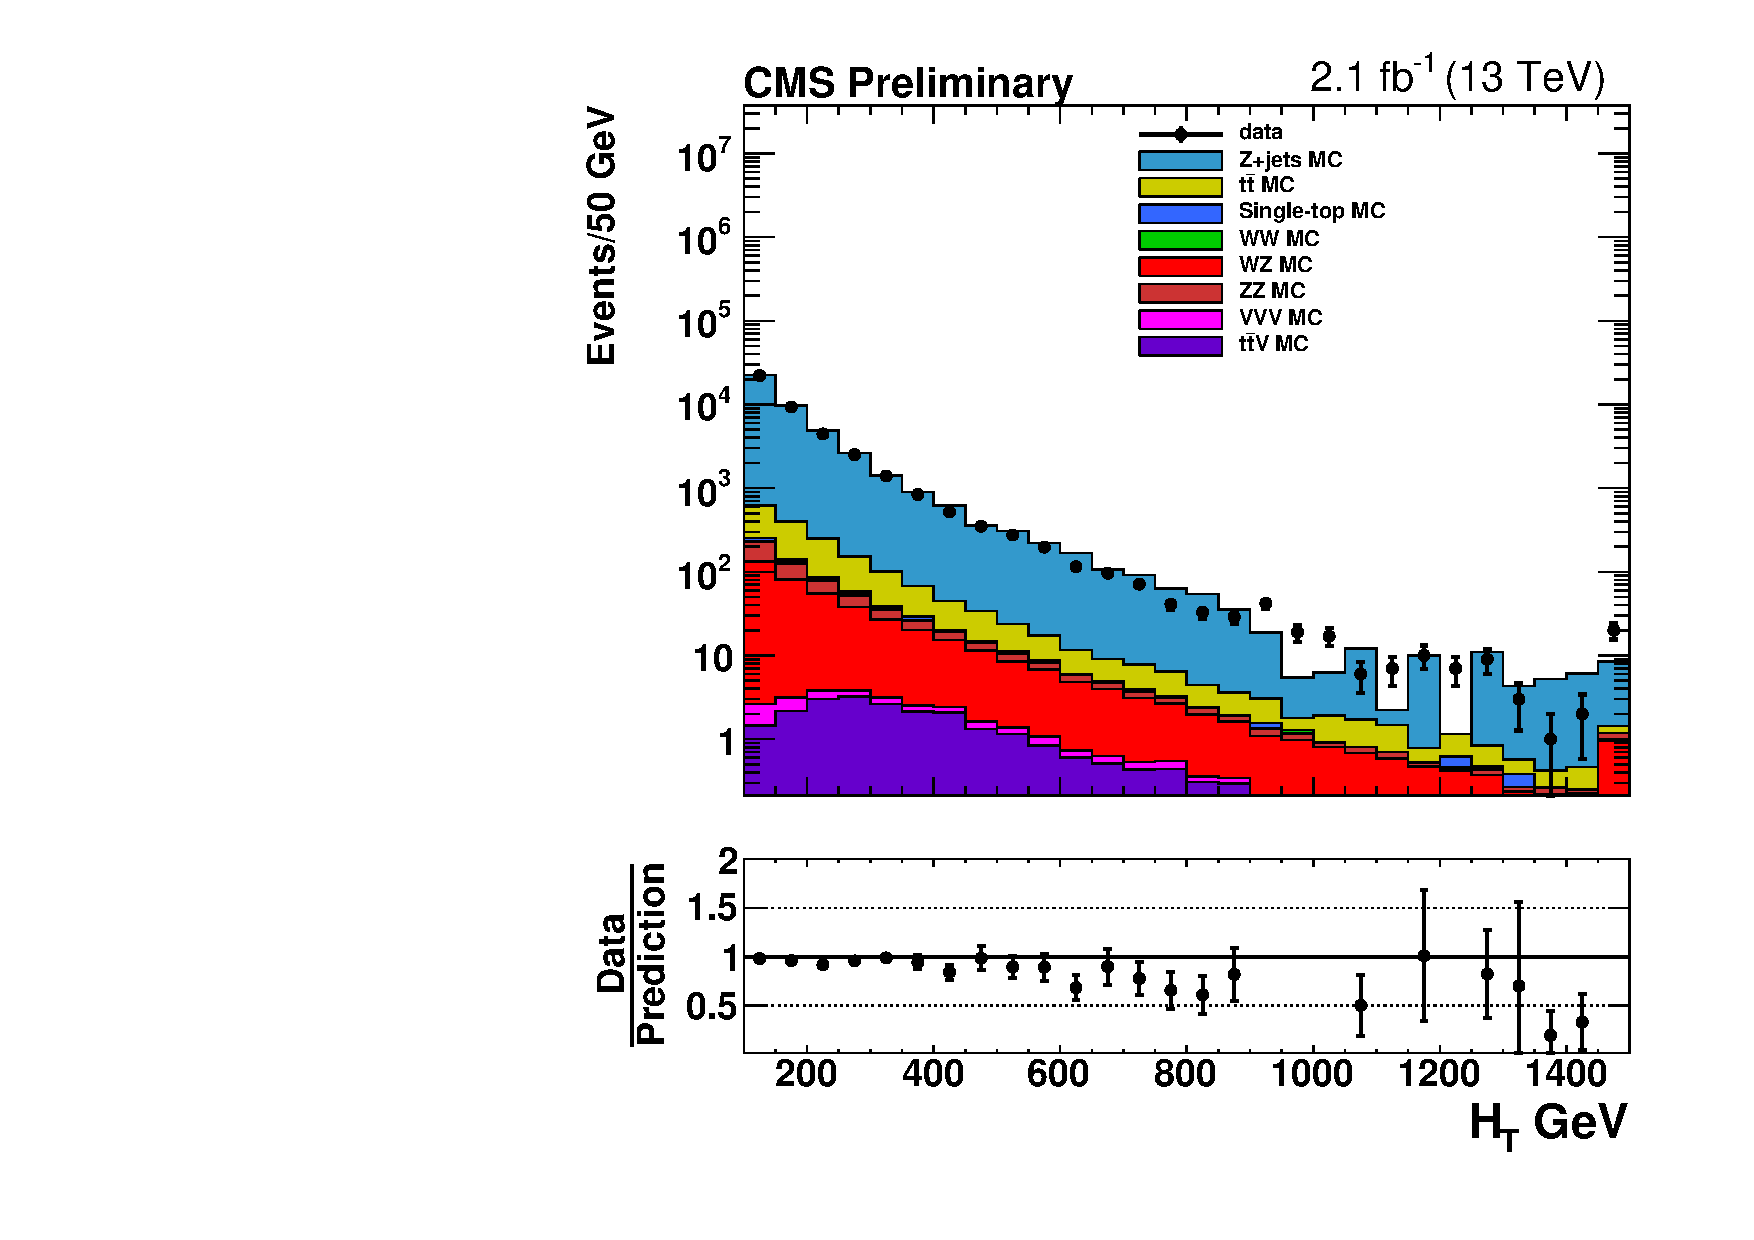
\includegraphics[width=0.4\linewidth]{evtsel/figs/h_ht_highbin_mm_signalregion_inclusive_passtrig.pdf} \\
    \end{tabular}
    \caption{
      \label{fig:datavsmc_ht}
      data vs. MC comparison showing \HT\ with ee events on the left and $\mu\mu$~events on the right.
    }
  \end{center}
\end{figure}

\begin{figure}[!ht]
  \begin{center}
    \begin{tabular}{cc}
      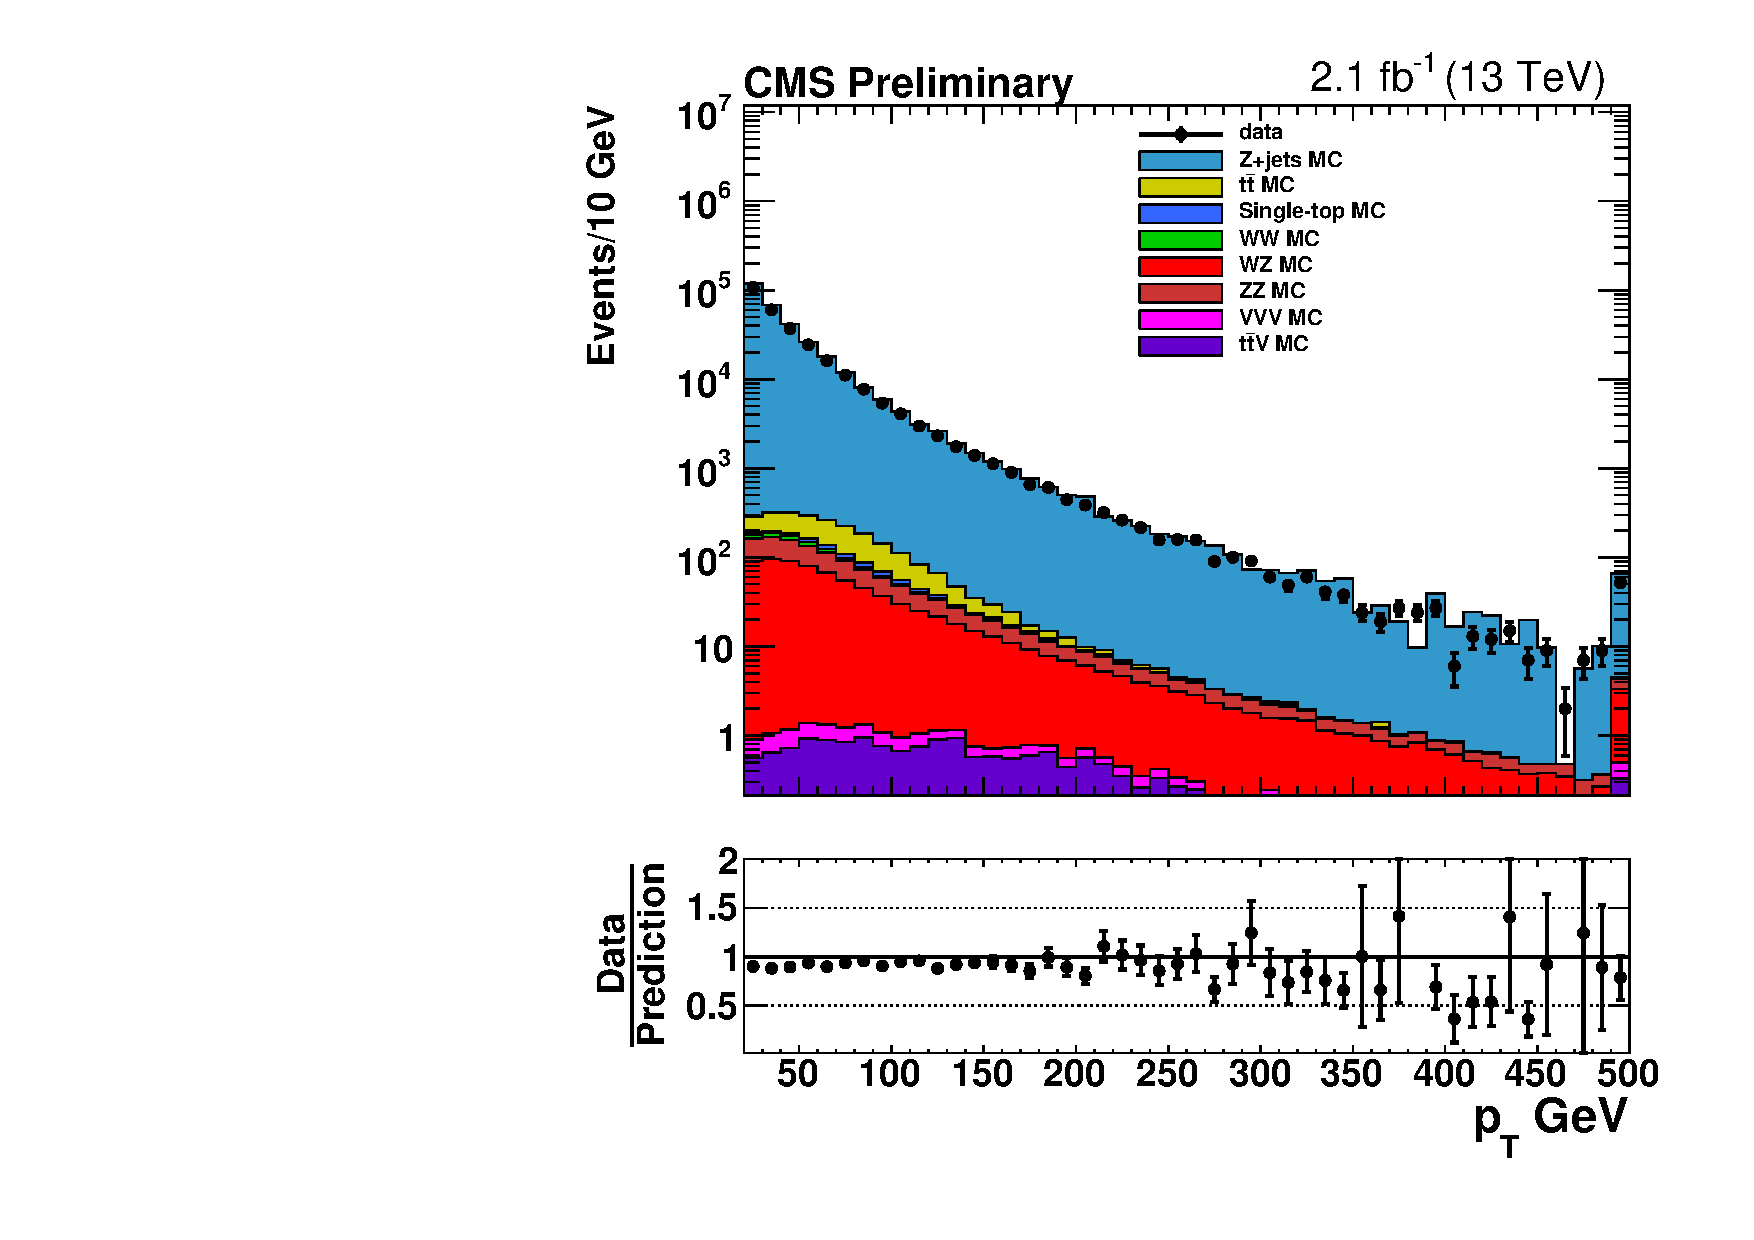
\includegraphics[width=0.4\linewidth]{evtsel/figs/h_ptdil_ee_signalregion_inclusive_passtrig.pdf} &
      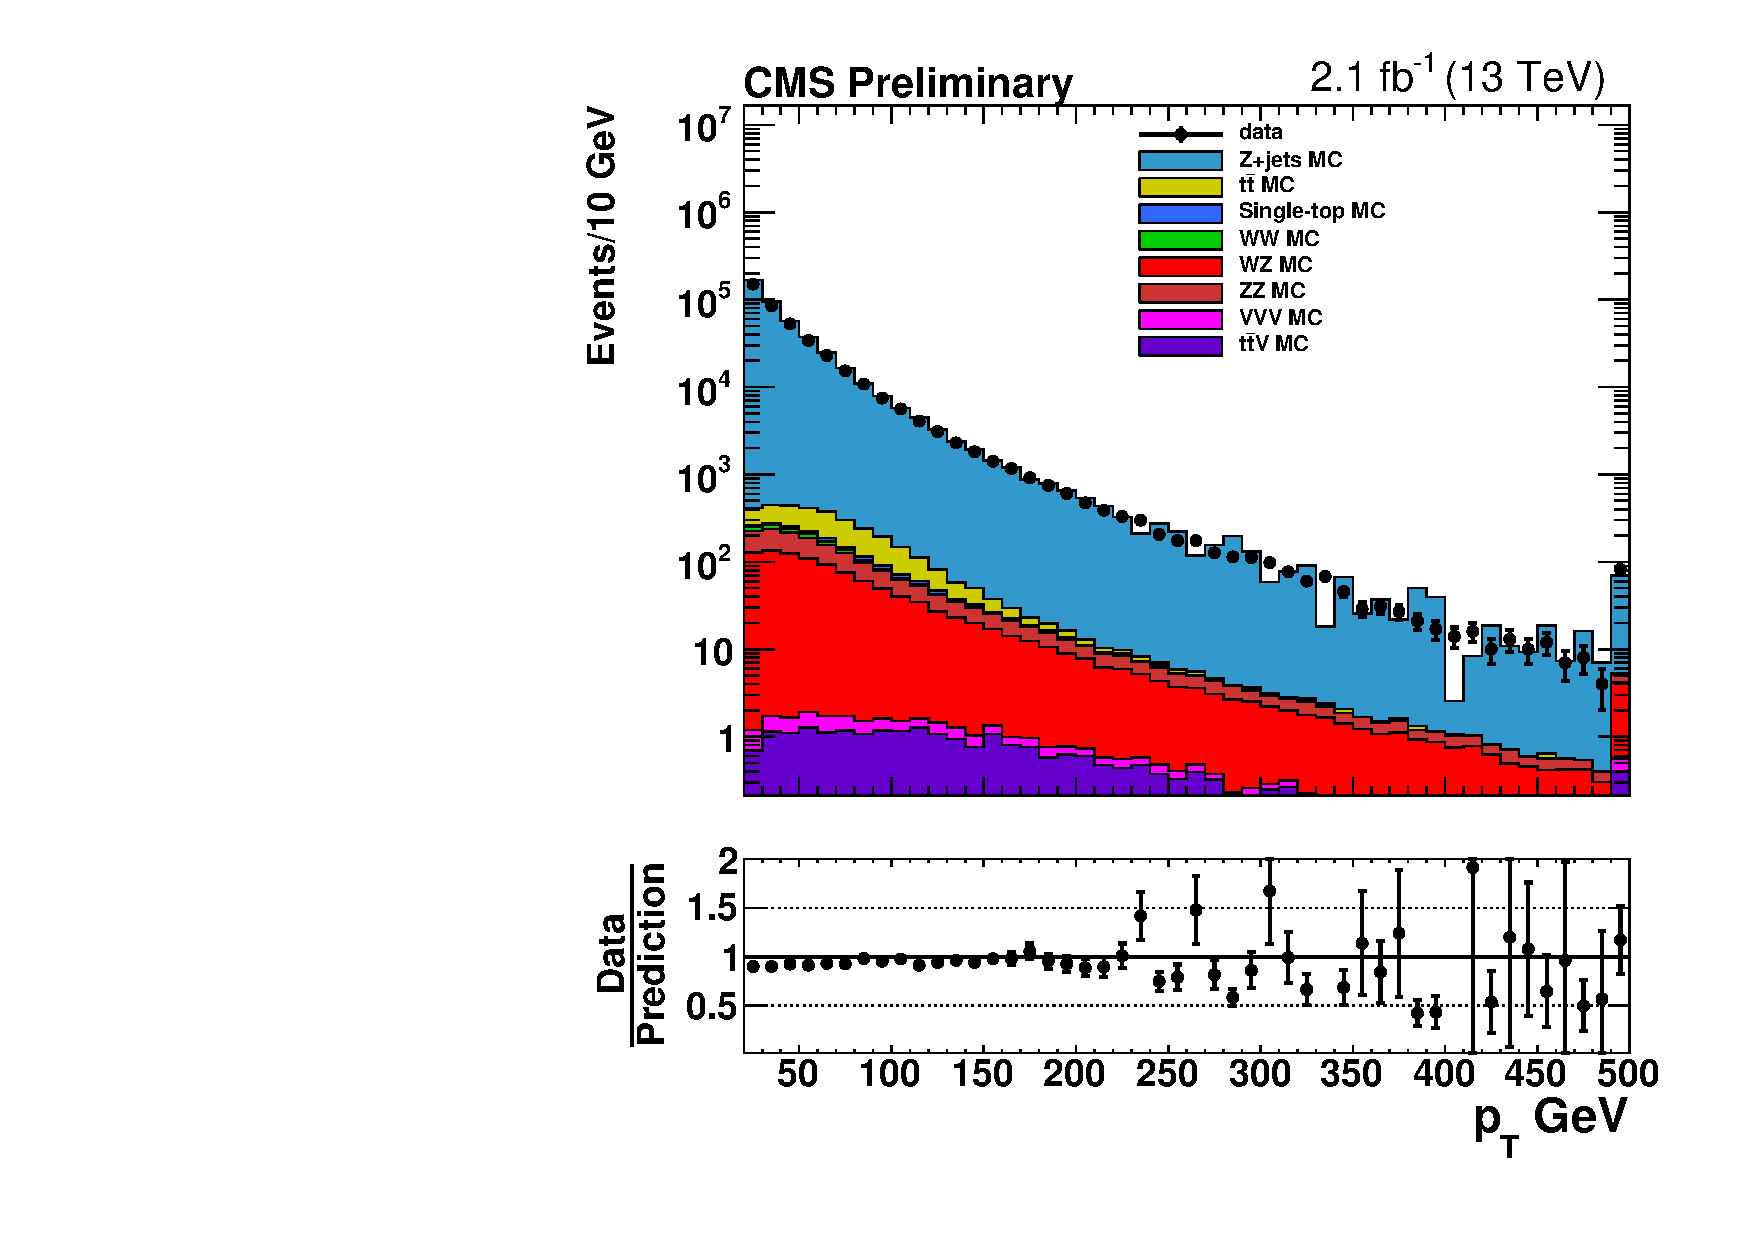
\includegraphics[width=0.4\linewidth]{evtsel/figs/h_ptdil_mm_signalregion_inclusive_passtrig.pdf} \\
    \end{tabular}
    \caption{
      \label{fig:datavsmc_ptdil}
      data vs. MC comparison showing Z \pt\ with ee events on the left and $\mu\mu$~events on the right.
    }
  \end{center}
\end{figure}

\clearpage

\section{Event Selection}
The object selections in this analysis are based on recommendations made by the relevant physics object groups (POGs) in CMS.
These groups are responsible for providing analyzers using data from the CMS experiment with a guideline of how to select specific objects in the event.
These object selections are presented to the experiment as a whole and approved before being commissioned.
In the following sections, the specific object and event selections used in this analysis are described in detail.

\subsection{Vertex Selection}
The method to choose the primary vertices in the event is described in section~\ref{ssec:vtxandpileup}.
For every event, we require the presence of at least one primary vertex satisfying the following criteria:

\begin{itemize}
\item vertex is not fake; \# of degrees of freedom($\mathrm{ndf}$)$>4$; quality requirement
\item $\rho<2$ cm \&\ $|z|<24$ cm; require vertex is inside tracker volume
\end{itemize}

$\rho$ is the radial distance from the center of the beam spot,
and $|z|$ is the distance along the beam direction calculated from the center of the beam spot.

\subsection{MET filters}
\label{ssec:metfilter}
A set of filters designated ``\MET\ filters'' are used in this analysis,
where these filters are designed to remove events in data where large values of \MET\
occur that can come from effects such as noise in the detector or the reconstruction algorithm failing.
The first of these is simply a requirement that at least one good primary vertex is reconstructed in the event.
The next filter is designed to remove events where hits are left in the CSC due to ``beam halo'' effects.
Beam halo is cause by radiation coming from the interactions with the beam in the beam pipe before the beams are collided inside the detector volume.
Additionally, a filter is appplied to deal with energy spikes in the HCAL.
These spikes come from beam halo effects where particles interact with the HCAL in a direction along the beamline leaving large energy signatures.
A filter is then applied for situations where the ECAL readout is saturated.
This happens in regions of the ECAL where there is no coverage due to bad crystals or lack of crystals.
In these regions, the trigger readout is still available but saturates above a certain energy.
When the trigger readout is saturated and the \MET\ vector aligns with an ECAL object in $\phi$, these events are removed.
The next filter applied has to do with known regions in the ECAL where the crystals were previously shown to give incorrect measurements in an incosistent way.
When events have large energies in any of these regions aligned with \MET, the event is filtered.
The last filter has to do with muon reconstruction.
Muons are reconstructed using hits in the muon chamber and matching them with tracks in the tracker.
When a low quality muon is reconstructed,
there is a non-negligible chance for the muon to be matched incorrectly in such a way that gives a large \pt\ value,
which then translates to large \MET.

\subsection{Lepton Selection}
\label{ssec:lepsel}
The goal of this analysis is to study events with a Z boson that decays leptonically,
and we consider only events with Z$\rightarrow\ell\ell$, where $\mathrm{\ell=e~or~\mu}$.
$\tau$s are not considered for reasons described in~\ref{ssec:lepsandphots}.
In order to select events with this decay,
it is required there be at least two leptons passing the ID and isolation requirements described below,
and that these leptons form a opposite-sign same-flavor (OSSF) pair with \mll\ between 81-101 \gev.
When more than one good OSSF di-lepton pair passes all the lepton requirements,
the pair consisting of the two highest \pt\ leptons is chosen.
The two highest \pt\ leptons in the event are required to have \pt\ $> 20$ \gev.
This requirement is chosen based on the expected di-lepton trigger \pt\ thresholds.
In order to have high precision when identifying and reconstructing leptons,
the leptons are required to be contained within the tracker volume.
This is done by requiring both leptons to have $|\eta| < 2.4$.
In order to avoid the transition region from the endcap to the barrel, 
where the muon and electron reconstruction efficiencies are very different, 
leptons having $|\eta|$ in the range 1.4 $< |\eta| <$ 1.6 are rejected.
Events are vetoed if the two leading leptons are within a cone of $\Delta R < 0.1$ from eachother,
in order to reduce the rate of events with fake leptons.
These selections are summarized below.

\begin{itemize}
\item Require two leading leptons to be opposite-sign same-flavor (OSSF) ee and $\mu\mu$ pairs
\item The dilepton invariant mass is required to be consistent with the Z mass; namely $81<m_{\ell\ell}<101$~\gev
\item \pt\ $> 20$ \gev\ for the two leptons making up the di-lepton pair
\item $|\eta| < 1.4$~or $1.6 < |\eta| < 2.4$~for the two leptons making up the di-lepton pair
\item $\Delta R$~between the two leading leptons must be greater than 0.1
\end{itemize}

\subsection{Lepton Isolation}
\label{ssec:isolation}
The signal region targeted by this analysis is expected to have large \HT\ due to the many jets in the final state.
This leads to an increased probability of a lepton overlapping with a jet in the event.
When this happens, the lepton is no longer isolated and may fail a cut on the raw isolation value.
The isolation variable is designed to reduce this inefficiency by using a variable cone size that depends on lepton \pt.
For leptons with \pt\ $<$~50 \gev, we use a cone with $\Delta\mathrm{R = 0.2}$,
for leptons with \pt: 50 - 200 \gev, we use a variable cone defined as $\Delta\mathrm{R = \frac{10}{p_{T}(lep)}}$,
and for leptons with \pt $>$~200 \gev, we use a cone with $\Delta\mathrm{R = 0.05}$.
Isolation is calculated according to equation~\ref{eqn:isolation},
where $\mathrm{p_{T}(i)}$~represents all the pf candidates within the cone defined above.
When cutting on isolation, the value is chosen relative to $\mathrm{p_{T}(lepton)}$. 
This quantity is designated mini-relative Isolation (miniRelIso).

\begin{equation}
\label{eqn:isolation}
\mathrm{I_{lepton}} = \sum _{i} |\mathrm{p_{T}(i)| - |p_{T}(lepton)}|
\end{equation}

Before cutting on isolation,
corrections are made to account for pileup energy using the effective area $\rho$ corrections scheme.
In this scheme, $\rho$ is the total energy density from pileup and is assumed to be uniform in the detector.
The correction to isolation is done by calculating the energy from pileup in the isolation cone and subtracting it from the total energy in the cone.

This correction is not derived using the geometric area of the cone however
due to the fact that the response of $I_{lepton}$ and $\rho$ are different with respect to the amount of pileup.
Instead, the geometric area of each lepton's isolation cone is scaled in separate regions of $\eta$
by a factor derived using the number of primary vertices in the event as a way to estimate the amount of pileup.
These factors are derived separately for electrons and muons and shown in tables~\ref{tab:eamus}~and~\ref{tab:eaels}.

\begin{table}[htb]
\begin{center}
  \caption{
    \label{tab:eamus}
    Effective area values for muons derived in separate regions of $\eta$.
  }
\begin{tabular}{l|c}
\hline
\hline
$\eta$~region        & Muon effective area \\
\hline
$|\eta| < 0.8$       & 0.0735 \\
0.8$ < |\eta| < $1.3 & 0.0619 \\
1.3$ < |\eta| < $2.0 & 0.0465 \\
2.0$ < |\eta| < $2.2 & 0.0433 \\
2.2$ < |\eta| < $2.5 & 0.0577 \\
\hline
\hline
\end{tabular}
\end{center}
\end{table}

\begin{table}[htb]
\begin{center}
  \caption{
    \label{tab:eaels}
    Effective area values for electrons derived in separate regions of $\eta$.
  }
\begin{tabular}{l|c}
\hline
\hline
$\eta$~region          & Electron effective area \\
\hline
$|\eta| < 1.0$         & 0.1752 \\
1.0$ < |\eta| < $1.3   & 0.1862 \\
1.479$ < |\eta| < $2.0 & 0.1411 \\
2.0$ < |\eta| < $2.2   & 0.1534 \\
2.2$ < |\eta| < $2.3   & 0.1903 \\
2.3$ < |\eta| < $2.4   & 0.2243 \\
2.4$ < |\eta| < $2.5   & 0.2687 \\
\hline
\hline
\end{tabular}
\end{center}
\end{table}

The effective area is then defined by equation~\ref{eqn:effarea} where f is the scale factor, and R is the cone size defined above.

\begin{equation}
\label{eqn:effarea}
\mathrm{A_{eff} = f*\pi * R^2}
\end{equation}

The plots in figures~\ref{fig:isoels}~and~\ref{fig:isomus}
show the isolation distribution for leptons that pass the ID selections made using simulated \zjets\ MC.
These leptons are separated into two categories, prompt and non-prompt leptons.
Prompt leptons are defined to be leptons that come directly from the hard scatter process rather than a second order process, for example semi-leptonic b-decay.
In order to study the difference in expected behavior of prompt and non-prompt leptons, a disctinction is made such that a prompt,
reconstructed lepton is defined as being matched to a generator-level lepton within a cone of $\Delta$R < 0.4.
Any lepton that passes the ID requirements that does not pass this matching requirement is designated as a non-prompt lepton.

\begin{figure}[!ht]
\begin{center}
\begin{tabular}{cc}
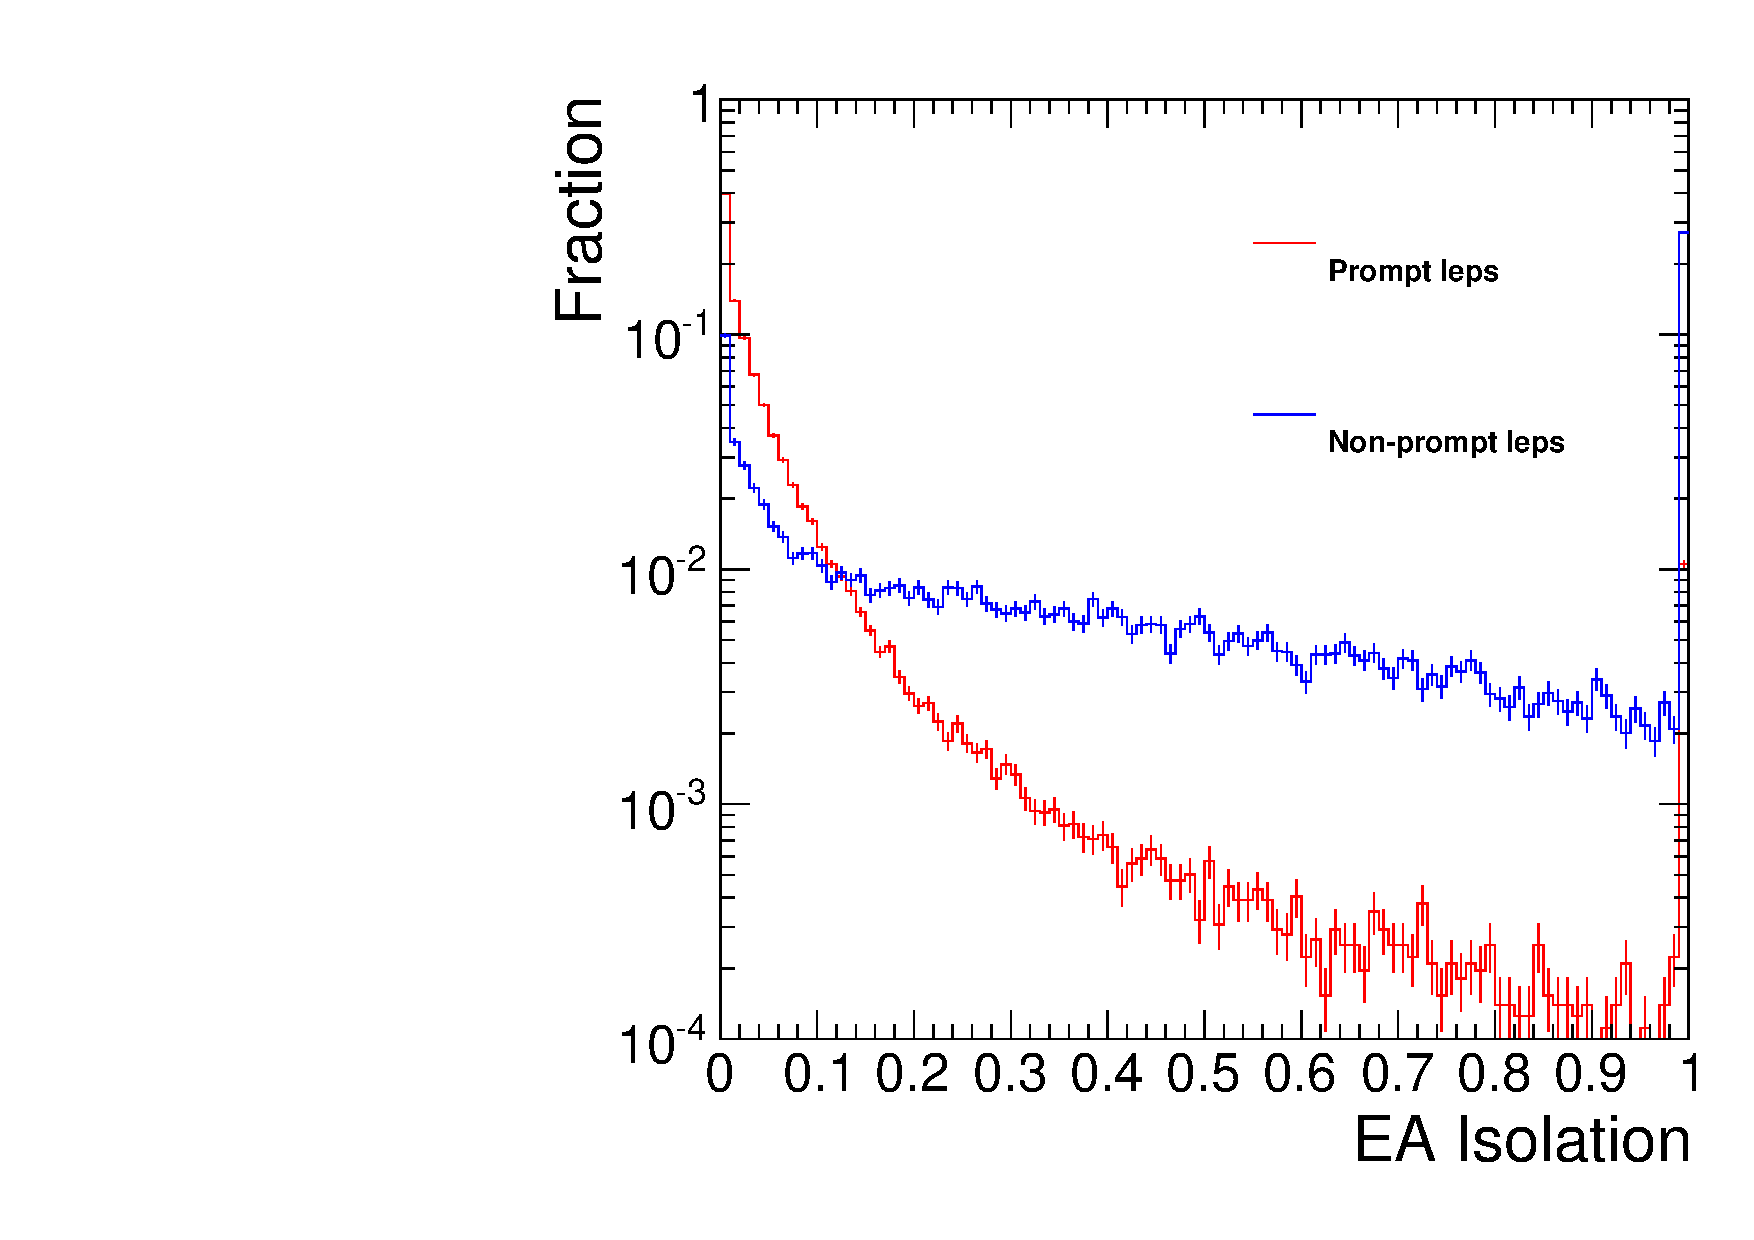
\includegraphics[width=0.4\textwidth]{evtsel/figs/EA_iso_el.pdf} & 
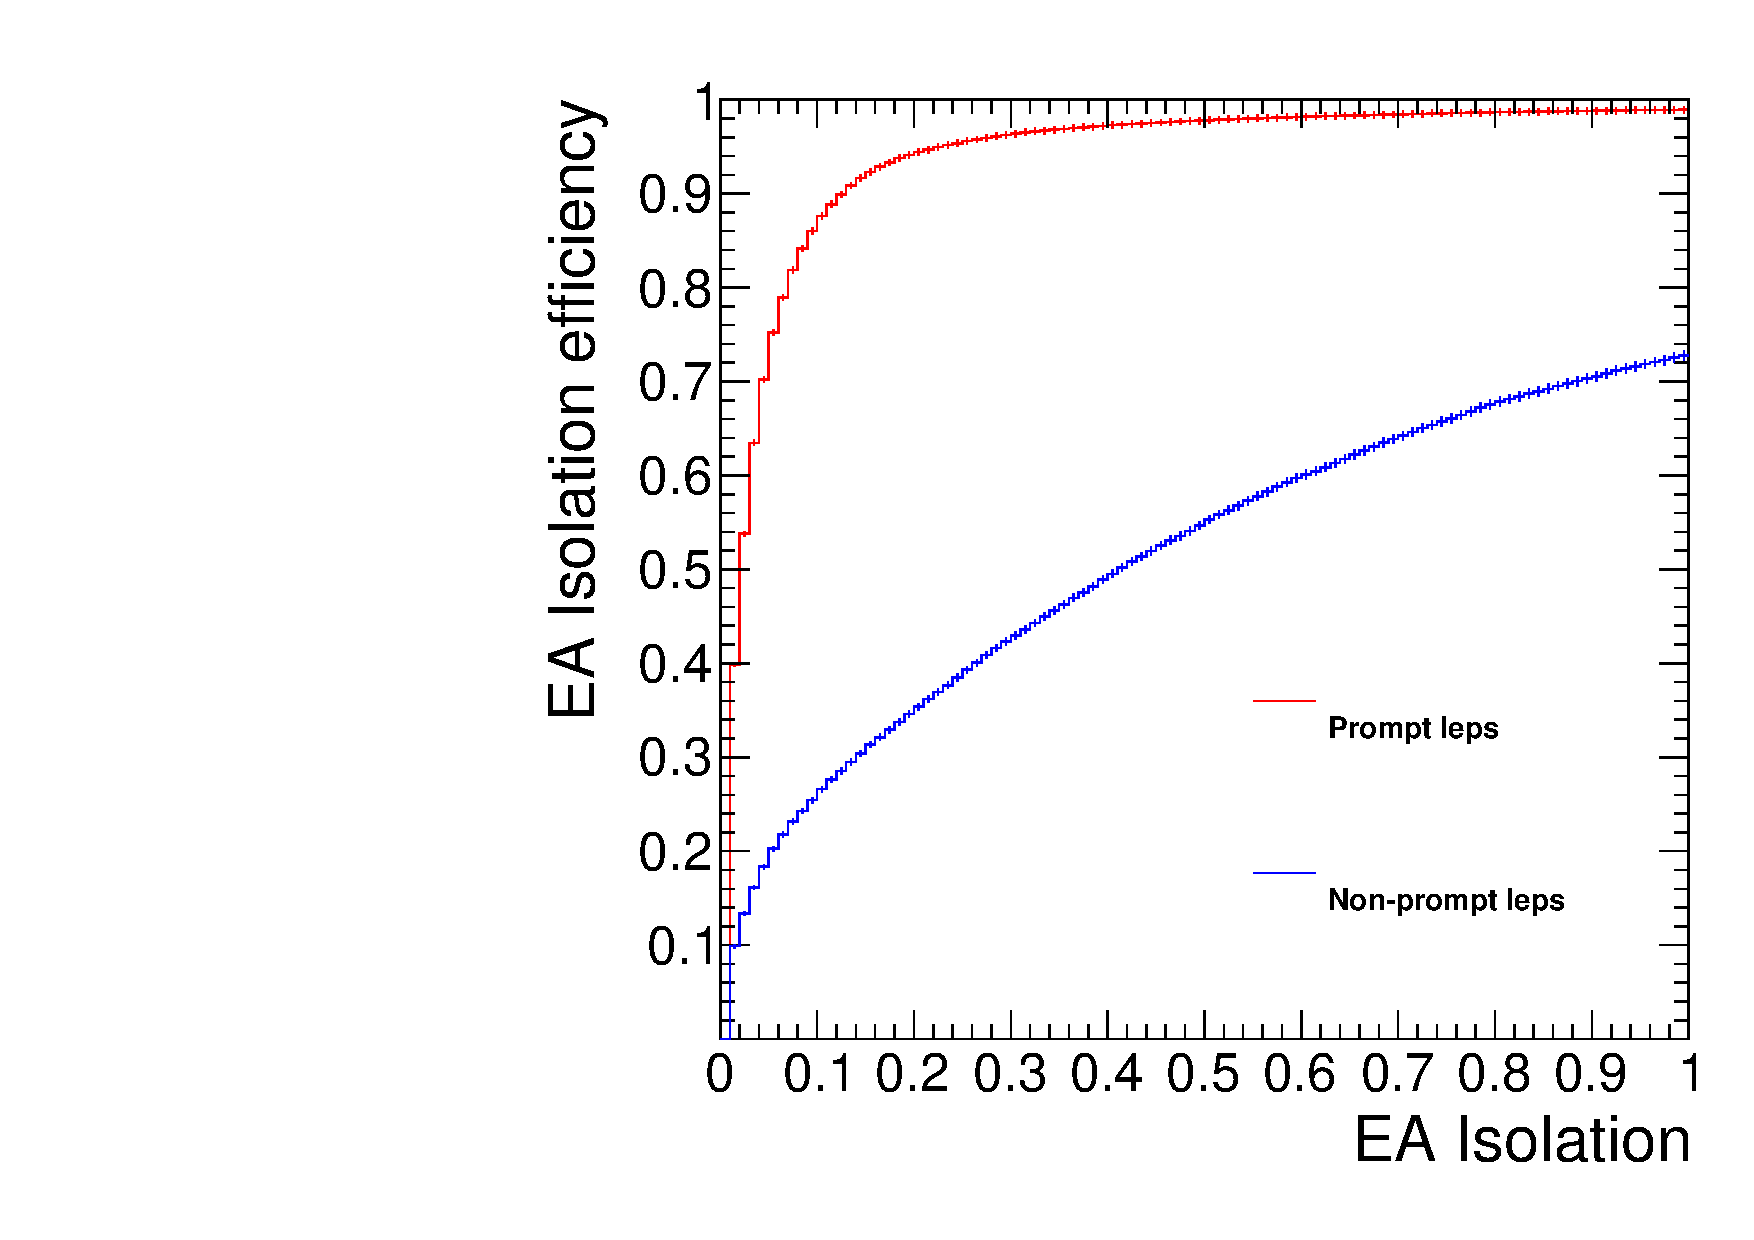
\includegraphics[width=0.4\textwidth]{evtsel/figs/EA_iso_el_inclusive.pdf} \\
\end{tabular}
\caption{
  The isolation distribution is shown for electrons on the left in simulated \zjets\ MC events.
  On the right, the efficiency is shown when integrating all bins to the left of the value on the x-axis.
\label{fig:isoels}
}
\end{center}
\end{figure}

\begin{figure}[!ht]
\begin{center}
\begin{tabular}{cc}
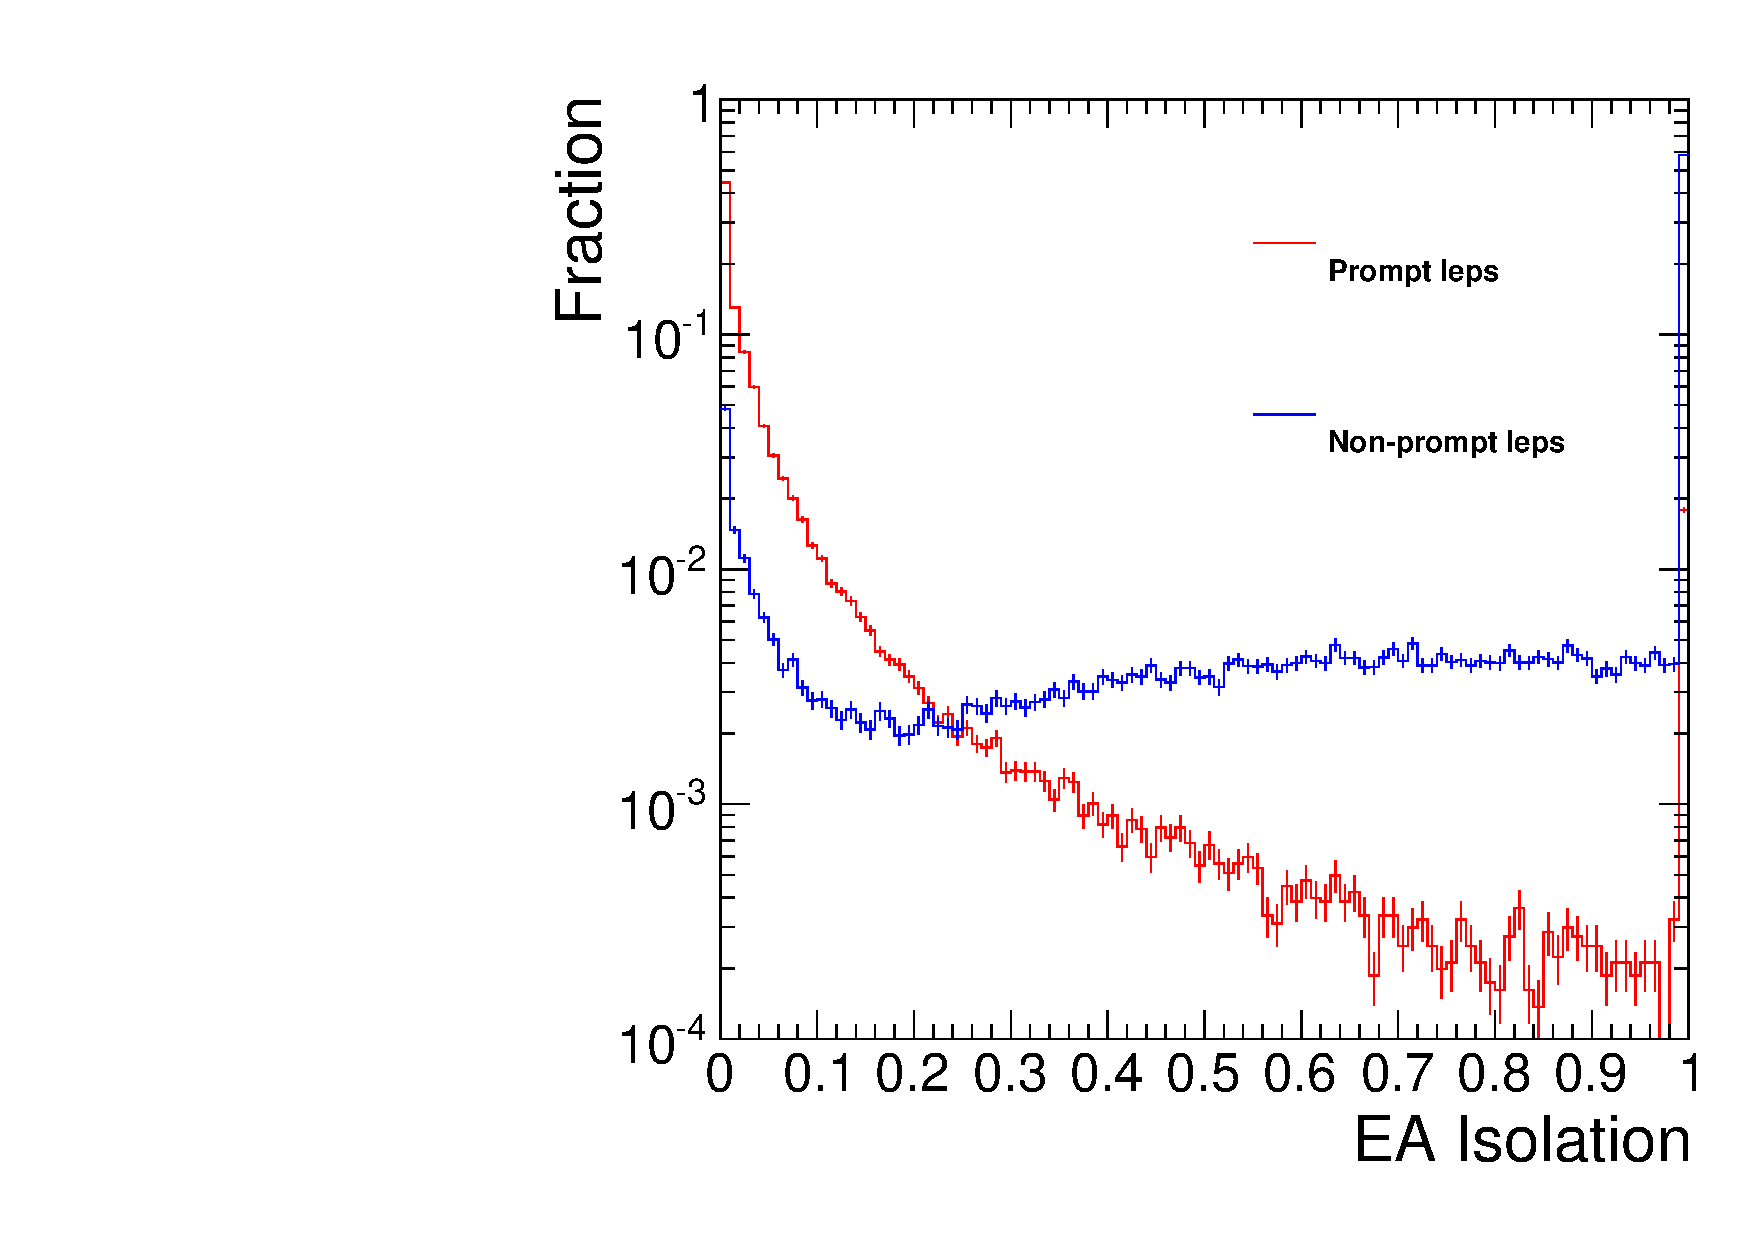
\includegraphics[width=0.4\textwidth]{evtsel/figs/EA_iso_mu.pdf} & 
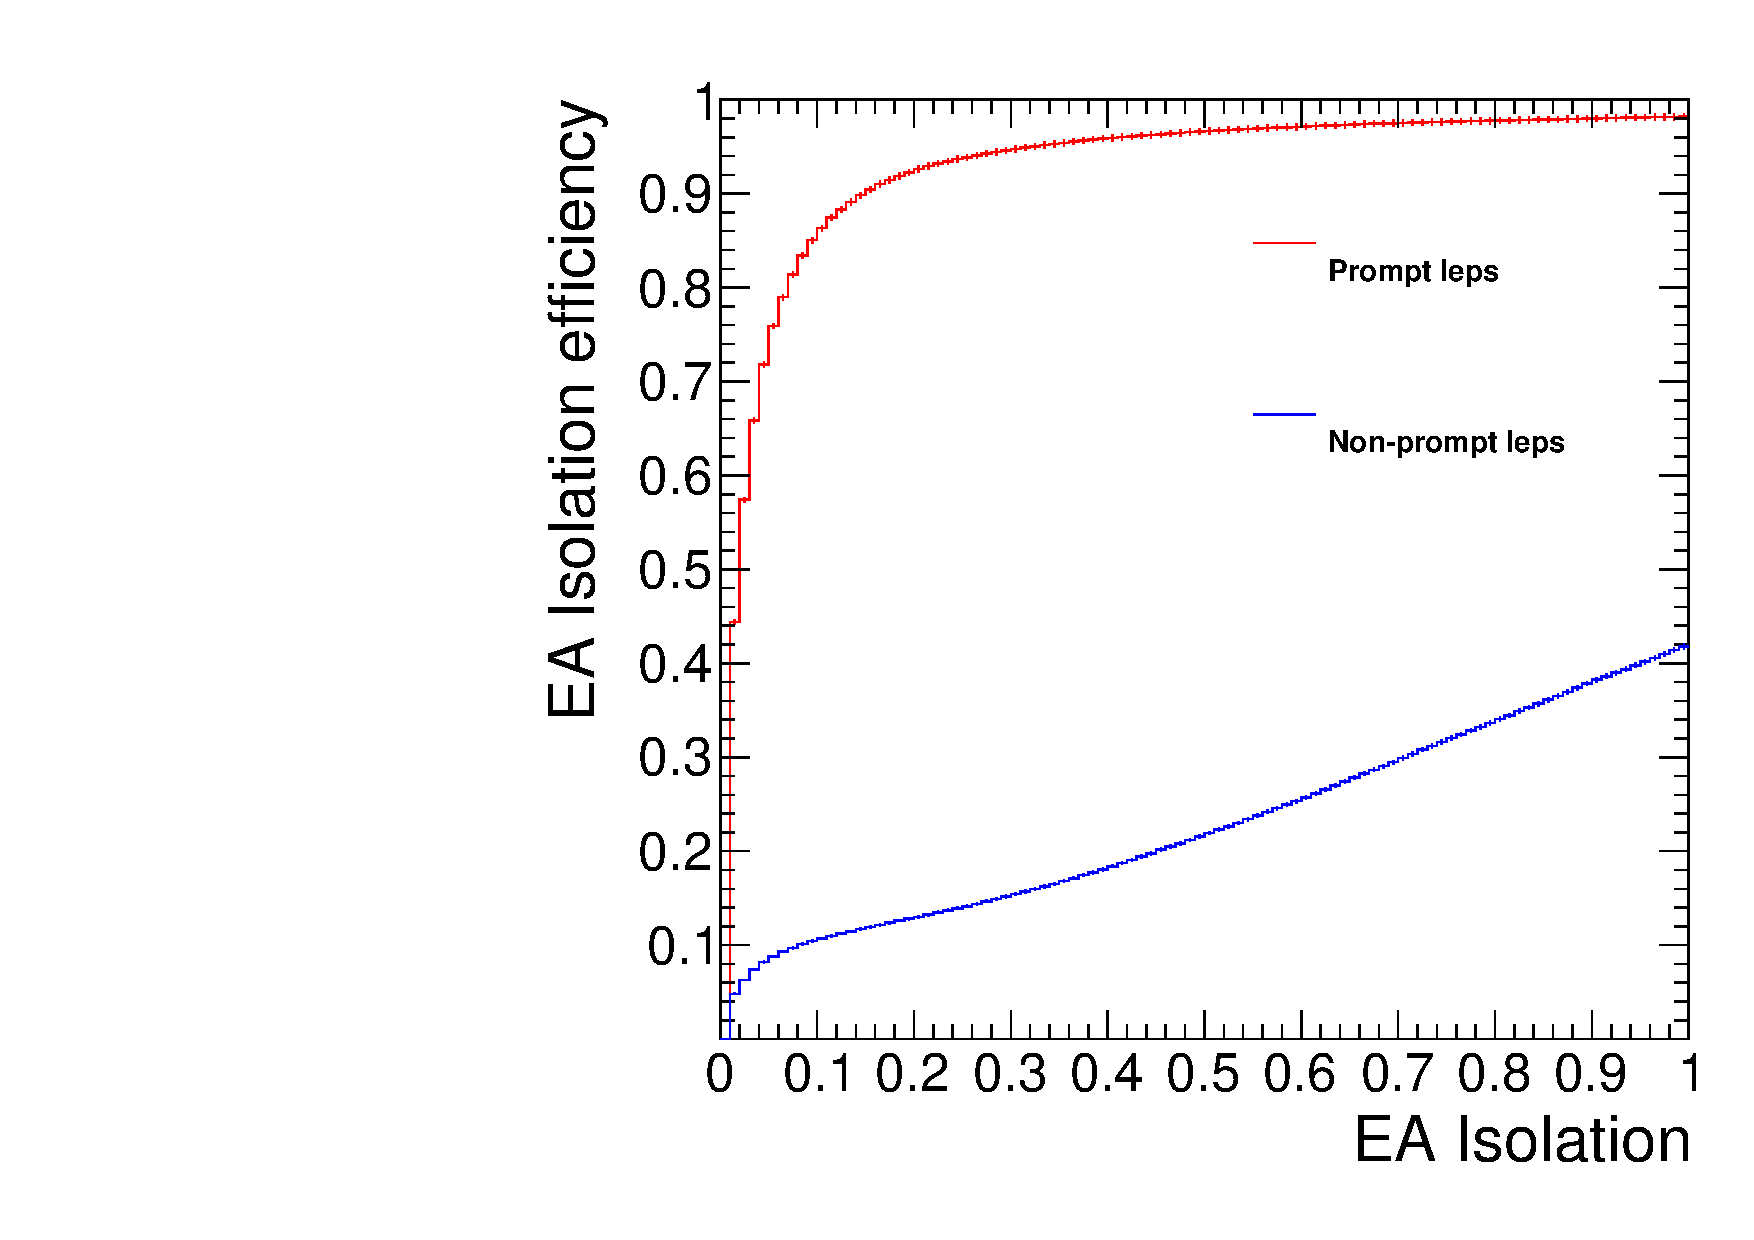
\includegraphics[width=0.4\textwidth]{evtsel/figs/EA_iso_mu_inclusive.pdf} \\
\end{tabular}
\caption{
  The isolation distribution is shown for muons on the left in simulated \zjets\ MC events.
  On the right, the efficiency is shown when integrating all bins to the left of the value on the x-axis.
\label{fig:isomus}
}
\end{center}
\end{figure}

After applying the effective area corrections,
the leptons in this analysis are required to have miniRelIso $<$ 0.10 ( 0.20) for electrons (muons). 
This gives an efficiency for prompt leptons of $>$~90\% and rejection rate for non-prompt leptons of about 80\% for electrons and 90\% for muons.
\clearpage

\subsection{Lepton Scale Factors}
\label{ssec:lepscalefactors}
Scale factors are applied in order to correct for the differences in efficiencies in data and MC when selecting applying lepton ID and isolation requirements.
Additional scale factors are derived to correct for differences in simulation of leptons when using Fastsim~\cite{fastsim} instead of fullsim.
These scale factors are derived in data and MC using a ``tag and probe'' technique.
The main premise of this technique is that leptons coming from a Z boson are produced in opposite-sign same-flavor pairs in very large quantities.
In an event, a lepton with very tight ID and isolation requirements is chosen (the tag),
and then a second lepton with very loose requirements (the probe) can be studied if it is found that the pair of leptons has a dilepton mass consistent with the Z mass.
The efficiency of various kinematic cut requirements can then be assessed on individual leptons, such as the efficiency of the ID and isolation requirements.
This is done separately in data and MC, and then the MC is corrected based on these differences to match what is observed in data.
Scale factors for electron ID and isolation criteria are shown in~\ref{fig:sf_electrons},
scale factors for muon ID and isolation criteria are shown in~\ref{fig:sf_muons},
and Fastsim scale factors are shown in~\ref{fig:FS_sfs}.
\begin{figure}[!ht]
  \begin{center}
      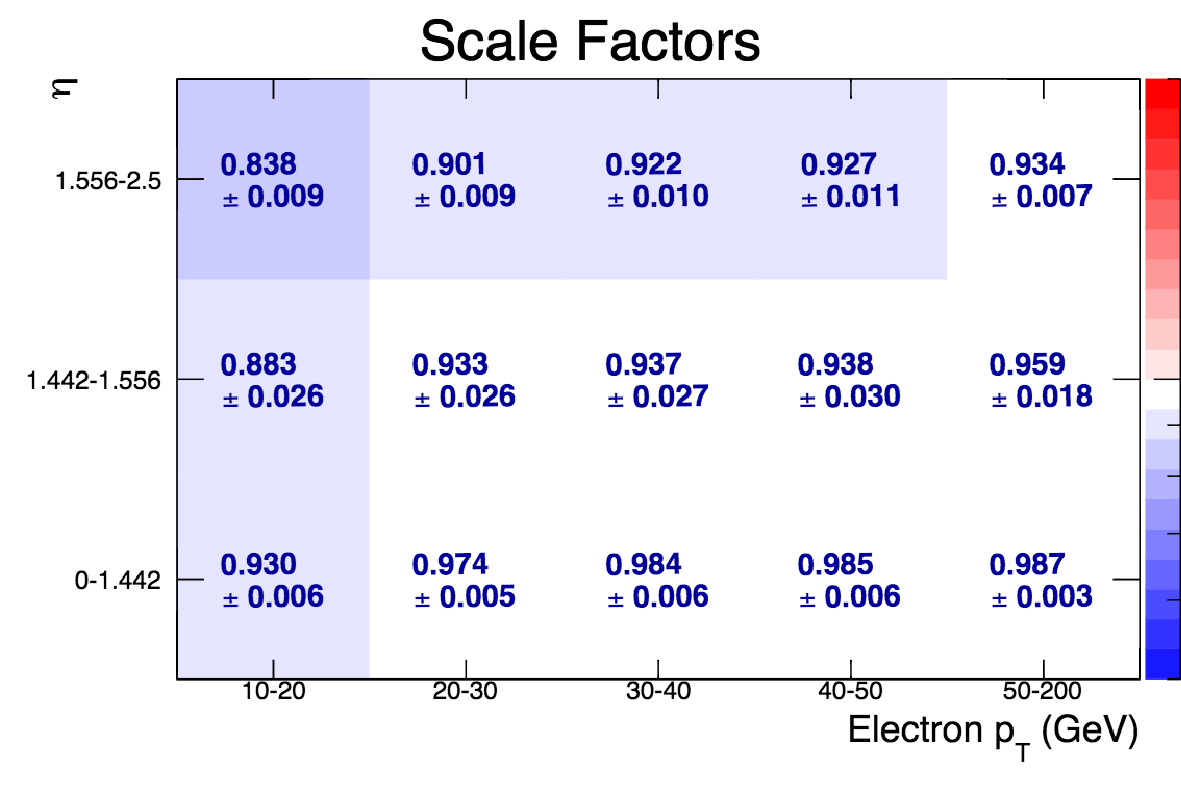
\includegraphics[width=0.8\textwidth]{evtsel/figs/sf_el_tight2d3d.pdf}  
    \caption{
      \label{fig:sf_electrons}
      Electron scale factors as a function of \pt\ and $\eta$.
      The scale factor is applied as an event weight once per electron in the event.
    }
  \end{center}
\end{figure}

\begin{figure}[!ht]
  \begin{center}
    \begin{tabular}{cc}
      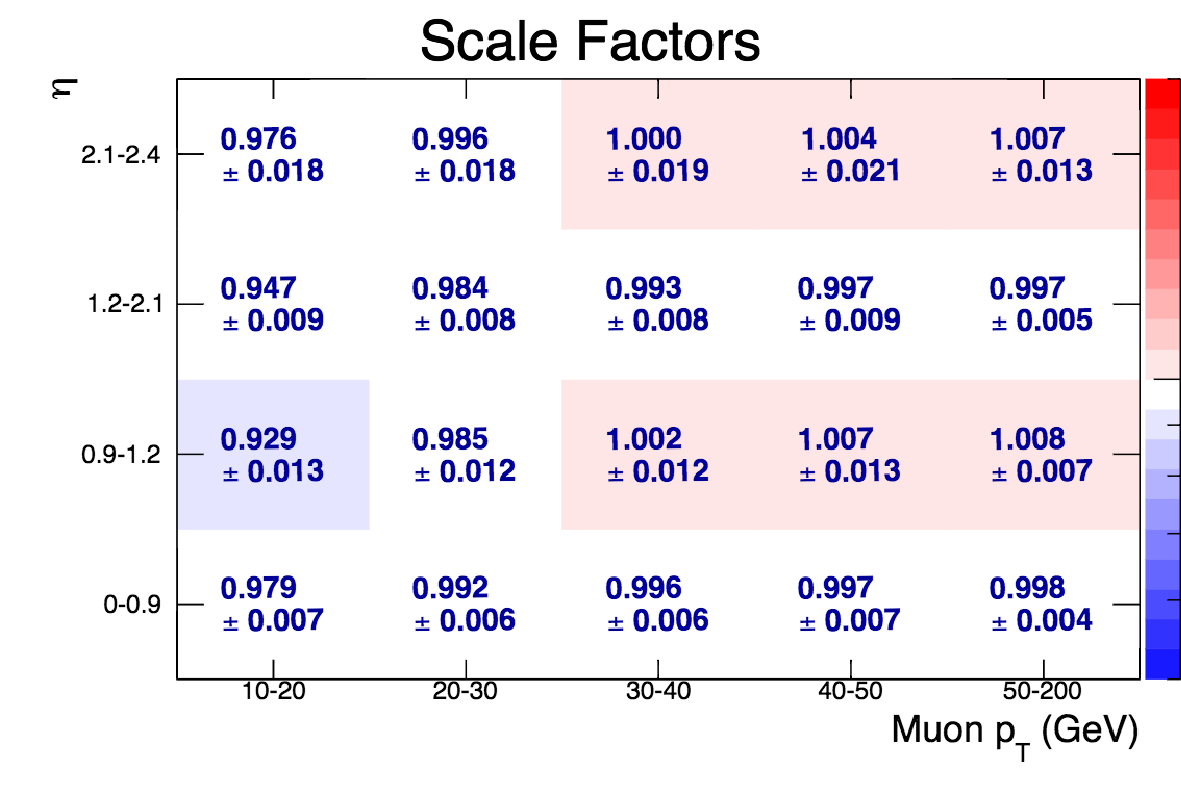
\includegraphics[width=0.4\textwidth]{evtsel/figs/sf_mu_mediumID.pdf}  &
      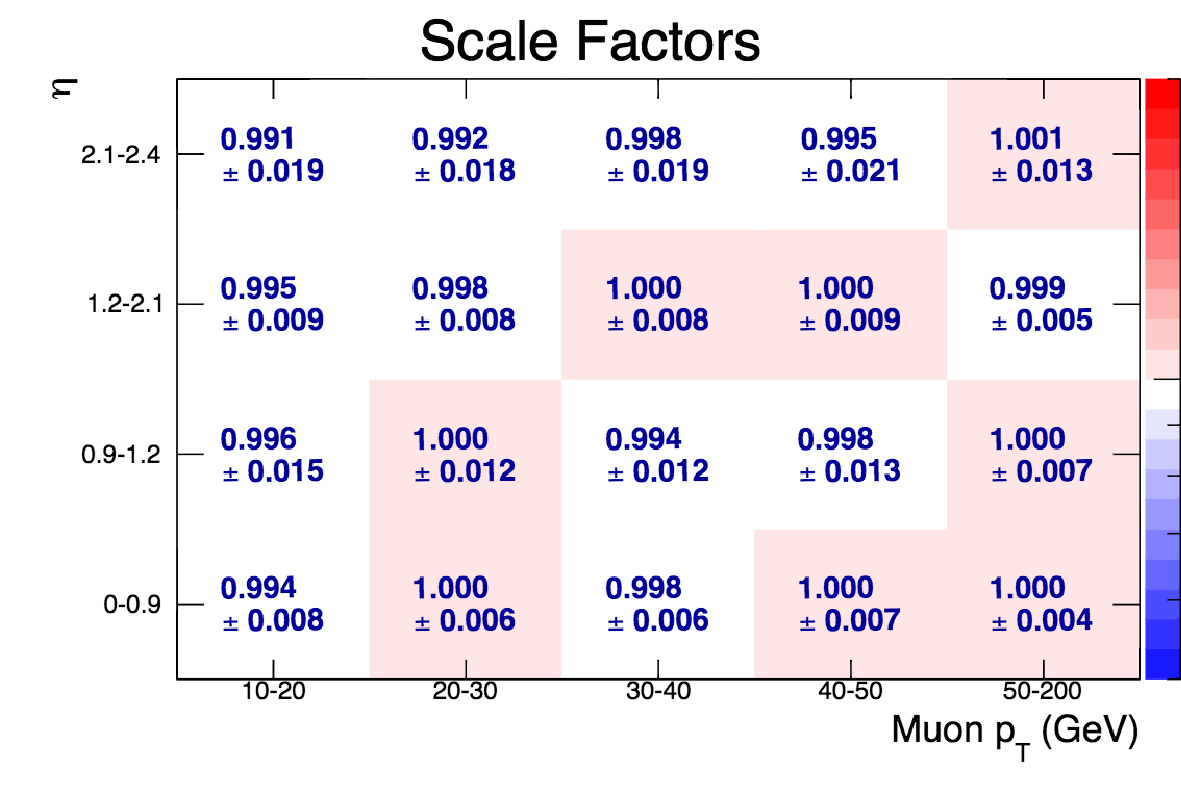
\includegraphics[width=0.4\textwidth]{evtsel/figs/sf_mu_mini02.pdf}  \\
    \end{tabular}
    \caption{
      \label{fig:sf_muons}
      Muon scale factors as a function of \pt\ and $\eta$.
      The left plot shows the scale factors associated with the ID selection criteria,
      and the right plot shows the scale factors associated with the isolation selection criteria.
      Each scale factor is applied as an event weight once per muon in the event.
    }
  \end{center}
\end{figure}

\begin{figure}[!ht]
  \begin{center}
    \begin{tabular}{cc}
      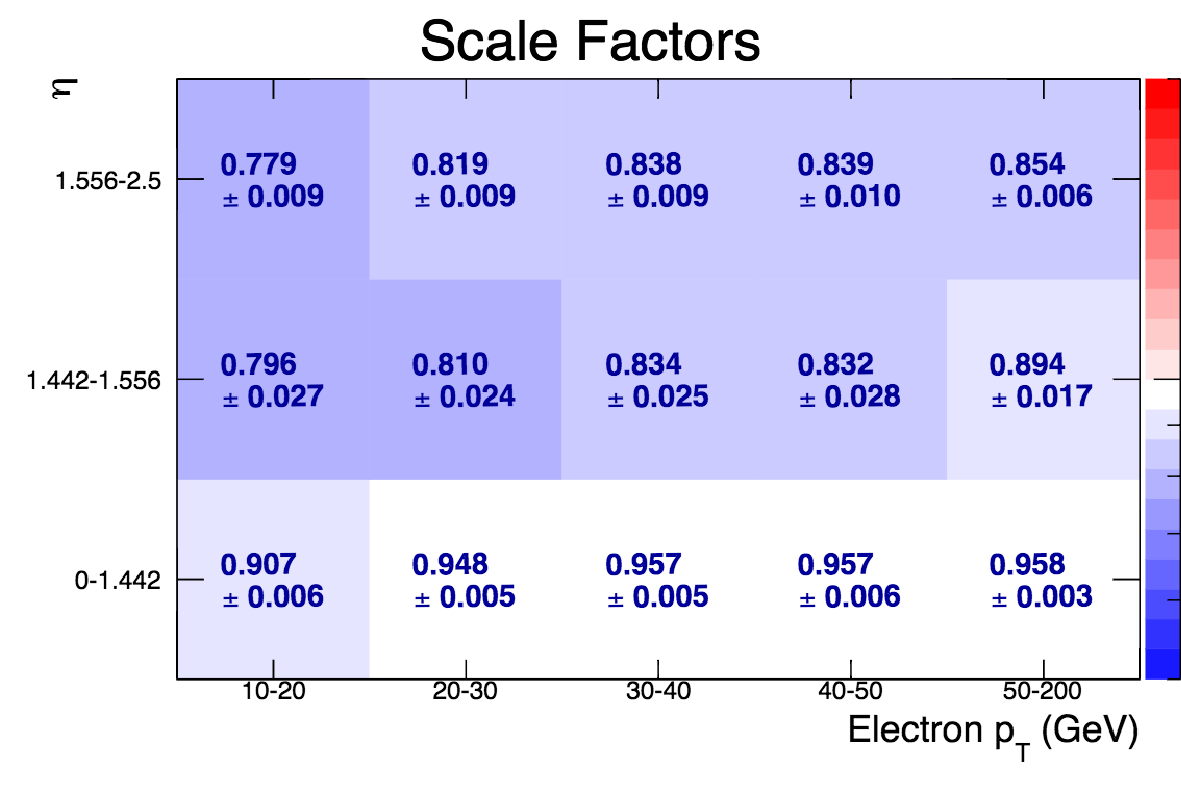
\includegraphics[width=0.4\textwidth]{evtsel/figs/FS_sf_el_tight_mini01.pdf}  &
      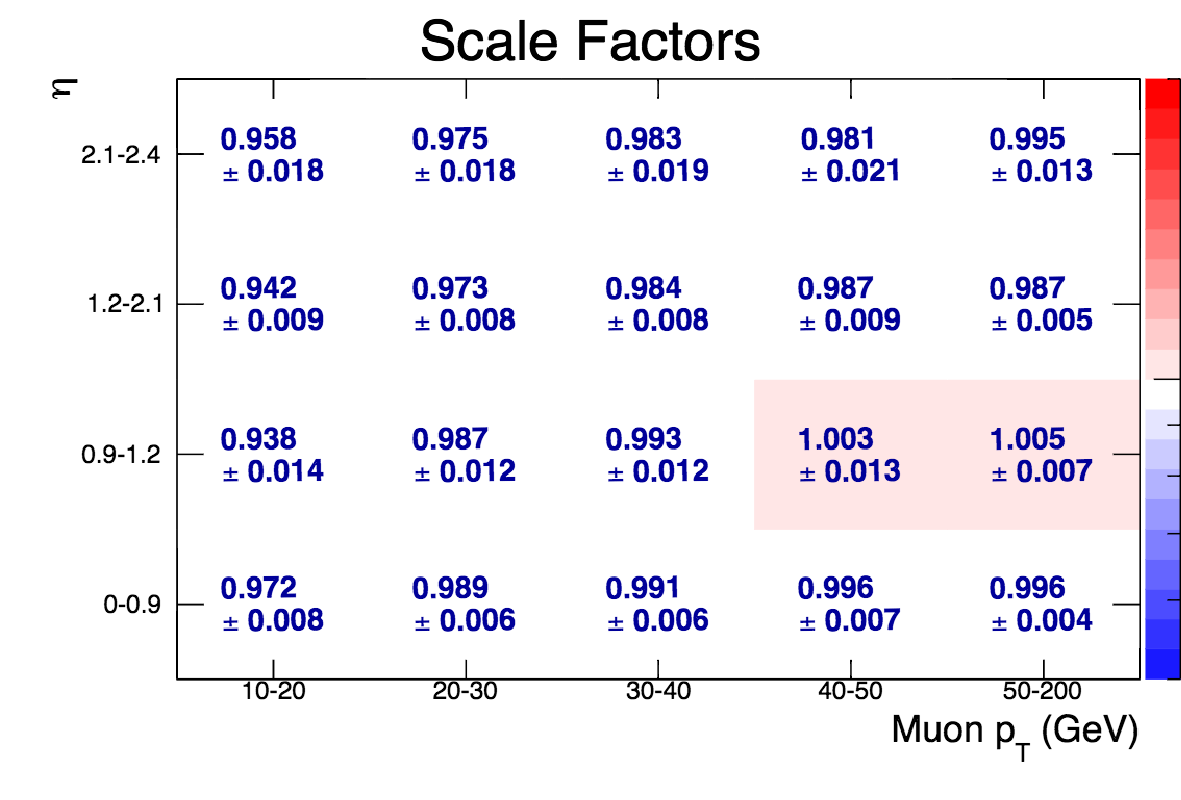
\includegraphics[width=0.4\textwidth]{evtsel/figs/FS_sf_mu_mediumID_mini02.pdf}  \\
    \end{tabular}
    \caption{
      \label{fig:FS_sfs}
      Fastsim scale factors as a function of \pt\ and $\eta$.
      The left plot shows the scale factors applied per electron,
      and the right plot shows the scale factors applied per muon.
      Each scale factor is applied as an event weight once per lepton in the event.
    }
  \end{center}
\end{figure}

\clearpage

\subsection{Electron Selection}
\label{ssec:elsel}
Output from a multivariate analysis (MVA) is used to identify the electrons used in this analysis~\cite{egamma13tev} based on a method used previously~\cite{egamma8tev}.
This is done separately in the barrel and endcap using a variety of kinematic variables as input.
Electrons with \pt $>$ 15 GeV and $|\eta|<2.4$ are considered.
The training of the MVA is done using a Z+jets MC sample where the electrons used as signal input are
required to be matched to generator level electrons, and electrons used as background are required to not be matched.

Variables used to differentiate electrons from fakes mainly use information from the tracker and ECAL.
Measurements made by the ECAL and tracker are compared using the ratio of the electron cluster energy to the track momentum at the outermost track layer.
This ratio is expected to be 1 for real electrons, but not necessarily for fakes.
$\sigma_{i\eta i\eta}$ is a purely calometric variable which uses the shower shape of the electron object to differentiate real and fake electrons.
The main premise behind this variable is that electron energies are contained within 1-2 crystals in $\eta$
where ECAL energy from jets is spread across many crystals leading to the shape for real electrons and fake electrons to be very different making it a good variable to differentiate the two.
A way to differentiate real and fake electrons is to check the consistency of the track of the reconstructed electron object left in the tracker.
This is done by measuring the difference in $\eta$ of the track measured in the outer layer and the electron cluster in the ECAL ($\mathrm{\Delta\eta(track-cluster)}$).
An plot showing how each of these variables looks for real and fake electrons is shown in figure~\ref{fig:electron_mva_vars}.

\begin{figure}[!htb]
  \begin{center}
    \begin{tabular}{cc}
      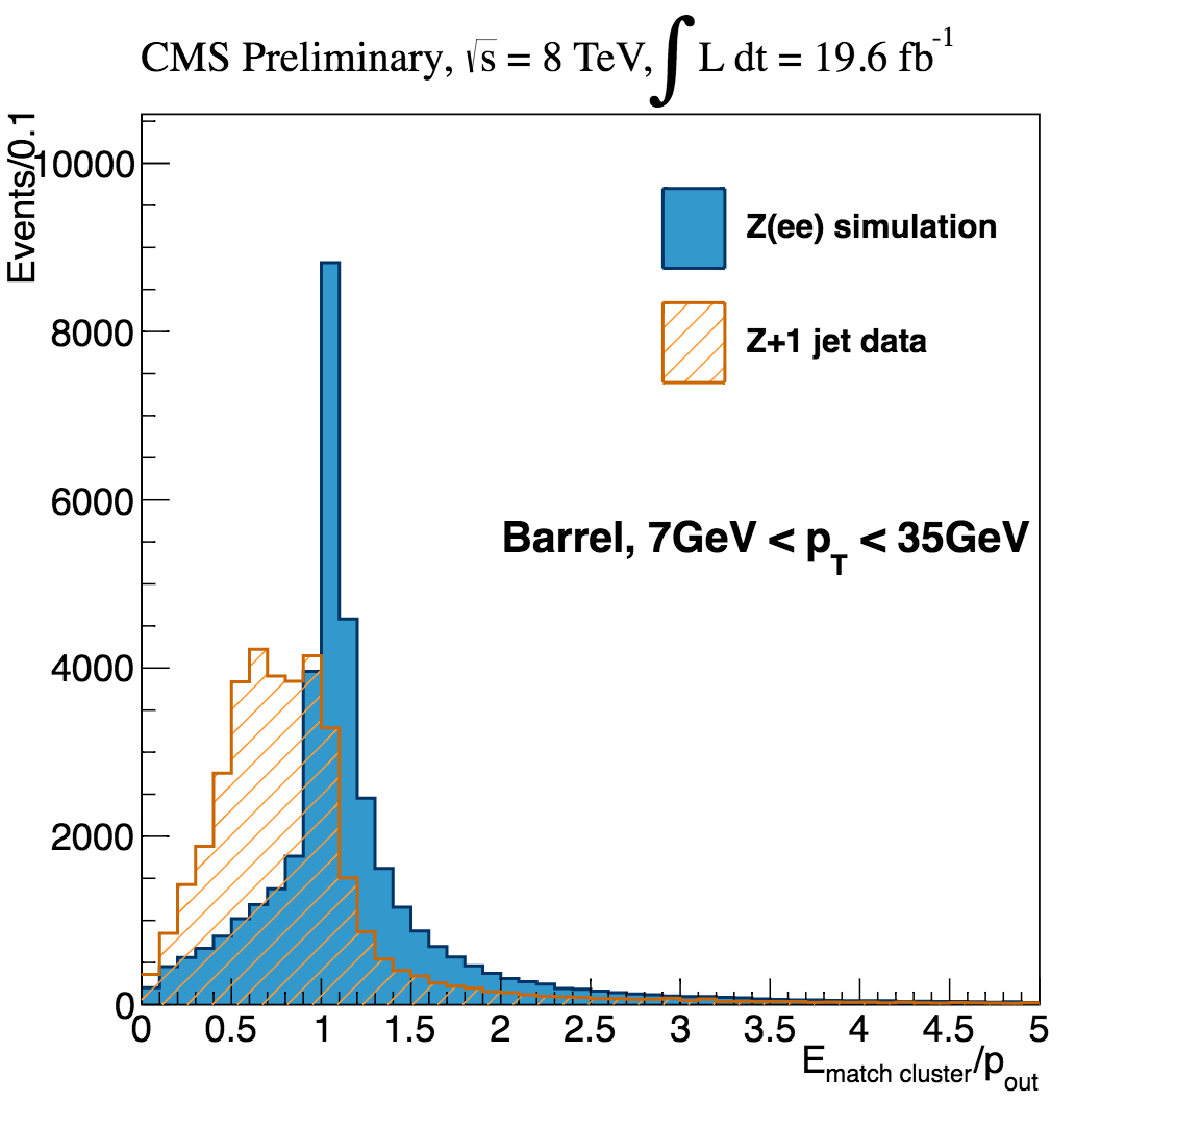
\includegraphics[width=0.4\textwidth]{evtsel/figs/EoPout_EB_LowPt.pdf} &
      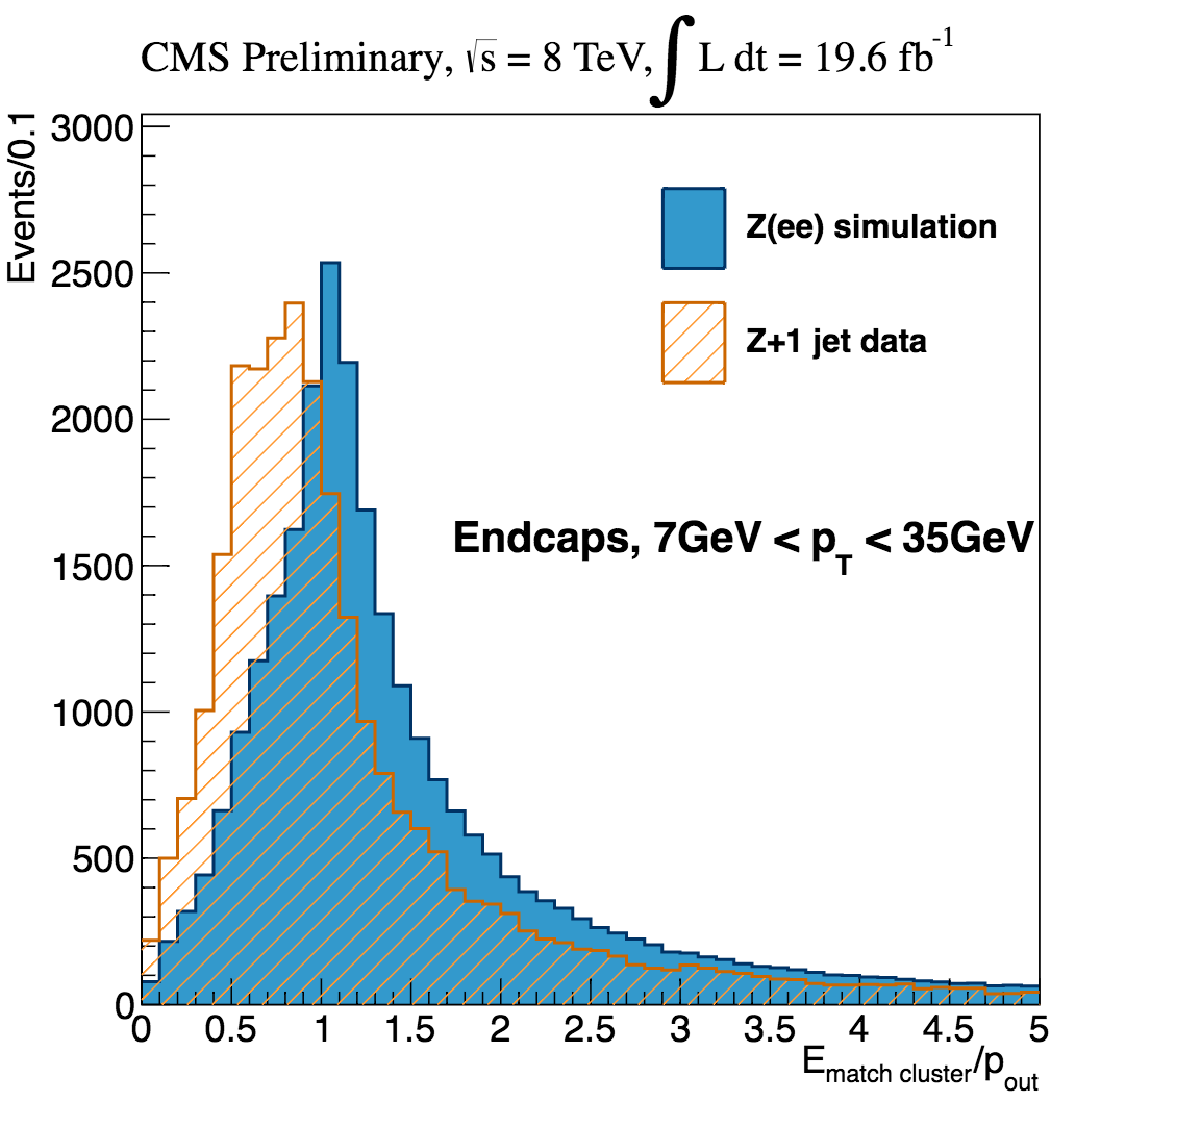
\includegraphics[width=0.4\textwidth]{evtsel/figs/EoPout_EE_LowPt.pdf} \\      
      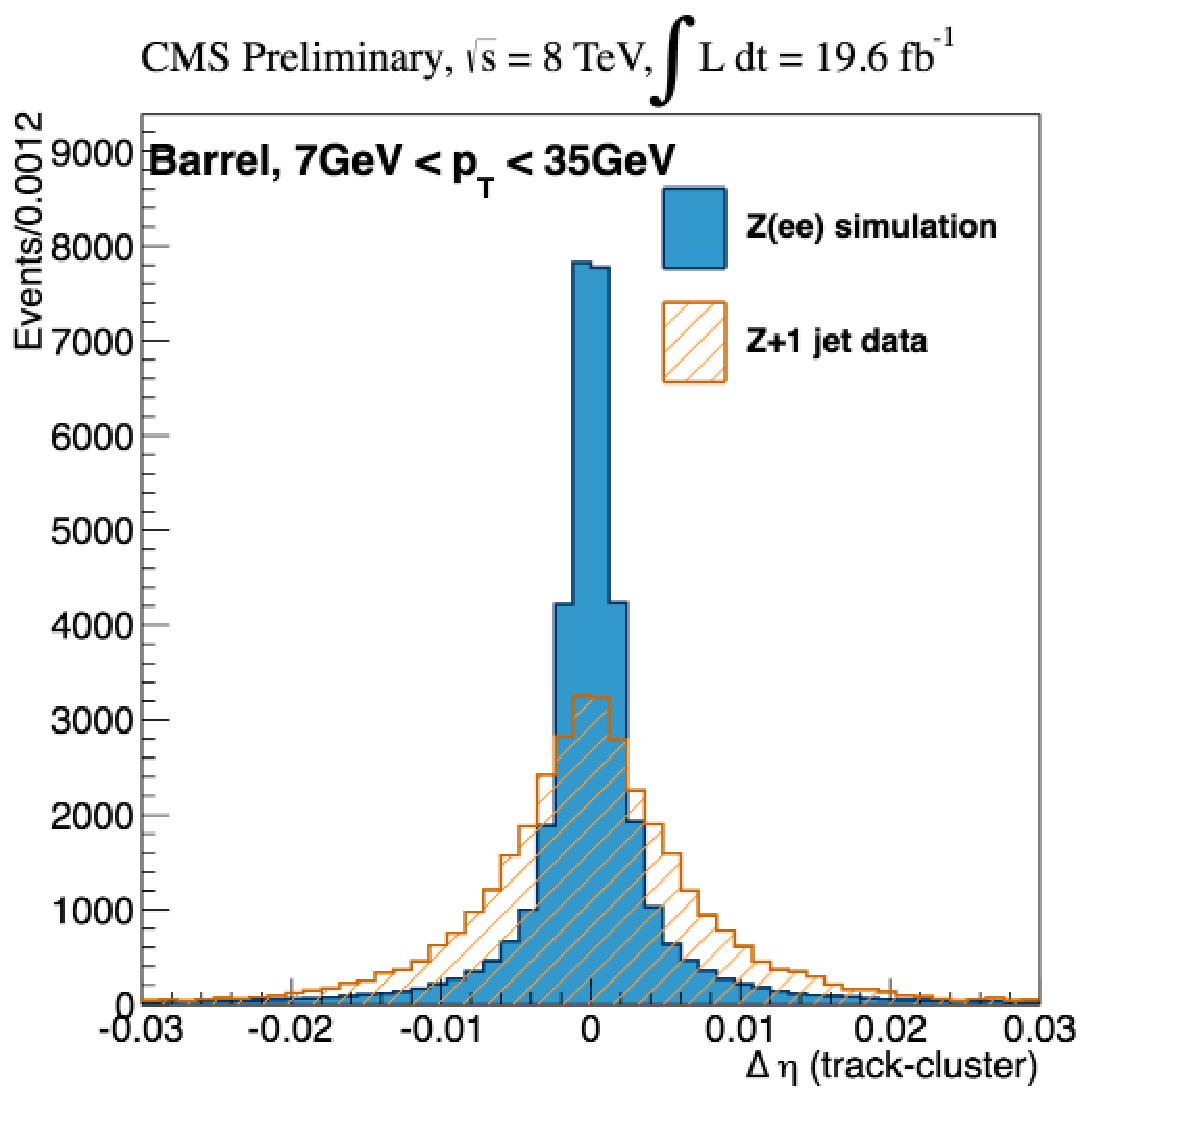
\includegraphics[width=0.4\textwidth]{evtsel/figs/deltaEta_EB_LowPt.pdf} &
      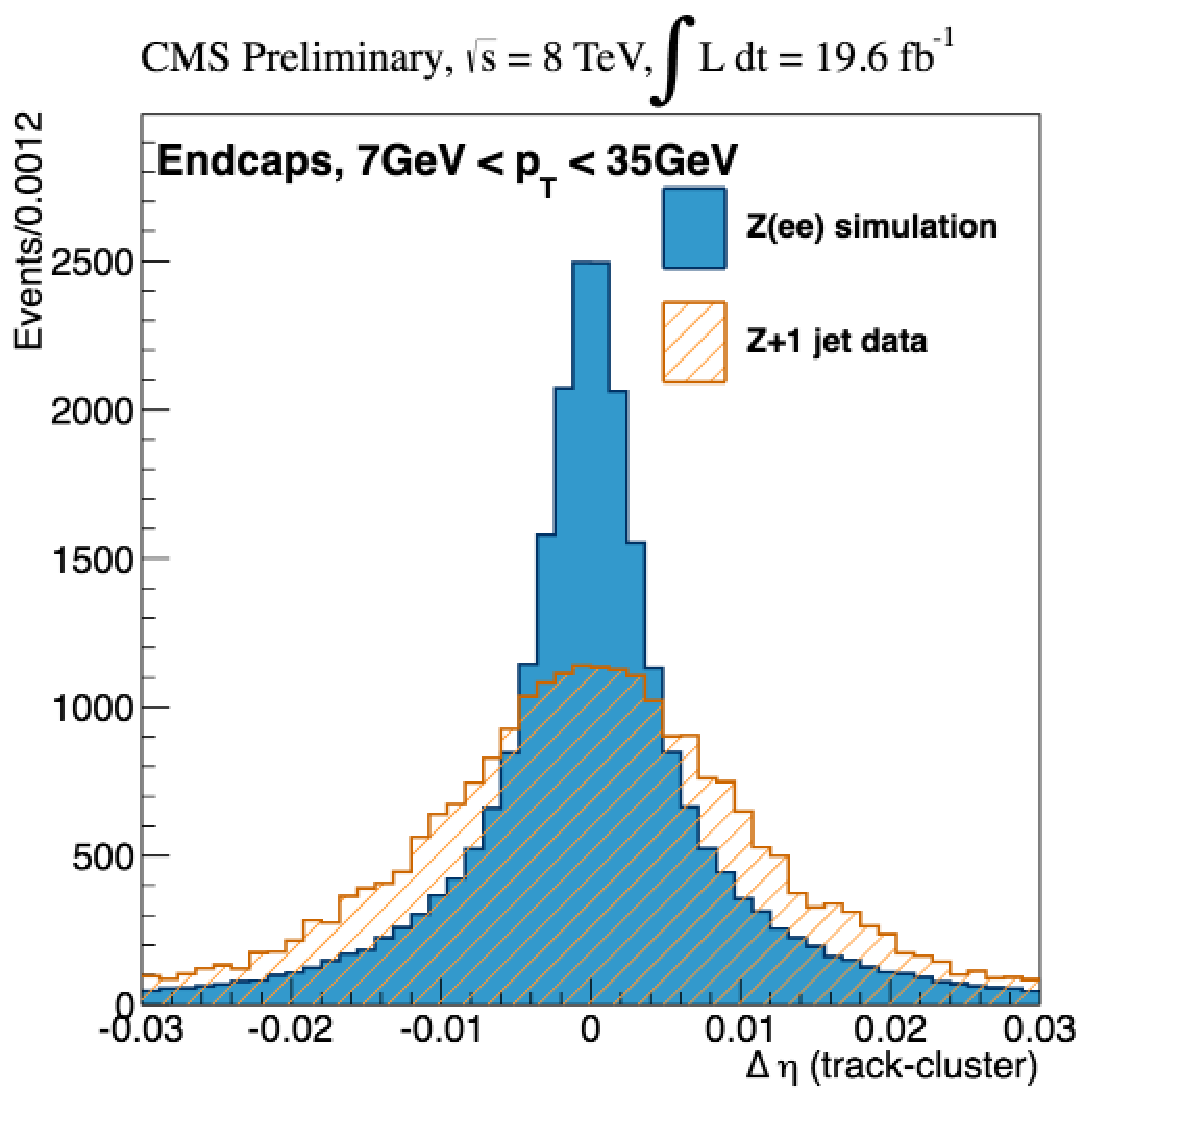
\includegraphics[width=0.4\textwidth]{evtsel/figs/deltaEta_EE_LowPt.pdf} \\      
      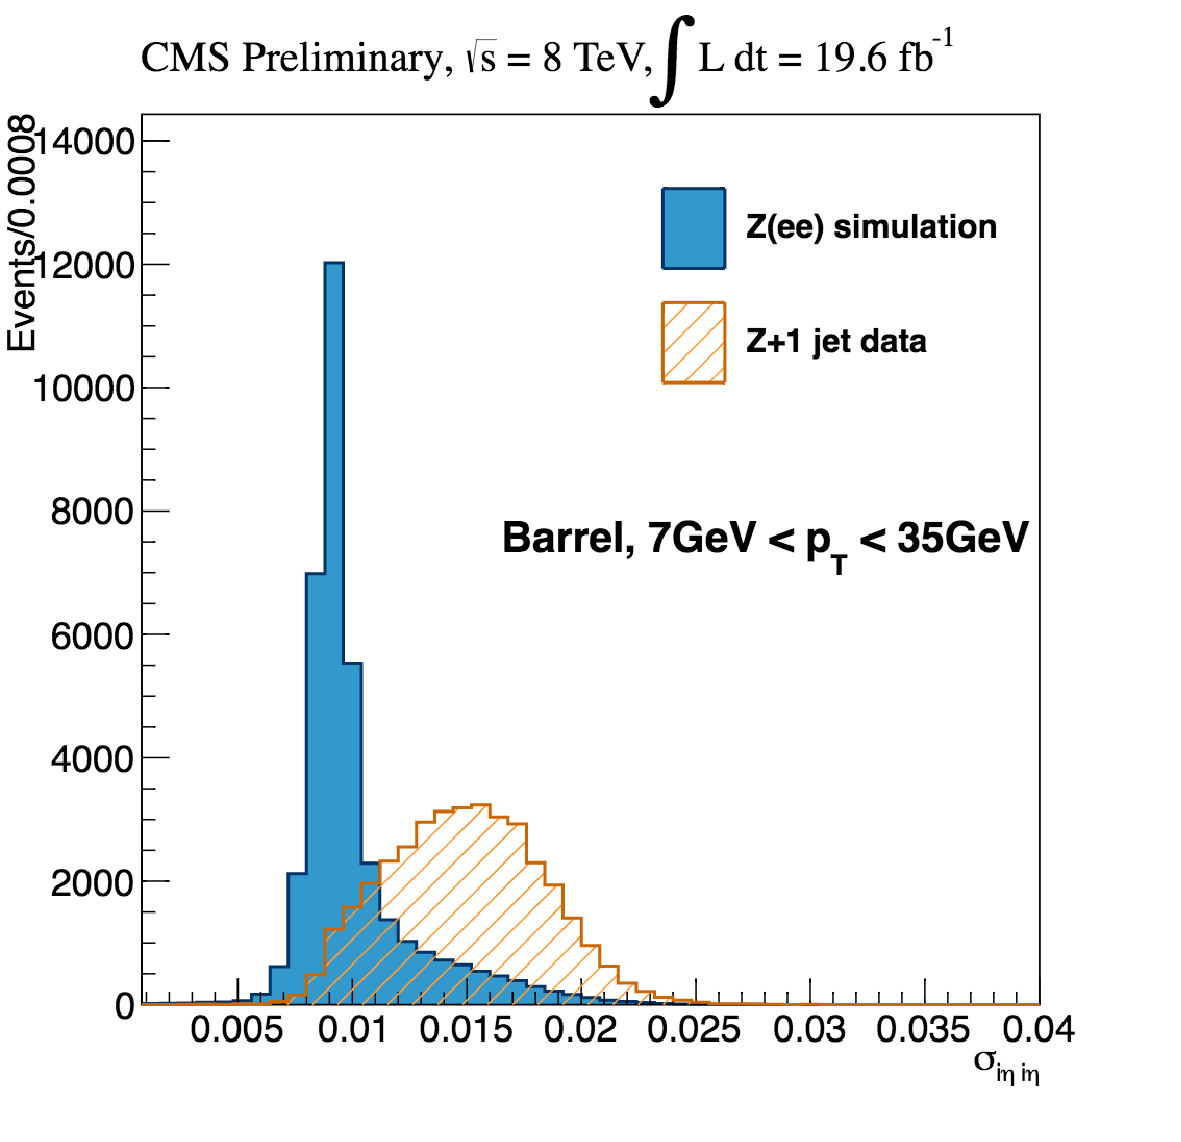
\includegraphics[width=0.4\textwidth]{evtsel/figs/see_EB_LowPt.pdf} &
      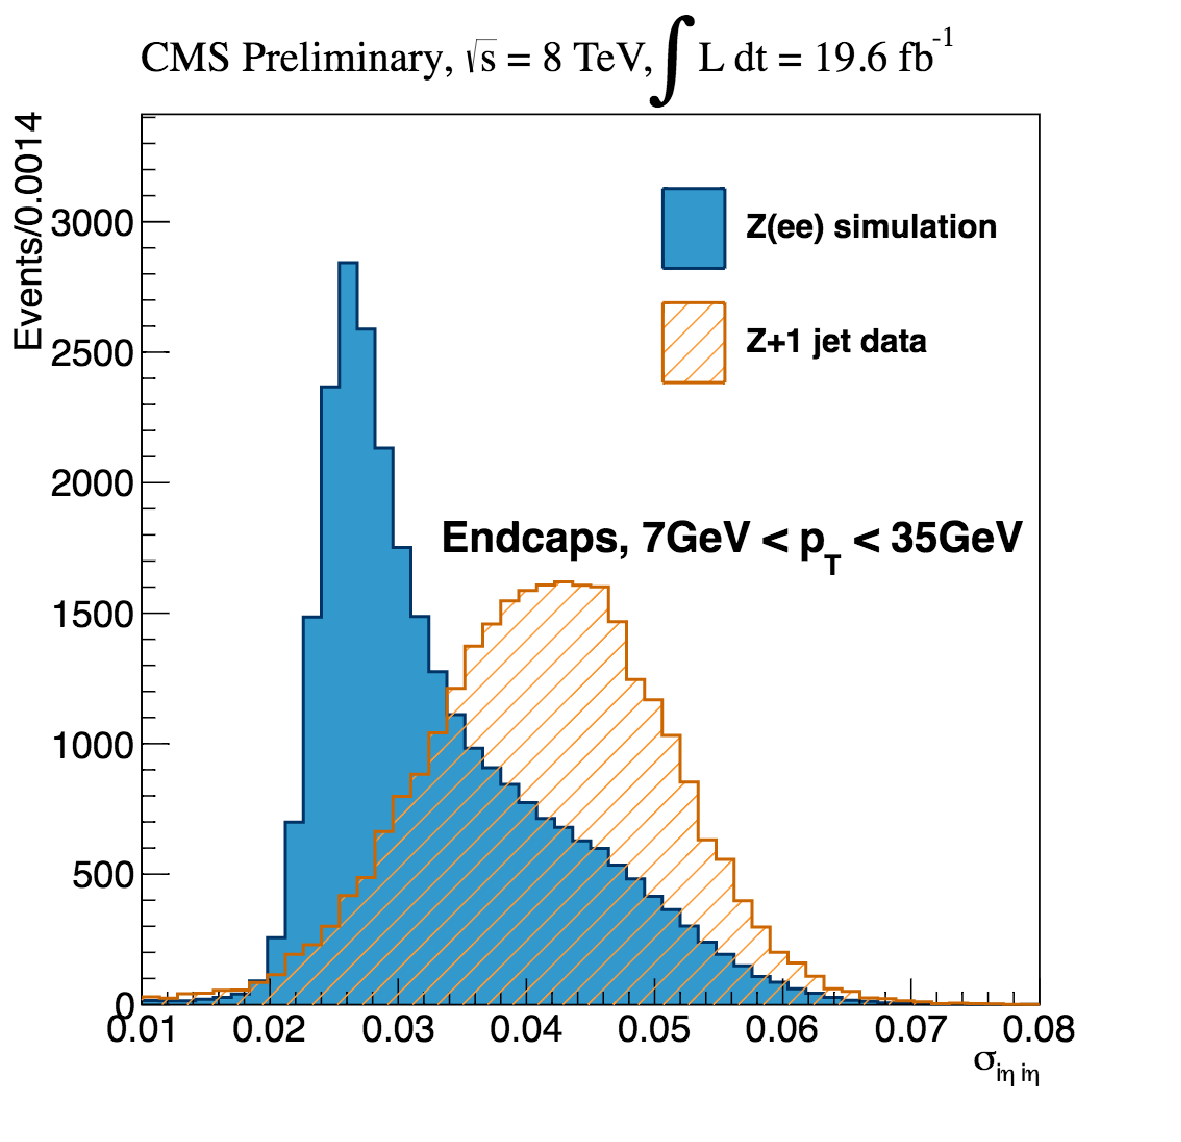
\includegraphics[width=0.4\textwidth]{evtsel/figs/see_EE_LowPt.pdf} \\      
    \end{tabular}
    \caption{
      \label{fig:electron_mva_vars}
      Kinematic variables used to distinguish real electrons from fake electrons are shown
      with electrons in the barrel on the left and electrons in the endcap on the right.
    }
  \end{center}
\end{figure}
  
Electrons in data are compared to the electrons from MC using the probe leg from a
``tag and probe'' technique similar to the one described in section~\ref{ssec:lepscalefactors}.
The requirements for the probe electron are as follows:
\begin{itemize}
\item $\mathrm{p_{T}(e) > 10~GeV}$
\item $\mathrm{\eta(e) < 2.5}$
\item Loose identification criteria
\item Relative isolation (pileup corrected) < 0.1
\end{itemize}
The output of this MVA is shown in figure~\ref{fig:electron_mva},
and the MVA cut requirement for this analysis is shown in table~\ref{table:electrons}.
  
\begin{figure}[!ht]
  \begin{center}
      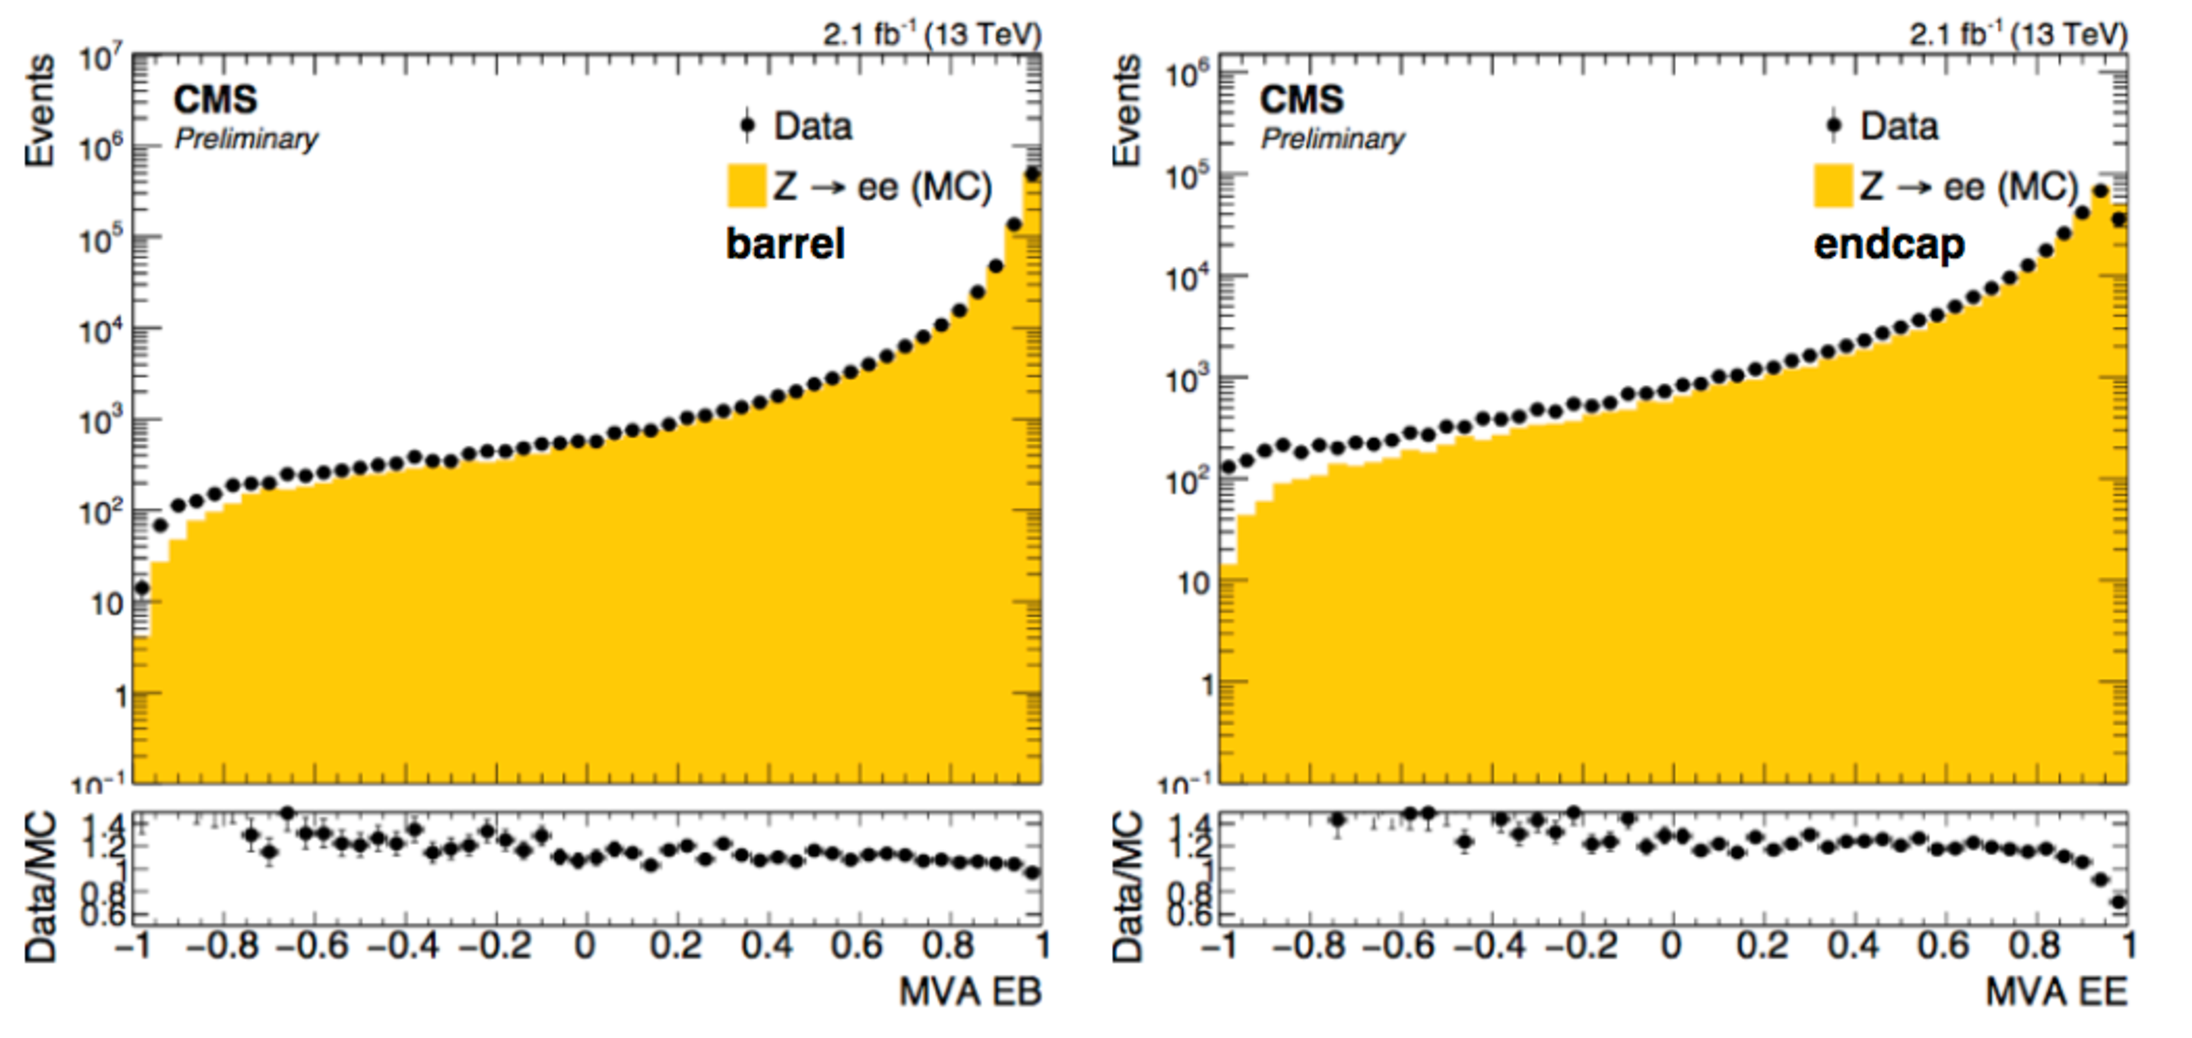
\includegraphics[width=0.8\textwidth]{evtsel/figs/Electron_MVA_2015.pdf}
    \caption{
      \label{fig:electron_mva}
      Output of the electron MVA is shown comparing electrons in data vs. MC with electrons in the barrel on the left and the endcap on the right.
      The electrons shown are the probe leg when using a ``Tag and Probe'' technique.
    }
  \end{center}
\end{figure}
  
\begin{table}[!htb]
  \begin{center}
    \caption{
      \label{table:electrons}
      Requirements for electrons with \pt\ $>$ 10 \gev.
    }
    \begin{tabular}{l|cc}
      \hline
      Region                & MVA minimum cut value \\
      \hline
      Barrel $|\eta| < 0.8$ & 0.913286 \\
      Barrel $|\eta| > 0.8$ & 0.805013 \\
      Endcap                & 0.358969 \\
      \hline
      \hline
      Cut variable                  & Requirement   \\
      \hline
      $d_{0}$ (w.r.t. 1st good PV)   & $<0.05$ cm  \\
      $d_{z}$ (w.r.t. 1st good PV)   & $<0.1$  cm  \\
      miniRelIso / \pt              &  $<0.10$ \\
      \hline
    \end{tabular}
  \end{center}
\end{table}

The efficiency of the electron selection is measured to be on average 80\% for electrons with $\mathrm{p_{T} >~ 20~GeV}$ as seen in figure~\ref{fig:electronideff}.

\begin{figure}[!ht]
  \begin{center}
      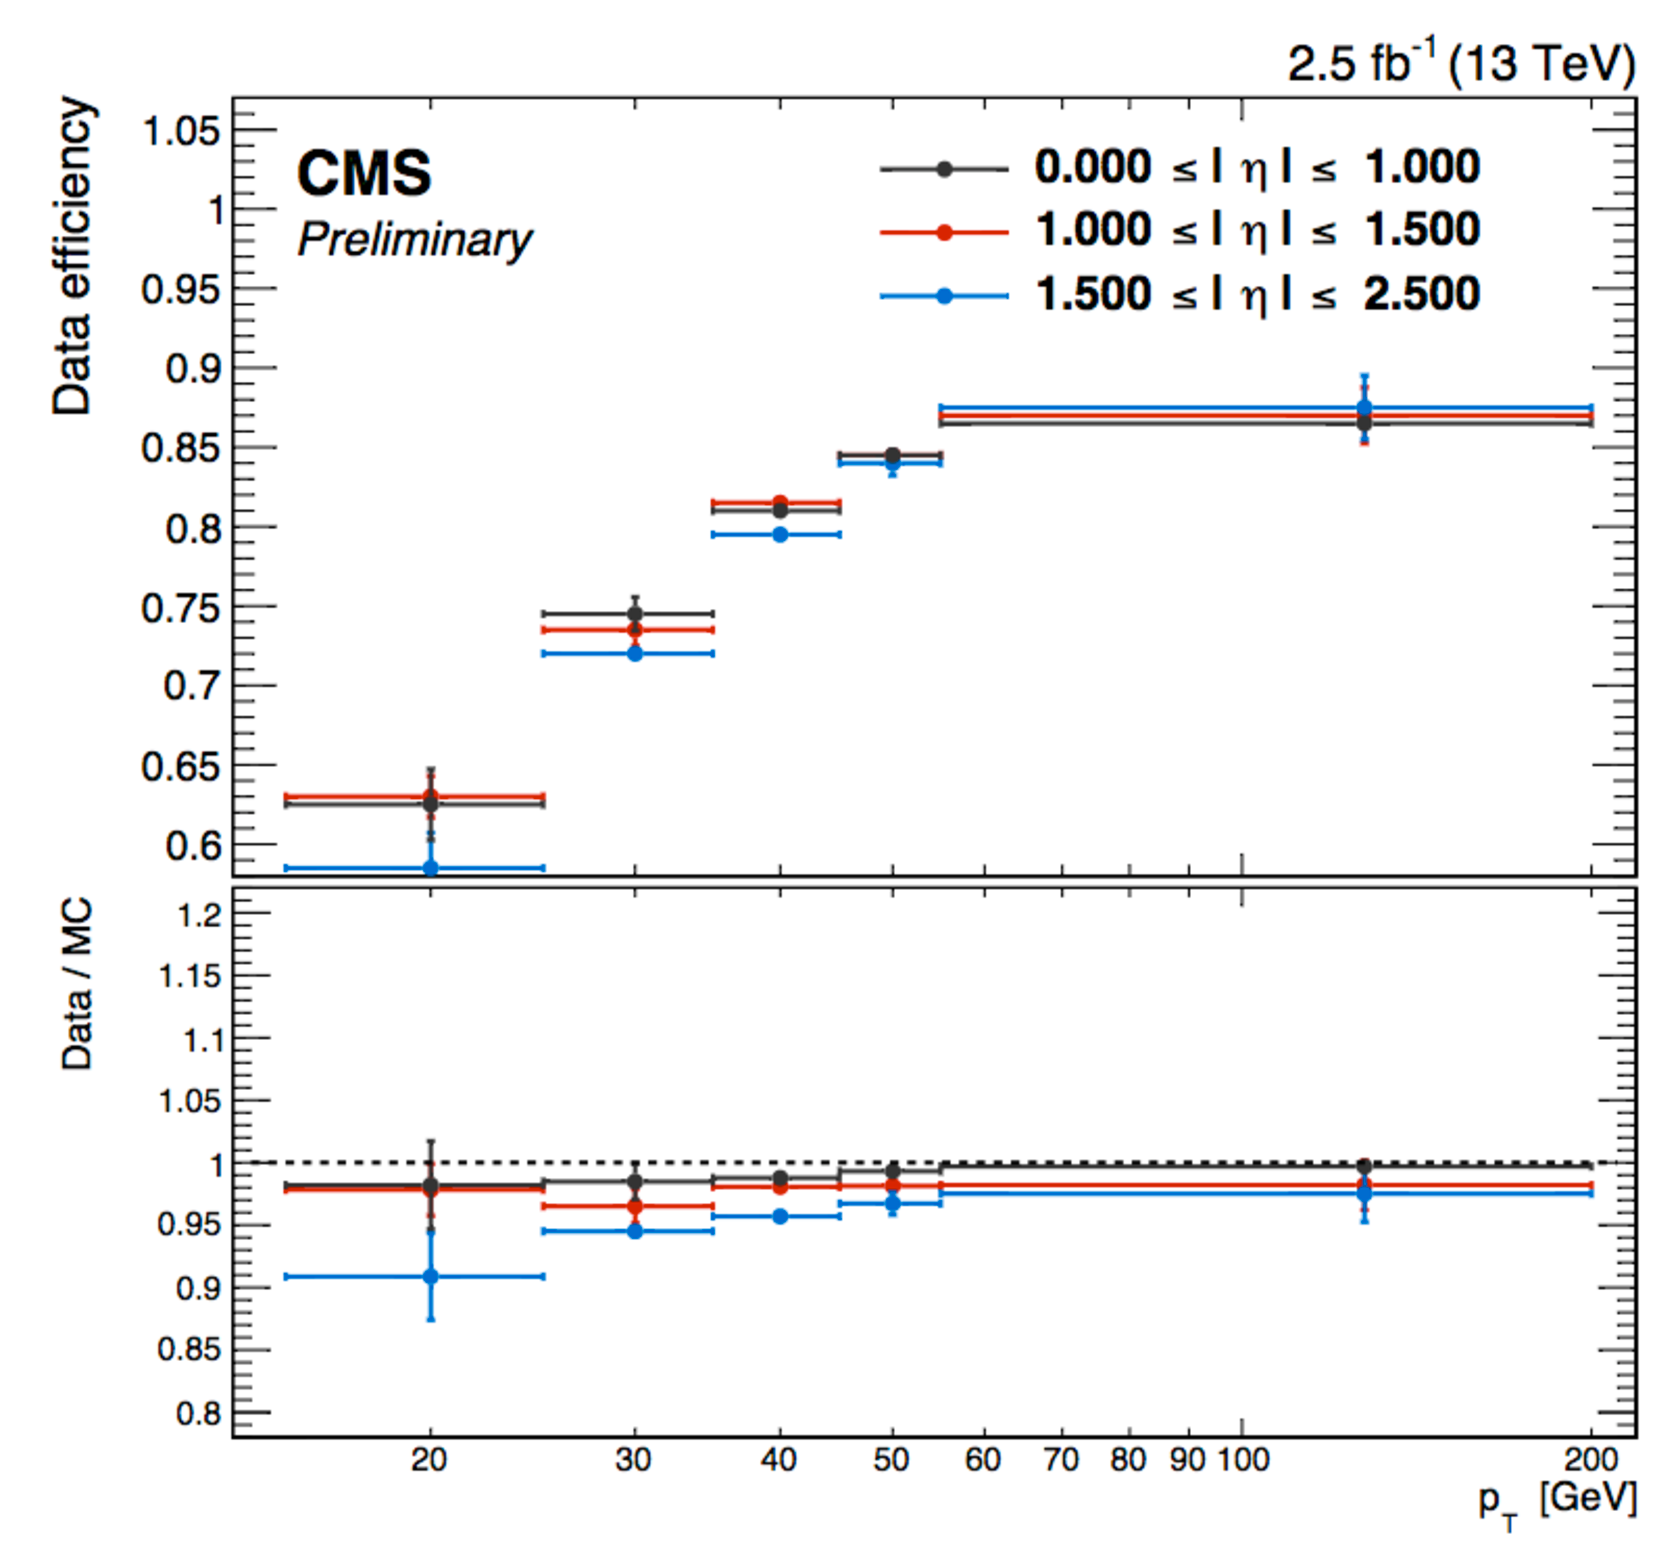
\includegraphics[width=0.8\textwidth]{evtsel/figs/Electron_MVA_efficiency.pdf}
    \caption{
      \label{fig:electronideff}
      Electron identification efficiency in data (top) and data to MC efficiency ratios (bottom)
      measured for the identification criteria based on a MVA discriminant with an average efficiency of 80\%.
      The efficiency is measured with the tag and probe method and shown in three pseudorapidity ranges as a function of the electron transverse momentum.
    }
  \end{center}
\end{figure}
  

\subsection{Muon Selection}
\label{ssec:musel}
The muon selection criteria is based on studies performed by the muon POG at CMS~\cite{tdr1}\cite{muonReco}.
Muons with \pt $>$ 15 GeV and $|\eta|<2.4$ are considered. 
The baseline muon selection requires that the muon be identified as a muon by the particle flow algorithm,
as well as being identified as a tracker or global muon.
To define a tracker muon, all tracks in the tracker with \pt $>$~0.5 \gev\ and $p~>~2.5$~\gev are considered.
These tracks are extrapolated to the muon system and then required to to have a matching hit in at least one muon segment.
Global muons are defined by matching a tracker track with that of a track reconstructed independently by the muon system.
After the two tracks are matched, a global muon track fit is done combining the hits from the two separate tracks.
Muons in this analysis must either qualify as a global muon or pass a segment compatibility requirement.
Segment compatibility is defined using a template based on simulation.
In addition to these requirements, muons are required to be within 0.05 cm of the primary vertex in the x-y direction and within 0.1 cm in the z direction.
The full muon selection requirements are listed in Table~\ref{tab:muons}.

\begin{table}[htb]
\begin{center}
\caption{\label{tab:muons} Summary of the muons selection requirements.}
\begin{tabular}{l|c}
\hline
\hline
good Global Muon Requirements & \\
\hline
              Quantity   &     Requirement \\
\hline
Fraction of valid tracker hits    & $>$ 0.8   \\ 
Normalized global-track $\chi^2$  & $<$ 3     \\
Tracker-Standalone position match & $<$ 12    \\
Kick finder                       & $<$ 20    \\
Segment compatibility             & $>$ 0.303 \\
\hline
tight segment compatibility & $>$ 0.451 or passes above requirements \\
\hline
\hline
muon type & (global or tracker) and PF muon \\
\hline
$d_{0}$ (w.r.t. 1st good PV)       & $<0.05$ cm  \\
$d_{z}$ (w.r.t. 1st good PV)       & $<0.1$ cm   \\
miniRelIso / \pt                  & $<0.20$ \\
\hline
\end{tabular}
\end{center}
\end{table}


\subsection{Photons}
\label{ssec:phosel}
In this analysis it is not necessary that the photon sample is high in purity,
it is only required that the photon-like object in each event is well-measured.
The reason for this is discussed in more detail in section~\ref{sec:bkg_zjets}.
Photons are required to pass a loose working point designed by the EGamma POG at CMS with some additional cuts.
This working point was designed to be 90\% efficient with a background rejection of greater than 80\%,
and photons with \pt $>$ 22 \gev\ and $\eta~<$~2.4 are considered.
Photons that are in the transition region between the ECAL barrel and ECAL endcap are vetoed,
specifically photons with 1.4$~<~\eta~<$~1.6.
Cuts made on different versions of the photon object's isolation calculated using independent sets of reconstructed particle flow objects.
A cut is made on absolute pf charged hadron isolation with no corrections,
and then cuts are made to the neutral hadron and photon isolations after applying $\rho$~corrections as described in section~\ref{ssec:isolation}.
Due to the different response of the detector in the barrel and endcap, the cuts are tuned separately for these regions.
The cuts on neutral isolation are made as a function of the photon \pt, and all the isolation requirements are listed in table~\ref{tab:photons}.


\begin{table}[htb]
  \begin{center}
    \caption{
      \label{tab:photons}
      Summary of the photon isolation requirements.
    }
    \begin{tabular}{l|l|l}
      \hline
      \hline
      PF objects                      &Requirement in barrel                    &Requirement in endcap \\
      \hline
      charged hadron                  &$<$~3.32                                 &$<$~1.97                                    \\
      $\rho$ corrected neutral hadron &$<$~1.92 + 0.014*$\mathrm{p_{T}(\gamma)}$ &$<$~11.86 + 0.0139*$\mathrm{p_{T}(\gamma)}$ \\
                                      &+0.000019*$\mathrm{p_{T}^{2}(\gamma)}$     &+0.000025*$\mathrm{p_{T}^{2}(\gamma)}$       \\
      $\rho$ corrected photon         &$<$~0.81 + 0.0053*$\mathrm{p_{T}(\gamma)}$&$<$~0.83 + 0.0034*$\mathrm{p_{T}(\gamma)}$  \\
      \hline
      \hline      
    \end{tabular}
  \end{center}
\end{table}

In addition to the isolation requirements, further cuts are made on photons to maximize the energy resolution of the photon and also remove events with real \MET.
The photon is required to be mostly electromagnetic, and a cut is made on the ratio of hadronic energy to electromagnetic energy ($\mathrm{\frac{H}{E}}$).
In order to reject fake photons from $\pi^{0}$ decays, a requirement is made of $\mathrm{\sigma_{i\eta i\eta}~<~}$0.0102 (0.274) for photons in the barrel (endcap).
It is possible to end up with real \MET in photon events in the process of W$\rightarrow e+\mathrm{\bar{\nu_{e}}}$
where the electron immediately radiates most of its energy away in the form of a photon.
Before radiating away its energy, it is possible for the electron to leave a track in the pixel layer,
therefore in order to remove these events, it is required that there be no pixel track matched to the photon.
These events are also removed by rejecting photons which have an electron of at least \pt $>$ 10 GeV matched within a cone of $\mathrm{dR} < 0.2$.
It is required that a pfjet with \pt\ $>~$10 \gev\ be matched to the photon with a cone of $\Delta R~<~0.3$. 
The matched jet is then required to have an overall electromagnetic energy fraction of at least 70\%.
Lastly, events with a photon that is aligned with \MET\ having $\Delta\phi~<~0.14$ are removed. 
The full photon requirement is listed in~\ref{tab:photonselection}.

\begin{table}[htb]
  \begin{center}
    \caption{
      \label{tab:photonselection}
      Summary of the photon selection requirements.
    }
    \begin{tabular}[width=0.4\textwidth]{l|l}
      \hline
      \hline
      Quantity & Requirement \\
      \hline
      \pt                                            &$>~$22 \gev  \\
      $|\eta|$                                       &$~<~$2.4     \\
      veto photons in transition region              &$|\eta|$:1.4 -- 1.6      \\
      $\mathrm{\frac{H}{E}}$                         &$~<~$0.5     \\
      $\mathrm{\sigma_{i\eta i\eta}}$ (barrel)          &$~<~$0.0102  \\
      $\mathrm{\sigma_{i\eta i\eta}}$ (endcap)          &$~<~$0.274   \\
      $\mathrm{\Delta\phi(\gamma,E_{T}^{miss})}$       &$~>~$0.14    \\
      \hline
    %% \end{tabular}
    %% \begin{tabular}[width=0.4\textwidth]{l}
      No matching pixel track (pixel veto)                       & \\
      reject $\gamma$ within $dR<0.2$ of an electron             & \\
      Matched to a pfjet with emfrac$~>~$0.7                     & \\
      \hline
      \hline      
    \end{tabular}
  \end{center}
\end{table}

\subsection{MET}
\label{ssec:MET}
Type 1 corrected \MET\ is used in this analysis, and a full description can be found in chapter~\ref{ch:MET}.

\subsection{\texorpdfstring{$\mathrm{H_{T}}$}{HT}}
\label{ssec:HT}

The signal model targeted by this analysis is expected to have large amounts of hadronic activity.
A simple way to quantify the amount of hadronic activity in an event is to use the variable ``$H_{T}$''.
\HT\ can be simply described as the scalar sum of the \pt\ of the jets in the event and is defined by the equation~\ref{eqn:HT}.

\begin{equation}
  \label{eqn:HT}
  H_{T} = \sum{\mathrm{|\mathbf{p}_{T}(jet)|}}
\end{equation}

\subsection{Jets}
\label{ssec:jetsel}

The jets used in this analysis are described in section~\ref{ssec:jets}.
Jets with \pt\ $>$ 35 \gev and  $|\eta| < 2.4$~are used
with the L1, L2 and L3 corrections applied to MC and the additional ResidualL2L3 corrections applied to data.
The residualL2L3 correction is used to correct the scale of the jets in MC to match what is measured in data as a function of the jet's \pt, and $\eta$.
A loose selection criteria, listed in table~\ref{tab:jetlooseid}, is applied to each jet to remove jets coming from noise in the detector.
In addition to this, any jet that is found to be near a lepton within a cone of dR = 0.4 is removed from the event.
This is done to avoid possibly double counting energy.
The full jet selection is listed in table~\ref{tab:jetsel}.

\begin{table}[htb]
  \begin{center}
    \caption{
      \label{tab:jetlooseid}
      Criteria for a jet to pass the loose ID requirement.
    }
    \begin{tabular}[width=0.4\textwidth]{l|l}
      \hline
      \hline
      Quantity & Requirement \\
      \hline
      Neutral hadron fraction &$~<~$0.99 \\
      Neutral EM fraction     &$~<~$0.99 \\
      Charged hadron fraction &$~>~$0    \\
      Charged multiplicity    &$~>~$0    \\
      Charged EM fraction     &$~<~$.99  \\
      Number of constituents  &$~>~$1    \\
      \hline
      \hline      
    \end{tabular}
  \end{center}
\end{table}

\begin{table}[htb]
  \begin{center}
    \caption{
      \label{tab:jetsel}
      Summary of the jet selection requirements.
    }
    \begin{tabular}[width=0.4\textwidth]{l|l}
      \hline
      \hline
      Quantity & Requirement \\
      \hline
      \pt               &$~>~$35 \gev \\
      $|\eta|$          &$~<~$2.4     \\
      Pass loose jet ID &See table~\ref{tab:jetlooseid}      \\
      \hline
      \hline      
    \end{tabular}
  \end{center}
\end{table}

%% https://twiki.cern.ch/twiki/bin/view/CMSPublic/BTV13TeV25ns2015Jamboree
%% https://indico.cern.ch/event/323701/session/2/contribution/7/attachments/626645/862287/Hbb_140627_BTVPlansRunII_v2.pdf
In addition to using the above requirements to classify jets, it is also useful to separate jets into two categories, light-flavored and b-tagged.
This disctinction is useful since b-tagged jets tend to come from processes having top quarks in the decay chain,
and these backgrounds can be reduced by removing events with b-tagged jets.
In order for the search to remain inclusive, signal regions containing b-tagged jets are analyzed separately.

The Combined Secondary Vertex (CSV) algorithm~\cite{btagging}\cite{btagging2015} is used to tag b-jets.
This algorithm makes use of the fact that b-quarks have a larger average lifetime than lighter partons
leading to the possibility to identify a second vertex away from the primary vertex where the tracks in the b-jet are associated with this secondary vertex.
A diagram showing this process is shown in figure~\ref{fig:secondaryVTX}.
Other variables that are used to discriminate heavy flavor jets from light are the track multiplicity, jet mass and jet energy.
These variables can be seen in figures~\ref{fig:3dip},~\ref{fig:3dflightdistance}, and~\ref{fig:svmass}.
In this analysis, a working point was chosen which corresponds to the misidentification rate for b-jets to be 1\%.
For this working point, the b-tagging efficiency is measured to be 65\% per b-tag for the working point used. 
The b-tag discriminator distribution can be seen in figure~\ref{fig:csv},
and the cut value corresponding to the working point in this analysis is CSV$~>~$0.890.

\begin{figure}[!ht]
  \begin{center}
      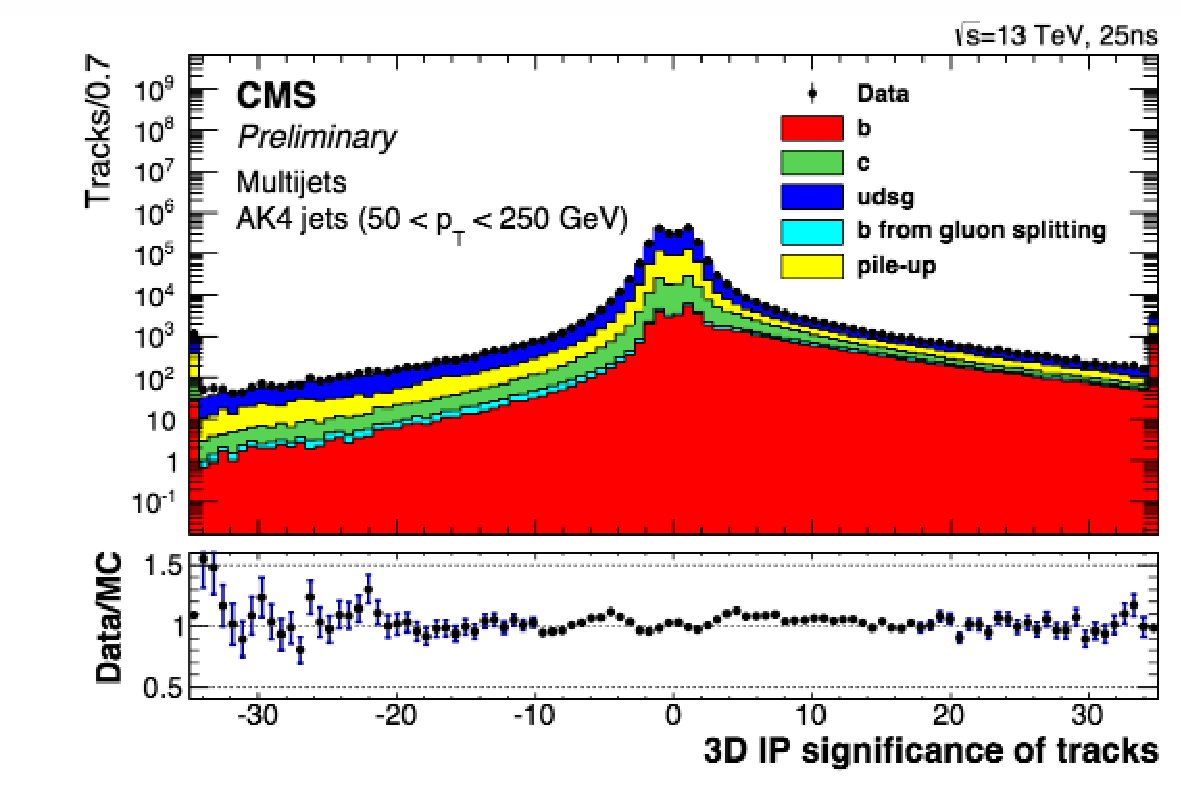
\includegraphics[width=0.8\textwidth]{evtsel/figs/CMS-PAS-BTV-15-001_Figure_001-a.pdf}
    \caption{
      \label{fig:3dip}
      A plot of the impact parameter for the secondary vertex with respect to the primary vertex
      which is used in order to differentiate jets from heavy and light flavor decay.
    }
  \end{center}
\end{figure}

\begin{figure}[!ht]
  \begin{center}
      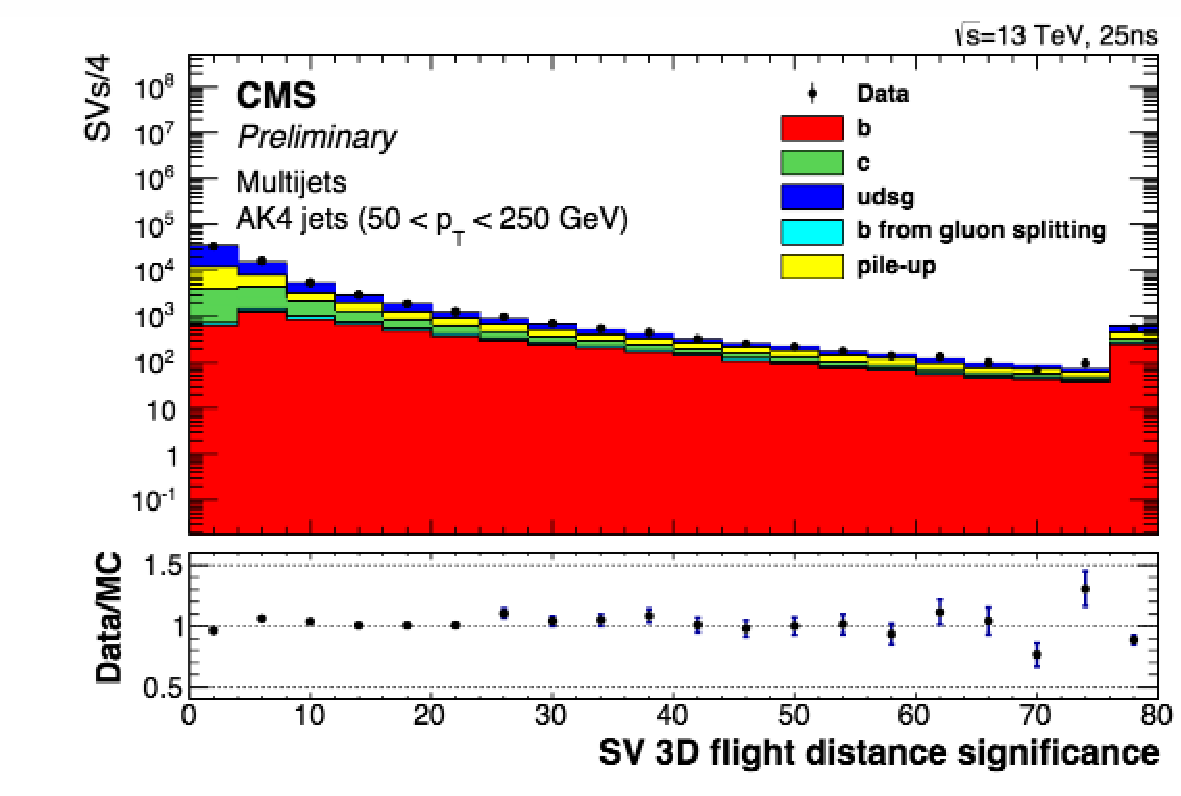
\includegraphics[width=0.8\textwidth]{evtsel/figs/CMS-PAS-BTV-15-001_Figure_002-a.pdf}
    \caption{
      \label{fig:3dflightdistance}
      A plot of the 3-D flight distance of the secondary vertex with respect to the primary vertex
      which is used in order to differentiate jets from heavy and light flavor decay.
    }
  \end{center}
\end{figure}

\begin{figure}[!ht]
  \begin{center}
      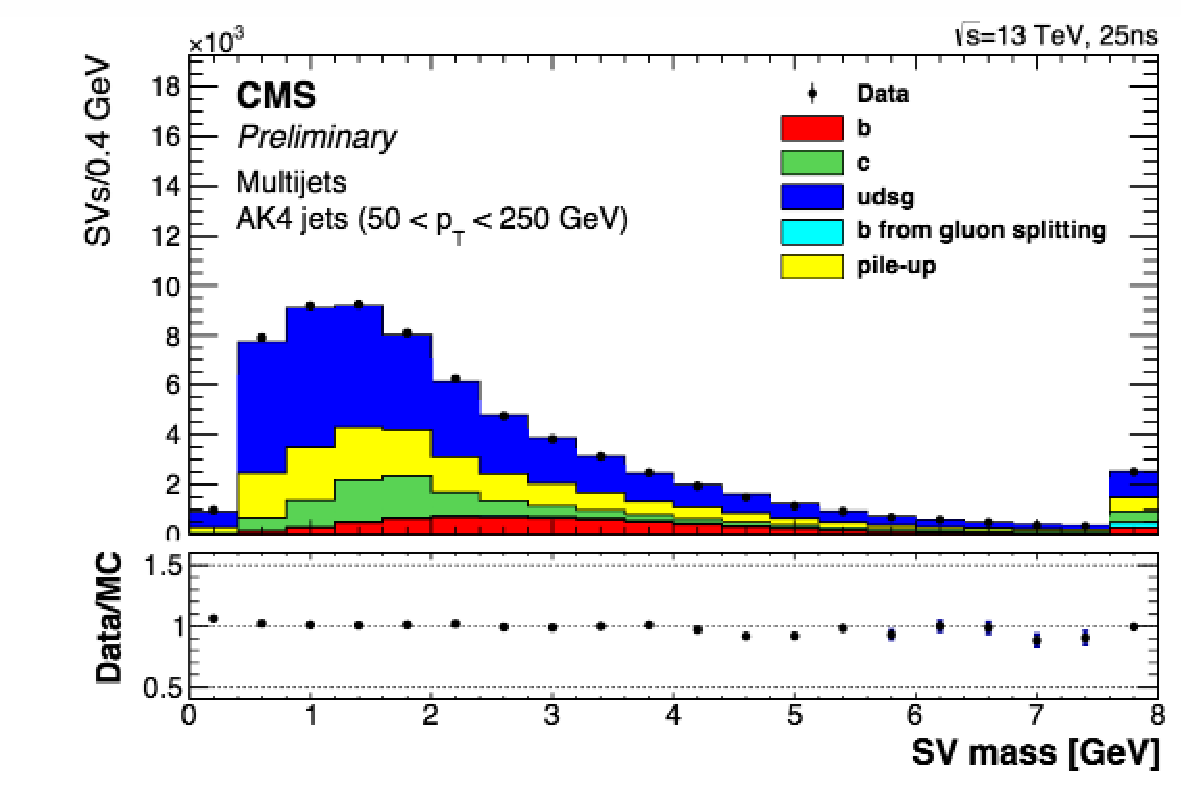
\includegraphics[width=0.8\textwidth]{evtsel/figs/CMS-PAS-BTV-15-001_Figure_002-d.pdf}
    \caption{
      \label{fig:svmass}
      A plot of the mass of the jet originating at the secondary vertex
      which is used in order to differentiate jets from heavy and light flavor decay.
    }
  \end{center}
\end{figure}

\begin{figure}[!ht]
  \begin{center}
      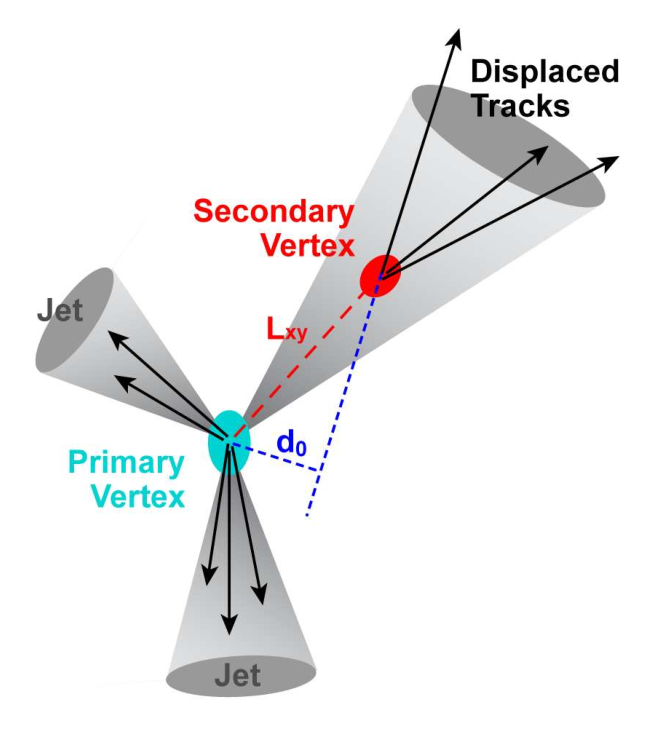
\includegraphics[width=0.8\textwidth]{evtsel/figs/secondaryVTX.pdf}
    \caption{
      \label{fig:secondaryVTX}
      A diagram showing a jet forming away from the primary vertex of a heavy flavor parton, for example a b or c quark.
    }
  \end{center}
\end{figure}

\begin{figure}[!ht]
  \begin{center}
      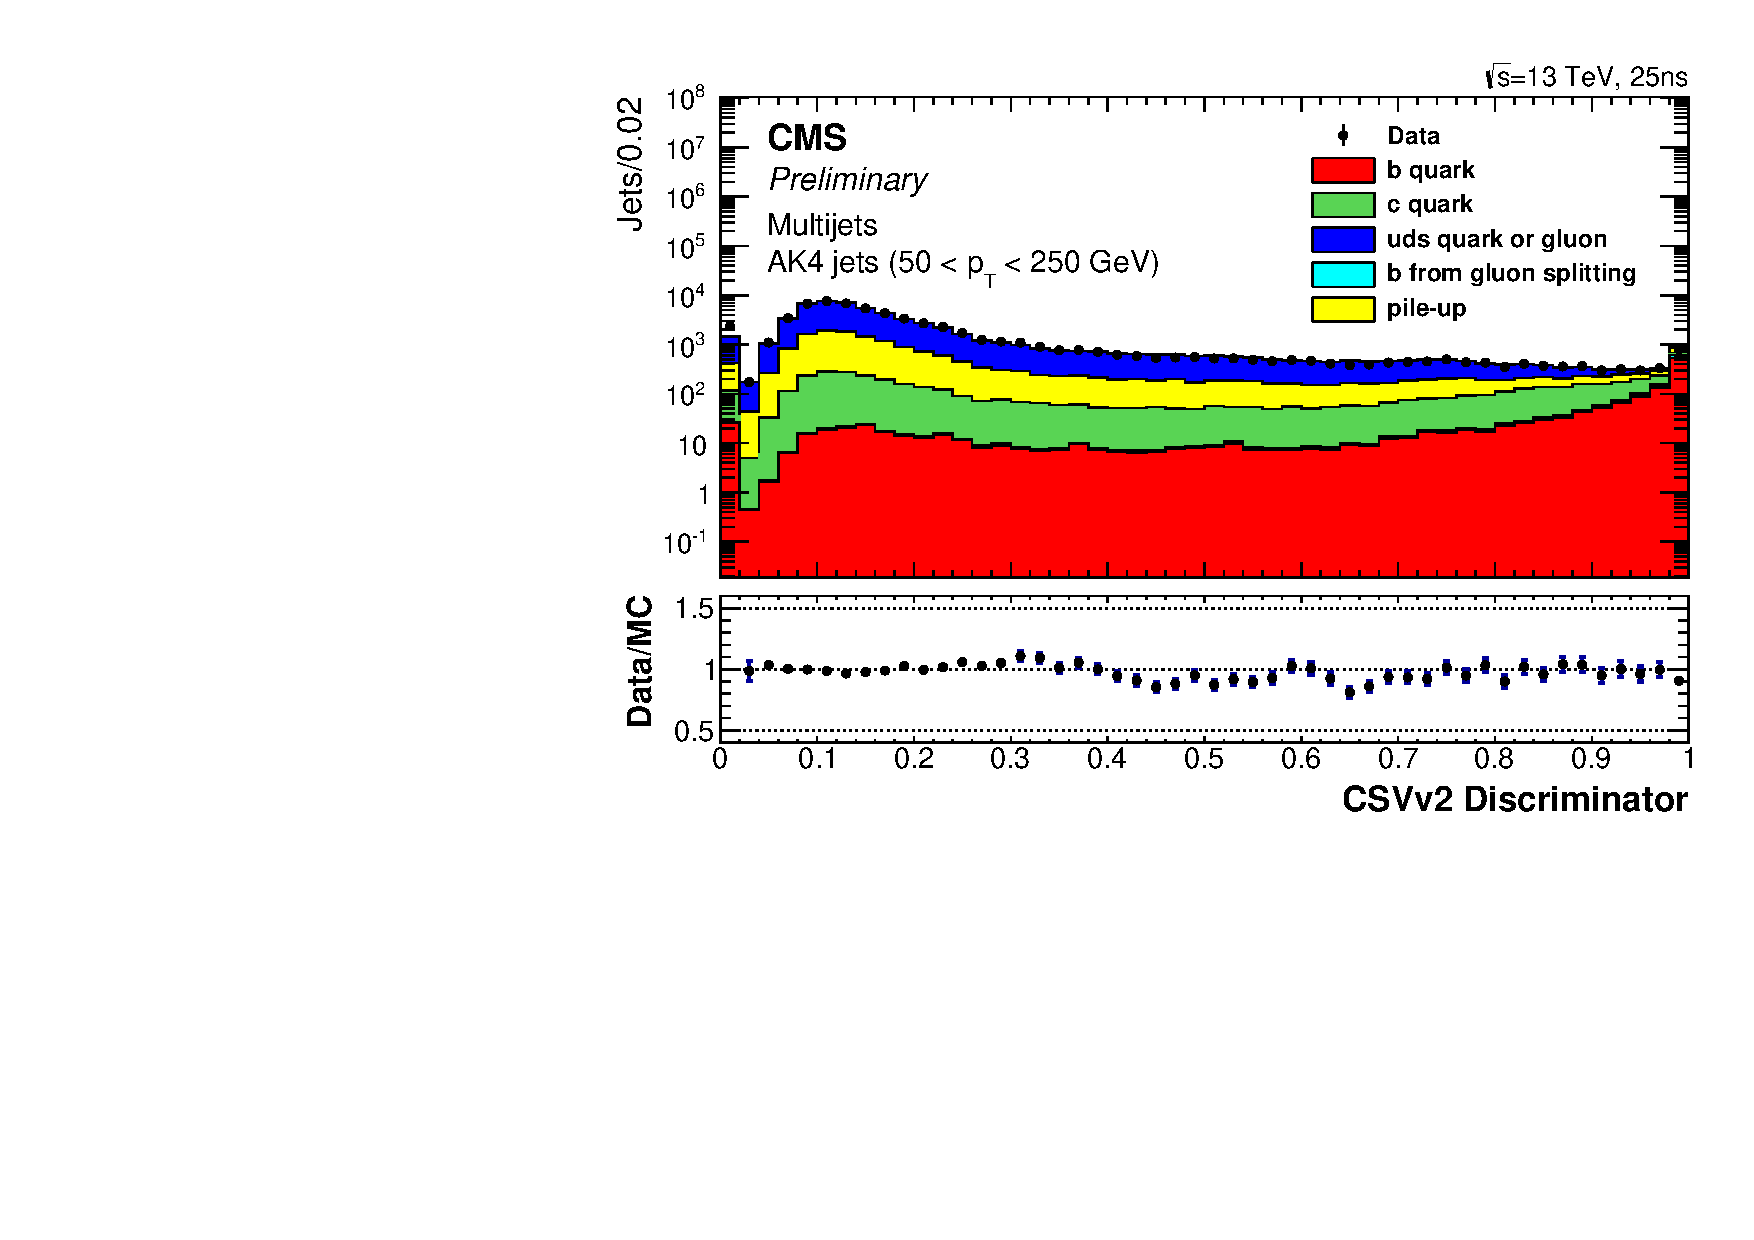
\includegraphics[width=0.8\textwidth]{evtsel/figs/ak4Inclusive_CSVIVF_Log.pdf}
    \caption{
      The distribution showing the CSVv2 Discriminator is shown comparing data vs. MC.
      The MC is split by jet parton flavor.
      \label{fig:csv}
    }
  \end{center}
\end{figure}

\subsection{Signal Region Definitions}
\label{sec:SRs}
Multiple, orthogonal signal regions are based on cuts on the number of jets, \Ht, and \MET.
These regions are then divided up into two categories, with and without b-tags.
The signal regions are classified into two separate categories called the ``A'' signal regions and ``B'' signal regions.
The ``A'' regions are defined as having \Ht\ $>~400$~\gev\ and 2-3 jets,
whereas the ``B'' regions are defined as having at least 4 jets. 
This leads to 16 orthogonal signal regions.
These regions are analyzed separately and then eventually combined to interpret results using the signal model described in~\ref{sec:signalmodel}.

In addition to the inclusive signal regions listed, a special signal region is defined which is designed to probe the region where a 3.0~$\sigma$~excess was seen in run-I by ATLAS~\cite{ATLASZPAPER}.
The requirements of this signal region in this analysis are as follows:

\begin{itemize}
\item at least 2 jets
\item $\mathrm{H_{T}+p_{T}(\ell_1)+p_{T}(\ell_2) > }$600 \gev
\item \MET~$>$~225 \gev
\item $\Delta\phi($\MET$,jet_{1,2})>$~0.4
\end{itemize}

\subsection{Selection Summary}
\label{sec:selsummary}
This section summarizes all of the object selections used in this analysis.
The preselection and the signal region selections are summarized in table~\ref{tab:selections}.

%% selections table
\begin{table}[htb]
\begin{center}
\caption{\label{tab:selections} List of all selections used to define the preselection and signal regions. }
\begin{tabular}{l|l}
\hline
\hline
preselection & \\
\hline
2 OSSF leptons (ee, $\mu\mu$)       & \pt\ $>$ 20 \gev, $|\eta| < 2.4$ \\
Dilepton invariant mass             &  81$<$\mll$<$101 \gev            \\
Jets                                & \pt\ $>$ 35 \gev, $|\eta| < 2.4$ \\
Minimum number of jets              & $\geq$2                          \\
b-tag requirement (medium)          & CSVv2IVF $>$ 0.890               \\
\hline                                          
\hline                                          
Signal selections         & \\
\hline                                          
b-tag requirements        & \\
\hline                                         
$\mathrm{N_{b-tags}}$ & $=$~0    \\
$\mathrm{N_{b-tags}}$ & $\geq$~1 \\
\hline                                          
\MET\ binning & \\
\hline                                          
\MET    & 100 - 150 \gev \\
\MET    & 150 - 225 \gev \\
\MET    & 225 - 300 \gev \\
\MET    & $>$ 300 \gev   \\
\hline                                          
A Signal regions    & $\mathrm{N_{jets}}~=$~2 or 3 and \Ht$\geq$~400 GeV \\
B Signal regions    & $\mathrm{N_{jets}} \geq$~4                         \\
ATLAS Signal region & $\mathrm{N_{jets}} \geq$~2, $\mathrm{H_{T}+p_{T}(\ell_1)+p_{T}(\ell_2) > }$600 \gev, \\
                    & $\Delta\phi($\MET$,jet_{1,2})>$~0.4, \MET~$>$~225 \gev \\
\hline                                          
\hline
\end{tabular}
\end{center}
\end{table}
